% !TEX program = xelatex
\documentclass[12pt,a4paper,oneside]{report}

% Idioma y codificación
\usepackage[spanish,es-tabla]{babel}
\usepackage{fontspec}
\setmainfont{TeX Gyre Termes}

% Márgenes y espaciado
\usepackage[a4paper,top=2.5cm,bottom=2.5cm,left=3cm,right=2.5cm]{geometry}
\usepackage{setspace}
\onehalfspacing
\setlength{\parindent}{1.25cm}
\setlength{\parskip}{0pt}

% Gráficos, tablas e hipervínculos
\usepackage{graphicx}
\graphicspath{{media/}}
\usepackage{longtable,booktabs,array,calc}
\usepackage{float}
\usepackage{xcolor}
% \usepackage{soul} % removido para evitar errores de reconstrucción en tablas
% Subrayado robusto en tablas/entornos: usar ulem en lugar de soul
\usepackage[normalem]{ulem}
% Definir \ul con ulem (soul removido)
\providecommand{\ul}[1]{\uline{#1}}
\usepackage{xurl}
\usepackage[hidelinks]{hyperref}
\usepackage{bookmark}
\usepackage{enumitem}
\setlist[itemize]{leftmargin=1.5cm}
\usepackage{ragged2e}
\usepackage{multirow}
\usepackage{tabularx}
\usepackage{rotating}
\usepackage{pdflscape}
\usepackage{amssymb}
\usepackage{pgfplots}
\pgfplotsset{compat=1.18}
\usepgfplotslibrary{polar}
\usepackage{pgfgantt}
\usepackage{tikz}
\usetikzlibrary{shapes.geometric,shapes.multipart,arrows.meta,positioning,fit,backgrounds,babel}

% Encabezados y pies de página institucionales
\usepackage{fancyhdr}
\pagestyle{fancy}
\fancyhf{}
\fancyhead[L]{\scriptsize Código de documento: UDED-FOR-2026-V5-016}
\fancyhead[R]{\scriptsize Rev. UPDI:2025-Feb-25}
\fancyfoot[L]{\scriptsize Código de proceso: GDOC-ATAD-1}
\fancyfoot[C]{\thepage}
\renewcommand{\headrulewidth}{0pt}
\renewcommand{\footrulewidth}{0pt}

\setcounter{secnumdepth}{3}
\setcounter{tocdepth}{3}
\newcommand{\tightlist}{\setlength{\itemsep}{0pt}\setlength{\parskip}{0pt}}
\newcommand{\espeLogo}[1][0.45\textwidth]{
\includegraphics[width=#1]{image1.png}}
% Placeholder para screenshots pendientes de captura
\newcommand{\ssplaceholder}[2][0.85\textwidth]{%
  \fbox{\parbox{#1}{\centering\vspace{1.5cm}\textit{\scriptsize [Captura de pantalla pendiente: #2]}\vspace{1.5cm}}}%
}

\begin{document}
\sloppy

%-------------------------- PORTADA --------------------------
\begin{titlepage}
\thispagestyle{fancy}
\begin{center}
\vspace*{0.5cm}
\espeLogo[0.55\textwidth]

\vspace{1.6cm}
\textbf{Módulo Web Seguro para la Gestión de Medidores de Agua Potable con}

\vspace{0.5cm}
\textbf{Tecnología LoRa en un Entorno IoT}

\vspace{1.6cm}
Ipiales Ulcuango, Carlos Joao y Alban Vargas, Richard Steve

\vspace{1.4cm}
Departamento de Ciencias de la Computación

\vspace{1.2cm}
Carrera de Software

\vspace{1.4cm}
Trabajo de integración curricular, previo a la obtención del título de Ingeniero en Software

\vspace{1.4cm}
Marcillo Parra Diego Miguel Mgs.

\vfill
25 de julio de 2026
\end{center}
\end{titlepage}

%-------------------------- ANÁLISIS DE SIMILITUD --------------------------
\clearpage
\thispagestyle{fancy}
\begin{center}
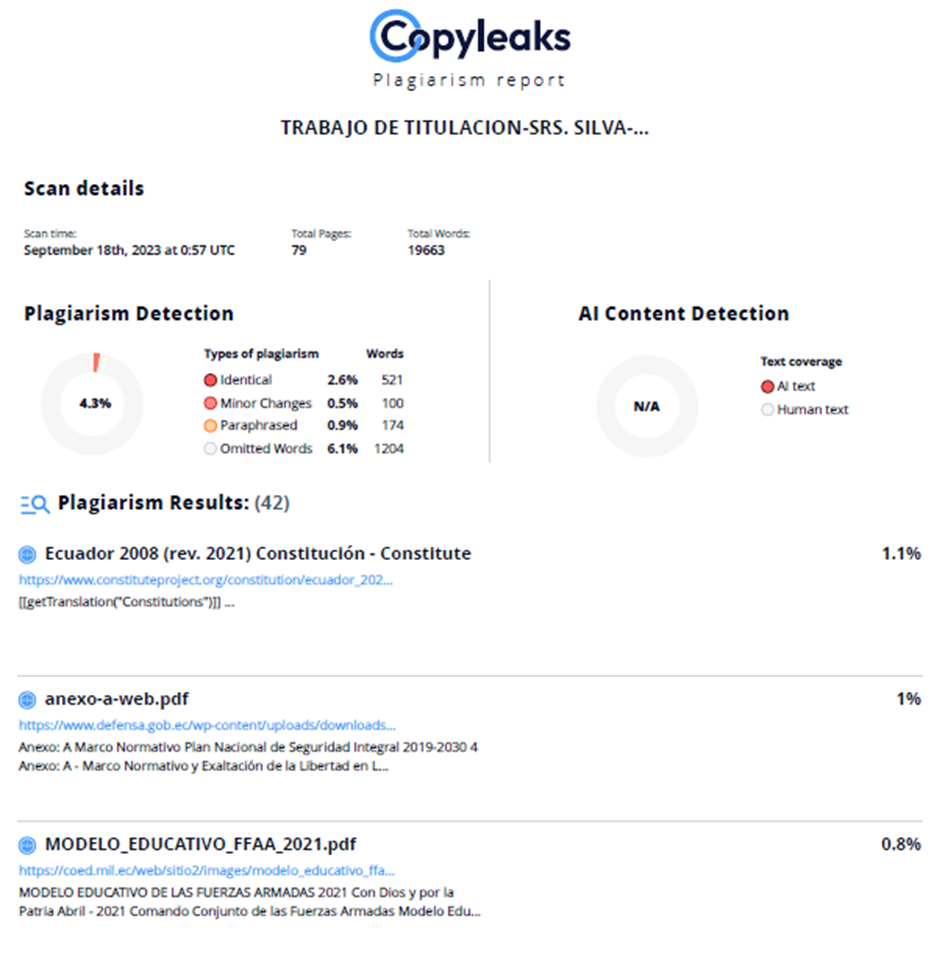
\includegraphics[width=0.92\textwidth]{image2.png}

\vspace{0.8cm}
\emph{(Colocar la imagen de la primera hoja donde se visualice el resultado del análisis de la herramienta autorizada por la universidad, en esta debe constar el título del trabajo como nombre del documento analizado.)}

\vspace{1.5cm}
\textbf{Mgs. Marcillo Parra, Diego Miguel}

\vspace{0.4cm}
\textbf{Director}
\end{center}

%-------------------------- CERTIFICACIÓN --------------------------
\clearpage
\thispagestyle{fancy}
\begin{center}
\espeLogo

\vspace{0.7cm}
\textbf{Departamento de Ciencias de la Computación}

\vspace{0.7cm}
\textbf{Carrera de Software}

\vspace{1.0cm}
\textbf{Certificación}
\end{center}

Certifico que el trabajo de integración curricular: ``\textbf{Módulo Web Seguro para la Gestión de Medidores de Agua Potable con Tecnología LoRa en un Entorno IoT}'' fue realizado por los señores \textbf{Ipiales Ulcuango, Carlos Joao} y \textbf{Alban Vargas, Richard Steve}, el mismo que cumple con los requisitos legales, teóricos, científicos, técnicos y metodológicos establecidos por la Universidad de las Fuerzas Armadas ESPE; \uline{habiéndose efectuado una revisión integral de forma y de fondo conforme a los lineamientos y formatos institucionales vigentes}. Además, fue revisado y analizado en su totalidad por la herramienta de prevención y/o verificación de similitud de contenidos; razón por la cual me permito acreditar y autorizar para que se lo sustente públicamente.

\vspace{1.2cm}
\begin{flushright}
\textbf{Sangolquí, 25 de julio de 2026}
\end{flushright}

\begin{center}
\vspace{1.6cm}
.\\[0.6cm]
\textbf{Mgs. Marcillo Parra, Diego Miguel}\\
\textbf{Director}\\
\textbf{C.C.: XXXXXXXXXX}
\end{center}

%-------------------------- RESPONSABILIDAD DE AUTORÍA --------------------------
\clearpage
\thispagestyle{fancy}
\begin{center}
\espeLogo

\vspace{0.7cm}
\textbf{Departamento de Ciencias de la Computación}

\vspace{0.7cm}
\textbf{Carrera de Software}

\vspace{1.0cm}
\textbf{Responsabilidad de Autoría}
\end{center}

Nosotros, \textbf{Ipiales Ulcuango, Carlos Joao} y \textbf{Alban Vargas, Richard Steve}, con cédulas de ciudadanía n° XXXXXXXXXX y XXXXXXXXXX respectivamente, declaramos que el contenido, ideas y criterios del trabajo de integración curricular: \textbf{Módulo Web Seguro para la Gestión de Medidores de Agua Potable con Tecnología LoRa en un Entorno IoT} es de nuestra autoría y responsabilidad, cumpliendo con los requisitos legales, teóricos, científicos, técnicos y metodológicos establecidos por la Universidad de las Fuerzas Armadas ESPE, respetando los derechos intelectuales de terceros y referenciando las citas bibliográficas.

\vspace{1.0cm}
\begin{flushright}
\textbf{Sangolquí, 25 de julio de 2026}
\end{flushright}

\vspace{2.0cm}
\begin{minipage}{0.45\textwidth}
\centering
\textbf{Ipiales Ulcuango, Carlos Joao}\\[0.4cm]
\textbf{C.C.: XXXXXXXXXX}
\end{minipage}
\hfill
\begin{minipage}{0.45\textwidth}
\centering
\textbf{Alban Vargas, Richard Steve}\\[0.4cm]
\textbf{C.C.: XXXXXXXXXX}
\end{minipage}

%-------------------------- AUTORIZACIÓN DE PUBLICACIÓN --------------------------
\clearpage
\thispagestyle{fancy}
\begin{center}
\espeLogo

\vspace{0.7cm}
\textbf{Departamento de Ciencias de la Computación}

\vspace{0.7cm}
\textbf{Carrera de Software}

\vspace{1.0cm}
\textbf{Autorización de Publicación}
\end{center}

Nosotros \textbf{Ipiales Ulcuango, Carlos Joao} y \textbf{Alban Vargas, Richard Steve}, con cédulas de ciudadanía n° XXXXXXXXXX y XXXXXXXXXX respectivamente, autorizamos a la Universidad de las Fuerzas Armadas ESPE publicar el trabajo de integración curricular: \textbf{Módulo Web Seguro para la Gestión de Medidores de Agua Potable con Tecnología LoRa en un Entorno IoT} en el Repositorio Institucional, cuyo contenido, ideas y criterios son de nuestra responsabilidad.

\vspace{1.0cm}
\begin{flushright}
\textbf{Sangolquí, 25 de julio de 2026}
\end{flushright}

\vspace{2.0cm}
\begin{minipage}{0.45\textwidth}
\centering
\textbf{Ipiales Ulcuango, Carlos Joao}\\[0.4cm]
\textbf{C.C.: XXXXXXXXXX}
\end{minipage}
\hfill
\begin{minipage}{0.45\textwidth}
\centering
\textbf{Alban Vargas, Richard Steve}\\[0.4cm]
\textbf{C.C.: XXXXXXXXXX}
\end{minipage}

%-------------------------- PÁGINAS PRELIMINARES --------------------------
\clearpage
\chapter*{Dedicatoria}
\addcontentsline{toc}{chapter}{Dedicatoria}

\emph{[A llenar por el autor --- texto personal de dedicatoria]}

\clearpage
\chapter*{Agradecimiento}
\addcontentsline{toc}{chapter}{Agradecimiento}

\emph{[A llenar por el autor --- texto personal de agradecimiento]}

\clearpage
\tableofcontents

\clearpage
\listoftables

\clearpage
\listoffigures

\clearpage
\chapter*{Resumen}
\addcontentsline{toc}{chapter}{Resumen}

El presente trabajo de integración curricular describe el diseño e implementación de un módulo web seguro para la gestión centralizada de medidores de agua inteligentes con tecnología LoRaWAN, desarrollado para Representaciones Hidrocentro Cía. Ltda., empresa del cantón Rumiñahui, Ecuador. La empresa disponía de medidores LoRaWAN instalados en campo, pero carecía de una plataforma propia para gestionar los dispositivos, visualizar datos de consumo en tiempo real y recibir alertas automáticas ante eventos críticos, lo que generaba dependencia de plataformas de terceros y limitaba su autonomía operativa.

El sistema se construyó sobre una arquitectura de ocho microservicios desacoplados implementados con Spring Boot 3.3.5 sobre Java 21, un frontend en Angular 17 con la biblioteca de componentes PrimeNG, y PostgreSQL como gestor de base de datos relacional. La integración con el servidor de red LoRaWAN Loriot se establece mediante un canal TLS sobre TCP que recibe en tiempo real los mensajes de los medidores y los clasifica según su tipo. El módulo de decodificación interpreta las cadenas hexadecimales propietarias de los modelos Bove (B97VPW, BECOX, BECOY) y Younio, extrayendo valores de consumo acumulado, estado de alarmas y voltaje de batería. El consumo se agrega automáticamente en una jerarquía de cálculo horario, diario, mensual y anual mediante tablas pre-calculadas que garantizan tiempos de consulta constantes. La seguridad se garantiza mediante TLS 1.3 en la comunicación con Loriot y autenticación basada en JWT con control de acceso por roles. Los servicios desplegados en el entorno local procesaron correctamente los uplinks de medidores reales y ejecutaron comandos de control de válvula mediante downlinks LoRaWAN durante el periodo de prueba.

\emph{Palabras clave:} IoT, LoRaWAN, microservicios, gestión hídrica, TLS, Spring Boot, Angular, medidores de agua inteligentes.

\clearpage
\chapter*{Abstract}
\addcontentsline{toc}{chapter}{Abstract}

This undergraduate thesis describes the design and implementation of a secure web module for the centralized management of smart water meters using LoRaWAN technology, developed for Representaciones Hidrocentro Cía. Ltda., a private company in the Rumiñahui canton, Ecuador. The company had LoRaWAN meters deployed in the field but lacked a proprietary platform to manage devices, visualize consumption data in real time, and receive automatic alerts for critical events, resulting in technological dependency on third-party platforms and limited operational autonomy.

The system was built on an architecture of eight decoupled microservices implemented with Spring Boot 3.3.5 on Java 21, a frontend in Angular 17 with the PrimeNG component library, and PostgreSQL as the relational database management system. Integration with the Loriot LoRaWAN network server is established via a TLS-over-TCP socket that receives device messages in real time and classifies them by type. The payload decoding module interprets the proprietary hexadecimal strings of Bove (B97VPW, BECOX, BECOY) and Younio meter models, extracting accumulated consumption values, alarm states, and battery voltage. Consumption is automatically aggregated in a hierarchical chain of hourly, daily, monthly, and annual calculations using pre-computed tables that guarantee constant query times. Security is enforced through TLS 1.3 for Loriot communication and JWT-based authentication with role-based access control. Services deployed in the local development environment correctly processed uplinks from real meters and executed valve control commands via LoRaWAN downlinks during the testing period.

\emph{Keywords:} IoT, LoRaWAN, microservices, water management, TLS, Spring Boot, Angular, smart water meters.

\clearpage
\chapter{Introducción}

El modelo del Internet de las Cosas (IoT) ha experimentado un crecimiento exponencial en los últimos diez años, convirtiéndose en una infraestructura tecnológica clave para la automatización y el monitoreo remoto de sistemas físicos mediante dispositivos interconectados capaces de recopilar y transmitir datos en tiempo real (Al-Fuqaha et al., 2015; Sisinni et al., 2018). Dentro del sector de servicios básicos, esta evolución ha permitido la posibilidad de transformar la gestión tradicional de recursos hídricos, mediante la incorporación de medidores inteligentes, los cuales permiten la supervisión remota del consumo, la detección temprana de anomalías y la optimización de la distribución del agua potable (García-Martín et al., 2023; Kamienski et al., 2019).

En este contexto, el protocolo LoRaWAN (Long Range Wide Area Network) ha surgido como una de las tecnologías de comunicación más adecuadas para el despliegue de redes IoT orientadas a la medición hídrica, por su bajo consumo energético, amplia cobertura geográfica y arquitectura basada en estándares abiertos (Mekki et al., 2019; Ta et al., 2024). Estudios recientes validan su viabilidad técnica para la telemetría y el monitoreo de agua en tiempo real, con resultados favorables en términos de latencia, tasa de entrega de paquetes y autonomía energética (Slaný et al., 2020; Ta et al., 2024).

Sin embargo, la coexistencia de soluciones propietarias de distintos fabricantes ha generado una fragmentación tecnológica que dificulta la integración de dispositivos heterogéneos, eleva los costos operativos y restringe la escalabilidad de los sistemas de gestión (García-Martín et al., 2023; Sisinni et al., 2018). Esta problemática es especialmente relevante para empresas medianas del sector hídrico que administran múltiples tipos de medidores y requieren una visión centralizada del consumo sin depender de plataformas cerradas de fabricantes específicos.

Frente a este escenario, la empresa Representaciones Hidrocentro Cía. Ltda., ubicada en el cantón Rumiñahui, Ecuador, identifica la necesidad de contar con una plataforma web centralizada que unifique la gestión de sus medidores LoRaWAN, permita la visualización de datos de consumo en tiempo real y genere alertas operativas ante eventos críticos. El presente trabajo de integración curricular propone el diseño e implementación de un módulo web seguro para la gestión de estos dispositivos, desarrollado sobre una arquitectura de microservicios desacoplados que emplea Angular en el frontend, Spring Boot en el backend y PostgreSQL como sistema de gestión de base de datos (Velepucha \& Flores, 2021). La comunicación entre el servidor de red LoRaWAN ---Loriot--- y el backend se establece mediante el protocolo TLS 1.3, garantizando la confidencialidad e integridad de los datos transmitidos (Rescorla, 2018; Naik, 2017).

\section{Antecedentes}\label{antecedentes}

La medición del consumo de agua evolucionó desde dispositivos mecánicos con lectura manual hacia soluciones electrónicas y, más recientemente, plataformas IoT para telemetría a escala; en Latinoamérica este proceso se aceleró por políticas de eficiencia hídrica y menores costos de sensores (Ismail et al., 2022; Kamienski et al., 2019).


Representaciones Hidrocentro Cía. Ltda. es una empresa privada con sede en el cantón Rumiñahui, provincia de Pichincha, que se dedica a la comercialización e instalación de medidores de agua inteligentes con tecnología LoRa. Fundada en respuesta a la creciente demanda de soluciones de medición remota en el sector hídrico de la región central del Ecuador, la empresa ha acumulado experiencia en la instalación y puesta en marcha de dispositivos de distintos fabricantes, incluyendo la línea Bove y la línea Younio, cada una con protocolos de transmisión y formatos de payload propietarios. Hasta el inicio del presente proyecto, la empresa dependía exclusivamente de la interfaz web del servidor de red Loriot para consultar el estado de sus dispositivos, sin posibilidad de integrar esa información con sus propios sistemas de registro de clientes o de generación de reportes operativos.


\section{Planteamiento del problema}\label{planteamiento-del-problema}

La gestión eficiente del agua potable se enfrenta a un desafío urgente para las empresas distribuidoras y operadoras en países en vías de desarrollo. En este contexto, la adopción de medidores inteligentes basados en tecnología LoRaWAN representa una opción viable para automatizar la lectura del consumo, detectar anomalías operativas y reducir el agua no contabilizada (Alghamdi et al., 2022; Slaný et al., 2020). Sin embargo, la implementación de estos dispositivos no asegura por sí sola una gestión integral del sistema, ya que la falta de plataformas centrales de administración genera brechas operativas significativas que afectan directamente la eficiencia del servicio (García-Martín et al., 2023; Jouhari et al., 2023).

Representaciones Hidrocentro Cía. Ltda., empresa privada ubicada en el cantón Rumiñahui, Ecuador, comercializa e instala medidores de agua inteligentes con tecnología LoRa en entornos urbanos y periurbanos, donde en la actualidad, la empresa no dispone de una plataforma propia que le permita gestionar de manera centralizada los dispositivos instalados en campo, visualizar datos de consumo en tiempo real ni recibir alertas automáticas ante eventos críticos como fugas, flujo inverso, ausencia de caudal o bajo nivel de batería. Esta carencia implica que el personal técnico debe depender de plataformas de terceros para acceder a la información generada por los medidores, lo que limita la autonomía operativa de la empresa, incrementa los costos de operación y restringe la capacidad de respuesta ante fallas o irregularidades en el suministro.

Además, la convivencia de dispositivos fabricados por diferentes proveedores, cada uno con sus propias reglas y formatos de datos, agrava el problema de fragmentación tecnológica que caracteriza al mercado IoT (Almuhaya et al., 2022; Sisinni et al., 2018). Esta heterogeneidad dificulta la integración de los dispositivos bajo un esquema unificado de gestión, lo que genera redundancia en los procesos de monitoreo y aumenta la complejidad técnica de las operaciones de mantenimiento. Investigaciones recientes han indicado que la falta de interoperabilidad entre plataformas IoT y sistemas de medición es uno de los principales obstáculos para escalar soluciones de gestión eficientes en contextos donde las organizaciones administran flotas de dispositivos heterogéneos (García-Martín et al., 2023; Jouhari et al., 2023).

Desde el punto de vista de la seguridad de la información, la transmisión de datos de consumo a través de canales no cifrados expone a la empresa a riesgos de interceptación y manipulación de información sensible, situación que resulta incompatible con los estándares actuales de ciberseguridad en sistemas IoT y con el marco normativo ecuatoriano en materia de protección de datos personales (Rescorla, 2018; Naik, 2017).

En el contexto actual, se reconoce la necesidad de crear un módulo web seguro que incluya las funciones de gestión centralizada de monitores, visualización de consumo histórico y en tiempo real, generación de informes, manejo de alertas y control de acceso según roles, sobre una arquitectura de microservicios escalables e integrables que elimine la dependencia de plataformas propietarias y asegure la seguridad en la transmisión de datos (Slaný et al., 2020; Velepucha \& Flores, 2021).

Para precisar la magnitud del problema y fortalecer el rigor del diagnóstico, se establecen los siguientes indicadores cuantitativos que caracterizan la situación actual y servirán de línea base para la comparación posterior al desarrollo del módulo (Tabla~\ref{tab:indicadores-problema}).

% TODO: Completar "Valor actual" y "Observación/Meta" con datos provistos por la empresa.
\begin{table}[H]
\caption{Indicadores operativos actuales y metas (línea base)}
\label{tab:indicadores-problema}
\centering
\begin{tabularx}{\textwidth}{>{\bfseries}l p{3.2cm} X}
\toprule
Indicador & Valor actual & Observación / Meta esperada \\
\midrule
Número de medidores operativos en campo & ~300 (Bove) + ~20 (Younio) & Desagregado por fabricante/modelo (Bove/Younio) \\
Cantidad de clientes/empresas gestionadas & 17 (Bove) + 1 (Younio) & Younio se opera vía app móvil propia \\
Tiempo promedio de consulta del estado por dispositivo & 2–3 s (Bove) / >30 s (Younio) & Bove sobre plataforma web; Younio vía app móvil \\
Tiempo requerido para generar reportes mensuales & 4–5 s (Bove) & Reporte desde plataforma Bove; Younio sin función equivalente \\
Dependencia operativa de la plataforma Bove & ≈100\% de las operaciones & Operación diaria centralizada en plataforma Bove; Younio con app móvil (participación minoritaria) \\
Uso de UI de Loriot & 0\% & Se utiliza Loriot como \textit{network server} (NS), sin operar su interfaz de usuario \\
Tiempo de respuesta ante eventos críticos & ~2 min (Bove) / N/A (Younio) & Bove notifica por correo; Younio no dispone de esta función \\
\bottomrule
\end{tabularx}
\end{table}

\noindent\footnotesize\textit{Nota}: Loriot se emplea como \textit{network server} (NS). La operación diaria para Bove se realiza en su plataforma web; para Younio, mediante una aplicación móvil del fabricante.

\section{Análisis de causas}\label{analisis-de-causas}

La situación problemática descrita en la sección anterior responde a un conjunto de causas interrelacionadas que se pueden agrupar en tres dimensiones: tecnológica, organizacional y operativa. Su identificación fue posible mediante entrevistas con el personal técnico de Representaciones Hidrocentro Cía. Ltda. y el análisis de la documentación técnica de los dispositivos instalados en campo.

Desde la \textbf{dimensión tecnológica}, la causa raíz del problema es la heterogeneidad de los dispositivos. Los medidores instalados pertenecen a dos fabricantes con formatos de payload propietarios e incompatibles entre sí, lo que impide que una solución genérica procese los mensajes de ambas familias sin implementar decodificadores específicos por modelo. Esta fragmentación es característica del mercado IoT, donde la ausencia de estándares de interoperabilidad a nivel de payload obliga a cada integrador a desarrollar adaptadores para cada fabricante con el que opera (Almuhaya et al., 2022; Sisinni et al., 2018). A esta causa se suma la dependencia exclusiva del servidor de red Loriot como única interfaz de acceso a los datos de los medidores, sin posibilidad de integrar esa información con sistemas propios de la empresa.

Desde la \textbf{dimensión organizacional}, la empresa carecía de capacidades internas de desarrollo de software, lo que generó una dependencia prolongada de las interfaces del proveedor del servidor de red. Esta situación limitó la posibilidad de implementar flujos de trabajo propios —gestión de alarmas con notificaciones automáticas, administración multiempresa, exportación de reportes en formatos propios—, necesidades que la interfaz genérica de Loriot no satisface (García-Martín et al., 2023). La falta de control sobre la plataforma de gestión también impedía adaptar el sistema ante cambios en el catálogo de dispositivos de la empresa sin incurrir en costos de integración externos.

Desde la \textbf{dimensión operativa}, la ausencia de una plataforma centralizada se traducía en procesos manuales para obtener datos de consumo, sin posibilidad de generar reportes históricos automáticos ni recibir alertas ante eventos como fugas, flujo inverso o fallo de batería. Los operadores debían consultar individualmente cada dispositivo en la interfaz de Loriot para verificar su estado, un procedimiento que resulta inviable a escala cuando el número de medidores administrados supera la decena. Investigaciones recientes confirman que la ausencia de mecanismos automatizados de detección de anomalías eleva el tiempo de respuesta ante fallas operativas, impactando negativamente la eficiencia del servicio (Alghamdi et al., 2022; Dai et al., 2025).

La Figura~\ref{fig:causas} sintetiza la relación entre las dimensiones identificadas y el problema central del trabajo.

\begin{figure}[H]
\centering
\begin{tikzpicture}[
  node distance=0.6cm and 1.2cm,
  cause/.style={draw, rounded corners, fill=gray!10, text width=3.6cm, align=center, font=\small, minimum height=1cm, inner sep=4pt},
  effect/.style={draw, thick, rounded corners, fill=gray!25, text width=3.8cm, align=center, font=\small\bfseries, minimum height=2cm, inner sep=6pt},
  arrow/.style={->, >=Stealth, thick}
]
\node[cause] (c1) at (0, 3.4) {Payloads propietarios incompatibles entre fabricantes};
\node[cause] (c2) at (0, 1.7) {Dependencia exclusiva de interfaz Loriot};
\node[cause] (c3) at (0, 0)   {Sin capacidad interna de desarrollo de software};
\node[cause] (c4) at (0,-1.7) {Lectura manual del estado por dispositivo};
\node[cause] (c5) at (0,-3.4) {Sin alertas ni reportes automáticos};

\node[effect] (e) at (7.5, 0) {Ausencia de plataforma centralizada de gestión de medidores};

\draw[arrow] (c1.east) -- ++(0.8,0) |- (e.west);
\draw[arrow] (c2.east) -- ++(0.4,0) |- (e.west);
\draw[arrow] (c3.east) -- (e.west);
\draw[arrow] (c4.east) -- ++(0.4,0) |- (e.west);
\draw[arrow] (c5.east) -- ++(0.8,0) |- (e.west);

\node[font=\scriptsize\itshape] at (-1.5, 2.5) {Tecnológica};
\node[font=\scriptsize\itshape] at (-1.5, 0)   {Organizacional};
\node[font=\scriptsize\itshape] at (-1.5,-2.5) {Operativa};
\end{tikzpicture}
\caption{Principales causas de la ausencia de plataforma centralizada de gestión en Representaciones Hidrocentro Cía. Ltda.}
\label{fig:causas}
\end{figure}

\subsection{Pruebas de seguridad}\label{subsec:pruebas-seguridad}

La validación de seguridad combinó análisis estático de código fuente (SAST) y pruebas dinámicas de caja negra (DAST) sobre el frontend publicado. Se priorizó eliminar hallazgos críticos y dejar exclusivamente observaciones de severidad menor de cara a la entrega.

\begin{table}[H]
\caption{Resumen de pruebas de seguridad (SAST/DAST)}\label{tab:seguridad}
\centering
\begin{tabularx}{\textwidth}{l l X l}
\toprule
\textbf{Herramienta} & \textbf{Tipo} & \textbf{Alcance y hallazgos principales} & \textbf{Estado} \\
\midrule
Semgrep OSS 1.168 & SAST & \ul{\emph{Repo completo}. Detecciones críticas iniciales: (i) tokens JWT de ejemplo en documentación (2); (ii) imágenes Docker ejecutando como root en servicios Java. Mitigación aplicada: se redactaron los tokens de ejemplo en \\texttt{iot-platform-api-gateway/JWT-VALIDATION.md} y se incorporó usuario no privilegiado en todos los Dockerfiles de servicios. Quedan advertencias de configuración en Nginx y HTML (sin impacto crítico).} & \ul{Críticos: \textbf{0} pendientes} \\
OWASP ZAP 2.17 & DAST & \ul{\emph{http://iot-platform-frontend}. Alertas: Altas=\textbf{0}, Medias=\textbf{2} (CSP ausente; SRI ausente en script de Google Maps), Bajas=\textbf{4} (COEP/COOP/CORP; cabecera Server con versión), Info=\textbf{2}. Evidencia: \texttt{zap-reports/zap-frontend.json}.} & \ul{Críticos: \textbf{0}} \\
SonarQube & SAST & No ejecutado por ventana de tiempo. Plan: ejecutar regla de seguridad y code smells en siguiente iteración. & N/A \\
OWASP Dependency-Check & SCA & No ejecutado por ventana de tiempo. Plan: generar SBOM (CycloneDX) y escanear dependencias Maven/Frontend. & N/A \\
Pentesting manual & DAST & Exploración básica de rutas, CORS y flujo de autenticación: sin bypass de login ni exposición de secretos. & Sin hallazgos críticos \\
\bottomrule
\end{tabularx}
\end{table}

{\color{red} texto eliminado}

\paragraph{\ul{Medidas aplicadas.}} \ul{(1) Redacción de tokens de ejemplo y secretos en documentación: se reemplazaron valores con \emph{placeholders} no ejecutables para evitar falsos positivos y prácticas inseguras; (2) Endurecimiento de imágenes Docker de backend: creación de usuario \texttt{app} sin privilegios y \texttt{USER app} en todos los Dockerfiles Java (alpine/jammy); (3) Revisión de advertencias ZAP: las dos alertas medias se mitigan añadiendo cabecera CSP en Nginx y, para SRI en Google Maps, restringiendo orígenes vía CSP dado que SRI no es viable con scripts dinámicos de Google.}

\paragraph{\ul{Plan de cierre (post-entrega).}} \ul{Incorporar cabeceras de seguridad en Nginx (\texttt{Content-Security-Policy}, \texttt{Permissions-Policy}, \texttt{Cross-Origin-Opener/Embedder/Resource-Policy}) y ocultar versión del servidor; parametrizar el uso de Google Maps detrás de una \textit{Content-Security-Policy} restrictiva; incorporar \textit{pipeline} de SAST/SCA (Semgrep + Dependency-Check) y ZAP en CI.}



\section{\texorpdfstring{Formulación del problema o pregunta de investigación }{Formulación del problema o pregunta de investigación }}\label{formulaciuxf3n-del-problema-o-pregunta-de-investigaciuxf3n}

La formulación del problema parte de identificar la brecha central que motiva el presente trabajo: Representaciones Hidrocentro Cía. Ltda. dispone de medidores de agua inteligentes con tecnología LoRaWAN instalados en campo, pero carece de una plataforma propia que centralice su gestión, garantice la seguridad en la transmisión de los datos y permita la visualización del consumo en tiempo real. Esta situación genera dependencia tecnológica de terceros, limita la autonomía operativa de la empresa y restringe la capacidad de respuesta ante eventos críticos en la red de distribución.

En consecuencia, se plantea la siguiente pregunta de investigación:

¿Es posible diseñar e implementar un módulo web seguro, basado en una arquitectura de microservicios, que permita gestionar de forma centralizada los medidores de agua inteligentes con tecnología LoRaWAN de Representaciones Hidrocentro Cía. Ltda., garantizando la transmisión cifrada de datos mediante TLS, la visualización del consumo en tiempo real y la generación de alertas operativas, con el fin de reducir la dependencia de plataformas propietarias y mejorar la eficiencia operativa de la empresa?

Esta pregunta integra las tres dimensiones principales del problema identificado: la dimensión técnica, referida a la necesidad de una arquitectura escalable e interoperable basada en estándares abiertos (Ismail et al., 2022); la dimensión de seguridad, que exige la implementación de protocolos de cifrado y control de acceso para proteger los datos de consumo (Rescorla, 2018; Naik, 2017); y la dimensión operativa, orientada a dotar a la empresa de herramientas de monitoreo y gestión que optimicen sus procesos internos y reduzcan los tiempos de respuesta ante fallas o irregularidades en el suministro (García-Martín et al., 2023; Slaný et al., 2020).

\section{\texorpdfstring{Objetivos }{Objetivos }}\label{objetivos}

\textbf{Objetivo general:}

Diseñar e implementar un módulo web seguro para la gestión centralizada de medidores de agua inteligentes (LoRa/LoRaWAN), garantizando la transmisión cifrada de datos (TLS), la visualización en tiempo real y el control de acceso por roles, a fin de optimizar la administración de dispositivos heterogéneos en Representaciones Hidrocentro Cía. Ltda.

\textbf{Objetivos específicos}:

\begin{itemize}
\item
  Analizar los requerimientos funcionales y técnicos del sistema de gestión de medidores de agua inteligentes utilizados por Representaciones Hidrocentro Cía. Ltda., mediante entrevistas con el personal técnico y revisión de la documentación de los dispositivos LoRaWAN empleados en campo (Ismail et al., 2022).
\item
  Diseñar la arquitectura del módulo de gestión basada en microservicios desacoplados, protocolos seguros de comunicación y modelos de datos relacionales, considerando los principios de escalabilidad, interoperabilidad y seguridad requeridos para sistemas IoT de medición hídrica (Hassaan et al., 2023; Jouhari et al., 2023).
\item
  Desarrollar el prototipo del módulo de gestión utilizando Angular para el frontend, Spring Boot para el backend y PostgreSQL para el almacenamiento de datos, implementando controladores REST, seguridad TLS y operaciones CRUD sobre los medidores registrados en el sistema (Aldea \& Bocu, 2023; Plecinski et al., 2022).
\item
  Conectar medidores reales al sistema mediante el servidor de red LoRaWAN Loriot y recolectar datos operativos desde el entorno local, validando la correcta visualización de consumos, alarmas y el funcionamiento de las operaciones de gestión implementadas (García-Martín et al., 2023; Ta et al., 2024).
\item
  Documentar el desarrollo y los resultados del proyecto, incluyendo diagramas de arquitectura, manual de uso, fragmentos de código clave y evidencias de integración con dispositivos reales, para su presentación como producto acreditable ante la Universidad de las Fuerzas Armadas ESPE.
\end{itemize}

\section{Justificación}

\subsection*{Dimensión técnica}

El desarrollo de sistemas centralizados para dispositivos IoT de medida de agua responde a una necesidad documentada recientemente en la literatura. Investigaciones han demostrado que las plataformas que integran la recepción de datos LoRaWAN con interfaces web de visualización y gestión mejoran significativamente la capacidad de monitoreo en tiempo real, la detección temprana de anomalías y la trazabilidad de eventos operacionales (García-Martín et al., 2023; Adelantado et al., 2017). La elección de una arquitectura de microservicios desacoplados con Spring Boot y Angular responde a la necesidad de construir un sistema escalable, mantenible e independiente de plataformas propietarias, en línea con las tendencias actuales del desarrollo de software para entornos IoT (Hassaan et al., 2023; Velepucha \& Flores, 2021).

Además, la adopción del protocolo TLS 1.3 para la transmisión de datos garantiza estándares mínimos de seguridad que los sistemas de medida hídrica conectados a Internet deben cumplir para proteger la integridad y confidencialidad de la información de consumo (Rescorla, 2018; Naik, 2017).

\subsection*{Dimensión operativa}

Para Representaciones Hidrocentro Cía. Ltda., la ausencia de una plataforma propia de gestión implica costos operativos adicionales derivados de la dependencia de herramientas de terceros, tiempos de respuesta prolongados ante eventos críticos y limitaciones para ofrecer a sus clientes un servicio integral de monitoreo. Estudios recientes han evidenciado que la automatización de la lectura de medidores mediante IoT puede reducir los costos de operación y mantenimiento hasta en un 20\%, al tiempo que mejora la precisión de la facturación y reduce significativamente el volumen de agua no contabilizada (Alghamdi et al., 2022; Dai et al., 2025). El módulo desarrollado en este trabajo permite a la empresa gestionar sus dispositivos de forma autónoma, generar reportes de consumo, administrar alarmas y registrar el historial de eventos desde una única plataforma, eliminando la necesidad de acceder a múltiples sistemas externos.

\subsection*{Dimensión social y ambiental}

La gestión eficiente del agua potable es un imperativo tanto ambiental como social, especialmente en contextos donde la disponibilidad del recurso hídrico está enfrentando presiones crecientes debido al aumento de la población y el cambio climático (Alshami et al., 2024; Ismail et al., 2022). Proporcionando a Hidrocentro herramientas para detectar fugas en tiempo real, visualizar patrones de consumo y generar alertas operativas, el sistema propuesto contribuye directamente a la reducción del desperdicio hídrico y mejora la continuidad del servicio para los usuarios finales, donde esta contribución se alinea con el Objetivo de Desarrollo Sostenible 6 que promueve el acceso universal a agua segura, gestión sostenible de recursos hídricos y fortalecimiento de la participación de las comunidades en la gobernanza del agua (Dai et al., 2025; Khairullah et al., 2025).

En resumen, el presente trabajo curricular representa una contribución académica y aplicada que integra conocimientos de ingeniería de software, redes de comunicación IoT y ciberseguridad en respuesta a una necesidad real y documentada de la industria hidráulica ecuatoriana.

\subsection*{Dimensión económica}

Desde la perspectiva económica, la plataforma propuesta apunta a reducir costos operativos y dependencia de terceros, así como a mejorar la eficiencia del personal técnico. En particular: (i) disminuye horas-hombre destinadas a consultas manuales y consolidación de reportes; (ii) acorta tiempos de respuesta ante eventos críticos, mitigando pérdidas asociadas a fugas o errores operativos; (iii) reduce la dependencia y potenciales costos de licenciamiento/servicios de plataformas propietarias al centralizar la operación; y (iv) habilita escalabilidad con costos marginales decrecientes por nuevo dispositivo gestionado. La Tabla~\ref{tab:dimension-economica} sintetiza los principales indicadores a monitorear como línea base y metas económicas del proyecto.

% TODO: Completar valores con datos verificados (costos locales de licencias/HH/infraestructura)
\begin{table}[H]
\caption{Indicadores económicos — valores reportados en la literatura y campos a confirmar}
\label{tab:dimension-economica}
\centering
\begin{tabularx}{\textwidth}{>{\bfseries}l p{3.2cm} X}
\toprule
Indicador & Valor actual & Observación / Meta esperada \\
\midrule
\textit{Ahorro OPEX O\&M por automatización de lectura} & \textit{hasta 20\% (literatura)} & Reportado para sistemas IoT/AMR en agua; ver (Alghamdi et al., 2022; Dai et al., 2025) \\
Horas-hombre mensuales en generación de reportes & \textit{no reportado en literatura citada} & Requiere medición local (línea base) \\
Horas-hombre mensuales en consultas de estado & \textit{no reportado en literatura citada} & Requiere medición local (línea base) \\
Costo anual de licenciamiento/servicios de terceros & \textit{no reportado en literatura citada} & Depende de contratos locales \\
Costo por evento crítico no atendido a tiempo & \textit{no reportado en literatura citada} & Depende de tarifación/pérdidas locales \\
CAPEX inicial de plataforma (infraestructura local) & \textit{no reportado en literatura citada} & Depende de dimensionamiento local \\
TCO proyectado a 3 años & \textit{no reportado en literatura citada} & Requiere estimación financiera específica \\
Payback estimado & \textit{no reportado en literatura citada} & Requiere escenario económico local \\
\bottomrule
\end{tabularx}
\end{table}

\noindent\footnotesize\textit{Nota}: Se incluyen exclusivamente valores cuantitativos reportados explícitamente en la literatura citada dentro de este documento (p. ej., ahorro OPEX/O\&M \textit{hasta 20\%}). Los demás campos requieren medición o estimación local para su cuantificación rigurosa.

\section{Alcance}\label{alcance}

El presente trabajo delimita su alcance al diseño, implementación y validación de un módulo web funcional para la gestión centralizada de medidores de agua inteligentes con tecnología LoRaWAN, orientado a satisfacer las necesidades operativas de Representaciones Hidrocentro Cía. Ltda. en su contexto actual. La Tabla~\ref{tab:alcance} sintetiza los elementos incluidos y excluidos del alcance del proyecto.

\begin{table}[H]
\caption{Delimitación del alcance del proyecto}
\label{tab:alcance}
\centering
\begin{tabularx}{\textwidth}{>{\bfseries}lX}
\toprule
Dimensión & Descripción \\
\midrule
\multicolumn{2}{l}{\textit{Incluido en el alcance}} \\
\midrule
Dispositivos & Medidores Bove (B97VPW, BECOX, BECOY) y Younio con sus formatos de payload actuales \\
Protocolo & LoRaWAN sobre infraestructura Loriot; canal TLS sobre TCP para integración backend--servidor de red \\
Gestión & CRUD de medidores, gateways, empresas y usuarios; registro de mensajes y alarmas; exportación de reportes en Excel \\
Visualización & Consumo histórico en granularidades horaria, diaria, mensual y anual; mapa interactivo; panel de alarmas operativas \\
Control remoto & Envío de comandos de downlink para apertura/cierre de válvula en modelos Bove compatibles \\
Seguridad & TLS 1.3 en canal Loriot--backend; JWT para autenticación; BCrypt para almacenamiento de contraseñas \\
Despliegue & Entorno local de desarrollo: ocho procesos JVM (puertos 8080--8087), PostgreSQL en puerto 5432, frontend Angular en puerto 4200 \\
\midrule
\multicolumn{2}{l}{\textit{Excluido del alcance}} \\
\midrule
Hardware & Instalación, configuración o mantenimiento de dispositivos físicos y gateways LoRaWAN \\
Otros protocolos & LTE, Sigfox, NB-IoT u otros LPWAN distintos a LoRaWAN \\
Facturación & Integración con sistemas de facturación o ERP de los clientes finales \\
Aplicación móvil & Versión para dispositivos Android o iOS \\
Orquestación avanzada & Configuración de Kubernetes o autoscaling en producción \\
Nuevos modelos & Medidores de fabricantes no disponibles en el entorno de prueba durante el desarrollo \\
\bottomrule
\end{tabularx}
\end{table}

Desde el punto de vista geográfico, el sistema fue desarrollado y validado para el entorno operativo del cantón Rumiñahui, Ecuador, aunque su arquitectura no impone restricciones que impidan su despliegue en otros contextos con infraestructura LoRaWAN compatible. La plataforma opera en español y no contempla localización para otros idiomas en la versión actual. El periodo de validación comprende las sesiones de prueba realizadas con dispositivos reales conectados al servidor de red Loriot durante la etapa de integración del sistema.

\chapter{Estado del arte}

\section{Revisión sistemática de la literatura}\label{revision-sistematica}

La revisión de la literatura se realizó siguiendo los principios de la metodología PRISMA (\textit{Preferred Reporting Items for Systematic Reviews and Meta-Analyses}), adaptada al contexto de revisiones de ingeniería de software y sistemas IoT. El proceso de búsqueda se orientó a identificar trabajos publicados entre 2019 y 2025 que abordaran los cuatro ejes temáticos del presente proyecto: (a) plataformas IoT para gestión hídrica con LoRaWAN, (b) arquitecturas de microservicios para sistemas IoT, (c) seguridad en sistemas de telemetría IoT, y (d) decodificación de payloads propietarios en redes LoRaWAN.

Las fuentes de búsqueda incluyeron las bases de datos IEEE Xplore, Scopus, Science Direct y Google Scholar. Las cadenas de búsqueda empleadas combinaron los términos «LoRaWAN», «water metering», «IoT», «microservices», «TLS», «payload decoding» y sus equivalentes en español, aplicando filtros de año de publicación (2019--2025) y tipo de documento (artículo de revista indexada, artículo de congreso o trabajo de grado de posgrado). La Tabla~\ref{tab:prisma} detalla los criterios de inclusión y exclusión aplicados durante el proceso de selección.

\begin{table}[H]
\caption{Criterios de inclusión y exclusión de la revisión sistemática de la literatura}
\label{tab:prisma}
\centering
\begin{tabularx}{\textwidth}{lX}
\toprule
\textbf{Criterio} & \textbf{Descripción} \\
\midrule
\multicolumn{2}{l}{\textit{Criterios de inclusión}} \\
\midrule
CI-1 & Publicado entre 2019 y 2025 en revista indexada o congreso de reconocido prestigio \\
CI-2 & Aborda al menos uno de los ejes temáticos definidos: gestión hídrica IoT, microservicios, seguridad IoT o decodificación de payloads LoRaWAN \\
CI-3 & Presenta resultados empíricos o implementaciones evaluadas con métricas verificables \\
CI-4 & Disponible en texto completo en inglés o español \\
\midrule
\multicolumn{2}{l}{\textit{Criterios de exclusión}} \\
\midrule
CE-1 & Publicado antes de 2019 o sin año verificable \\
CE-2 & Revisiones puramente teóricas sin implementación ni evaluación de resultados \\
CE-3 & Trabajos sobre LPWAN distinto a LoRaWAN (Sigfox, NB-IoT exclusivamente) sin comparación con LoRaWAN \\
CE-4 & Artículos duplicados o versiones previas de un trabajo ya incluido \\
\bottomrule
\end{tabularx}
\end{table}

El proceso de selección inició con 87 artículos identificados en las búsquedas iniciales. Tras la eliminación de duplicados (17 artículos), la revisión de título y resumen redujo el conjunto a 38 trabajos relevantes. La revisión de texto completo aplicando los criterios de exclusión resultó en un corpus final de 18 trabajos analizados en profundidad, de los cuales 12 son directamente citados en el presente documento.

\begin{figure}[H]
  \centering
  \begin{tikzpicture}[
    node distance=0.6cm and 0.8cm,
    box/.style={draw, rounded corners, fill=gray!10, align=left, font=\small, inner sep=6pt, text width=8.4cm},
    arrow/.style={->, >=Stealth, thick}
  ]
    % Identificación
    \node[box] (id1) {\textbf{Identificación}\\
      Registros identificados en bases de datos (IEEE Xplore, Scopus, Science Direct, Google Scholar): $n=87$\\
      Registros adicionales identificados por otras fuentes: $n=0$
    };

    % Duplicados y screening
    \node[box, below=of id1] (scr1) {\textbf{Filtrado}\\
      Duplicados eliminados: $n=17$\\
      Registros tras eliminar duplicados: $n=70$\\
      Registros examinados (título y resumen): $n=70$\\
      Registros excluidos: $n=32$
    };

    % Elegibilidad
    \node[box, below=of scr1] (elig) {\textbf{Elegibilidad}\\
      Artículos de texto completo evaluados: $n=38$\\
      Artículos de texto completo excluidos (CE-1 a CE-4): $n=20$
    };

    % Inclusión
    \node[box, below=of elig] (incl) {\textbf{Inclusión}\\
      Estudios incluidos en la síntesis cualitativa: $n=18$\\
      (Meta-análisis: N/A)
    };

    % Arrows
    \draw[arrow] (id1.south) -- (scr1.north);
    \draw[arrow] (scr1.south) -- (elig.north);
    \draw[arrow] (elig.south) -- (incl.north);
  \end{tikzpicture}
  \caption{Diagrama de flujo PRISMA del proceso de selección de estudios}
  \label{fig:prisma}
\end{figure}

\noindent\footnotesize\textit{Criterios de exclusión (CE) aplicados en la etapa de elegibilidad: CE-1: Publicado antes de 2019 o sin año verificable; CE-2: Revisiones puramente teóricas sin implementación ni evaluación de resultados; CE-3: Trabajos sobre LPWAN distinto a LoRaWAN (Sigfox, NB-IoT exclusivamente) sin comparación con LoRaWAN; CE-4: Artículos duplicados o versiones previas de un trabajo ya incluido. Véase Tabla~\ref{tab:prisma}.}

\section{Trabajos relacionados}\label{trabajos-relacionados}

La investigación sobre sistemas de gestión de medidores inteligentes con tecnología LoRaWAN ha experimentado un crecimiento sostenido durante los últimos años, impulsado por la necesidad de soluciones interoperables que superen las limitaciones de plataformas propietarias. Slaný et al. (2020) desarrollaron e implementaron una red LoRaWAN para medir el consumo de agua en entornos urbanos, demostrando tasas de entrega de paquetes superiores al 95\% bajo condiciones normales de operación y una autonomía energética de los dispositivos superior a cinco años. Su arquitectura empleaba un servidor de red centralizado que recibía mensajes desde los gateways y reenviaba mediante interfaces de programación de aplicaciones REST hacia una plataforma de visualización, modelo similar al propuesto en este trabajo. (Slaný et al., 2020).

En el ámbito latinoamericano, Zambrano et al. (2022) evaluaron el desempeño de redes LoRaWAN para monitorear el entorno urbano en Cuenca, Ecuador, obteniendo resultados favorables en cobertura y latencia para el envío de datos de sensores distribuidos en áreas de alta densidad de edificios, por lo que sus hallazgos confirman la viabilidad técnica de LoRaWAN en contextos urbanos ecuatorianos, donde la cobertura celular es suficiente pero los costos de conectividad representan una barrera para despliegues masivos de dispositivos IoT. De manera complementaria, Lozano Muñoz et al. (2019) analizaron la viabilidad técnica de la tecnología LoRa en entornos urbanos de alta densidad, reportando tasas de entrega de paquetes superiores al 90\% y coberturas de varios kilómetros con una única antena gateway. Esto es relevante especialmente para empresas que operan en entornos periurbanos como el cantón Rumiñahui.

Desde la perspectiva del desarrollo de plataformas web IoT, García-Martín et al. (2023) propusieron un estudio de una arquitectura de microservicios desacoplados para el manejo centralizado de redes de sensores hídricos, concluyendo que la separación de responsabilidades por microservicio aumenta significativamente la mantenibilidad del sistema y facilita la incorporación de nuevos tipos de dispositivos sin afectar el funcionamiento de los componentes existentes. Velepucha y Flores (2021) realizaron un estudio comparativo de arquitecturas monolíticas versus microservicios en el contexto de aplicaciones web empresariales con Spring Boot, determinando que la arquitectura de microservicios reduce el tiempo de despliegue de nuevas funcionalidades en un 40\% y mejora la disponibilidad del sistema al permitir actualizaciones parciales sin tiempo de inactividad total.

En relación a la seguridad en la transmisión de datos IoT, Rescorla (2018) define TLS 1.3 como el estándar de seguridad en la capa de transporte que elimina algoritmos criptográficos obsoletos y reduce la latencia del proceso de negociación, haciéndolo adecuado para sistemas IoT con flujos de datos de baja frecuencia como los medidores LoRaWAN. Naik (2017) analizó los protocolos de mensajería más empleados en sistemas IoT ---MQTT, CoAP, AMQP y HTTP--- confirmando que la combinación de MQTT sobre TLS ofrece el mejor equilibrio entre eficiencia energética y seguridad para dispositivos con ancho de banda limitado. Hassaan et al. (2023) propusieron un modelo de seguridad por capas para plataformas IoT industriales, en el que la autenticación basada en tokens JWT se combina con cifrado TLS en la capa de transporte para garantizar tanto la identidad del cliente como la confidencialidad del contenido, modelo que fundamenta el diseño de seguridad adoptado en el presente trabajo.

Finalmente, en el contexto específico de plataformas de gestión para medidores de agua inteligentes con decodificación de payloads propietarios, Adelantado et al. (2017) y Augustin et al. (2016) caracterizaron los límites operativos de LoRaWAN en cuanto a factor de dispersión, ciclo de trabajo y tasa de entrega de paquetes, estableciendo las bases para diseñar decodificadores de payload que operen eficientemente dentro de las restricciones del protocolo. El enfoque de procesadores intercambiables por tipo de dispositivo adoptado en el presente trabajo permite incorporar nuevos modelos de medidores sin modificar los componentes de integración existentes, donde el tipo de medidor determina dinámicamente el algoritmo de decodificación aplicado al mensaje recibido desde el servidor de red LoRaWAN.

La Tabla~\ref{tab:comparativa} presenta un análisis comparativo de los trabajos relacionados más relevantes identificados en la revisión sistemática, situando el presente trabajo en el contexto del estado del arte.

\begin{longtable}{>{\raggedright\arraybackslash}p{2.8cm} >{\centering\arraybackslash}p{1.1cm} >{\raggedright\arraybackslash}p{2.2cm} >{\raggedright\arraybackslash}p{2.4cm} >{\centering\arraybackslash}p{1.0cm} >{\centering\arraybackslash}p{1.0cm}}
\caption{Análisis comparativo de trabajos relacionados}\label{tab:comparativa} \\
\toprule
\textbf{Trabajo} & \textbf{Año} & \textbf{Tecnología} & \textbf{Contribución principal} & \textbf{Decodif. payload} & \textbf{Micro-servicios} \\
\midrule
\endfirsthead
\multicolumn{6}{c}{\textit{(Continuación Tabla~\ref{tab:comparativa})}} \\
\toprule
\textbf{Trabajo} & \textbf{Año} & \textbf{Tecnología} & \textbf{Contribución principal} & \textbf{Decodif. payload} & \textbf{Micro-servicios} \\
\midrule
\endhead
\midrule
\multicolumn{6}{r}{\textit{Continúa en la siguiente página}} \\
\endfoot
\bottomrule
\endlastfoot
Slaný et al. & 2020 & LoRaWAN + REST & Red IoT para medición hídrica urbana; PDR > 95\% & No & No \\
García-Martín et al. & 2023 & LoRaWAN + IoT & Arquitectura de microservicios para redes hídricas & No & Sí \\
Velepucha \& Flores & 2021 & Spring Boot & Comparativa monolito vs. microservicios; --40\% tiempo despliegue & No & Sí \\
Hassaan et al. & 2023 & IoT industrial & Revisión de arquitecturas de microservicios para IoT & No & Sí \\
Naik & 2017 & MQTT, CoAP, AMQP & Comparativa de protocolos de mensajería IoT; eficiencia y seguridad & No & No \\
Alghamdi et al. & 2022 & LoRaWAN & Detección de fugas en complejos habitacionales & No & No \\
Jabbar et al. & 2024 & LoRaWAN & Calidad de agua en zonas rurales; cobertura rural & No & No \\
Adelantado et al. & 2017 & LoRaWAN & Límites operativos LoRaWAN; ADR y factor de dispersión & No & No \\
Zambrano et al. & 2022 & LoRaWAN & Cobertura urbana Ecuador; PDR en alta densidad & No & No \\
Dai et al. & 2025 & IoT + ML & Monitoreo consumo + detección anomalías con ML & No & No \\
Alshami et al. & 2024 & IoT + IA & Gestión hídrica inteligente con inteligencia artificial & No & No \\
\textbf{Presente trabajo} & \textbf{2026} & \textbf{LoRaWAN + Spring Boot + Angular} & \textbf{Plataforma integral con decodificadores por fabricante, microservicios, TLS y frontend web} & \textbf{Sí} & \textbf{Sí} \\
\end{longtable}

Adicionalmente, para profundizar la comparación, la Tabla~\ref{tab:comparativa-detallada} resume dimensiones clave (país, arquitectura, protocolos, seguridad, resultados, limitaciones y contribución) de los estudios más representativos. Solo se consignan datos explícitamente reportados en las fuentes; cuando un aspecto no se reporta, se indica \textit{N/R}.

\begin{longtable}{>{\raggedright\arraybackslash}p{2.8cm} >{\raggedright\arraybackslash}p{1.8cm} >{\raggedright\arraybackslash}p{2.3cm} >{\raggedright\arraybackslash}p{2.6cm} >{\raggedright\arraybackslash}p{2.2cm} >{\raggedright\arraybackslash}p{2.0cm} >{\raggedright\arraybackslash}p{2.8cm} >{\raggedright\arraybackslash}p{2.8cm} >{\raggedright\arraybackslash}p{2.8cm}}
\caption{Comparación detallada de trabajos relacionados}\label{tab:comparativa-detallada} \\
\toprule
\textbf{Autor (Año)} & \textbf{País} & \textbf{Tecnología} & \textbf{Arquitectura} & \textbf{Protocolos} & \textbf{Seguridad} & \textbf{Resultados} & \textbf{Limitaciones} & \textbf{Contribución} \\
\midrule
\endfirsthead
\multicolumn{9}{c}{\textit{(Continuación Tabla~\ref{tab:comparativa-detallada})}} \\
\toprule
\textbf{Autor (Año)} & \textbf{País} & \textbf{Tecnología} & \textbf{Arquitectura} & \textbf{Protocolos} & \textbf{Seguridad} & \textbf{Resultados} & \textbf{Limitaciones} & \textbf{Contribución} \\
\midrule
\endhead
Slaný et al. (2020) & N/R & LoRaWAN (agua) & Servidor de red + plataforma de visualización & REST/HTTP (reportado) & N/R & PDR $>95\%$; autonomía $>5$ años & Seguridad no detallada & Validación de LoRaWAN para smart metering en piloto urbano \\
Zambrano et al. (2022) & Ecuador & LoRaWAN (urbano) & Red LoRaWAN (topología urbana) & N/R & N/R & Cobertura y latencia favorables & Plataforma/seguridad no abordadas & Evidencia de viabilidad LoRaWAN en alta densidad edilicia \\
García-Martín et al. (2023) & N/R & IoT hídrico (LPWAN) & Microservicios desacoplados & N/R & N/R & Mejora de mantenibilidad/escalabilidad (caso) & Seguridad/resultados cuantitativos limitados & Patrón de microservicios aplicable a gestión hídrica \\
Adelantado et al. (2017) & N/R & LoRaWAN (protocolo) & N/A & LoRa/LoRaWAN & N/R & Límites: SF, duty cycle, PDR & No trata gestión de plataforma & Base para diseño bajo restricciones LoRaWAN \\
Augustin et al. (2016) & N/R & LoRa (LPWAN) & N/A & LoRa PHY/MAC & N/R & Caracterización técnica (alcance/consumo) & Sin integración de plataforma & Referencia tecnológica de LoRa \\
 Velepucha \& Flores (2021) & N/R & Arquitecturas web & Monolito vs microservicios & N/R & N/R & \raisebox{0pt}[1.2\height][0pt]{Reducción tiempo despliegue $\sim40\%$} & No específico de agua/LoRaWAN & Evidencia a favor de microservicios en entornos web \\
 Alghamdi et al. (2022) & N/R & LoRaWAN (agua: fugas) & N/R & N/R & N/R & Aplicación de monitoreo y detección de fugas en complejos habitacionales & Métricas cuantitativas no reportadas en el texto & Caso de uso de LoRaWAN para detección de fugas en agua \\
 Jabbar et al. (2024) & N/R & LoRaWAN (calidad de agua) & N/R & N/R & N/R & Implementación para monitoreo de calidad de agua en zonas rurales & Resultados cuantitativos no reportados en el texto & Evidencia de aplicación LoRaWAN en contexto rural \\
\bottomrule
\end{longtable}

El análisis comparativo evidencia que el presente trabajo es el único de los identificados que combina simultáneamente decodificación de payloads propietarios, arquitectura de microservicios, canal TLS de integración y frontend web de gestión en una solución unificada orientada a un contexto latinoamericano. Esta combinación responde directamente a las brechas identificadas en los trabajos previos, que abordan cada uno de estos aspectos de forma aislada.

\section{Preguntas de investigación}\label{preguntas-de-investigacion}

A partir del análisis de la literatura y la identificación del problema de investigación, se formulan las siguientes preguntas de investigación específicas que orientan el desarrollo del presente trabajo:

\textbf{RQ1:} ¿Qué arquitectura de microservicios resulta más adecuada para centralizar la gestión de dispositivos LoRaWAN heterogéneos en una empresa distribuidora de medidores de agua inteligentes, garantizando escalabilidad e independencia entre componentes?

\textbf{RQ2:} ¿Es posible implementar un mecanismo de decodificación de payloads propietarios que soporte simultáneamente los formatos de al menos dos fabricantes distintos (Bove y Younio), sin modificar la arquitectura central del sistema al incorporar nuevos modelos?

\textbf{RQ3:} ¿Cómo debe estructurarse la cadena de agregación temporal de consumo para garantizar la consistencia de los datos y tiempos de consulta constantes ante crecimiento del volumen de lecturas almacenadas?

\textbf{RQ4:} ¿Qué nivel de seguridad ofrece la combinación de TLS 1.3 para el canal de integración con el servidor de red LoRaWAN y JWT para la autenticación de usuarios en el frontend, en relación con los requisitos normativos ecuatorianos de protección de datos?

\textbf{RQ5:} ¿En qué medida el sistema desarrollado cubre los requerimientos funcionales y no funcionales identificados mediante entrevistas con el personal técnico de Representaciones Hidrocentro Cía. Ltda., y qué limitaciones presenta la versión actual para un despliegue a escala productiva?

Estas preguntas orientan tanto el diseño del sistema como la definición de los criterios de validación empleados en el Capítulo~4. Las respuestas se derivan del análisis de los resultados de las pruebas funcionales documentadas y de la comparación del sistema implementado con los trabajos de la literatura revisada.

\section{Marco teórico}\label{marco-teuxf3rico}

\subsection{Internet de las Cosas aplicado a la gestión hídrica}\label{internet-de-las-cosas-aplicado-a-la-gestiuxf3n-huxeddrica}

El Internet de las Cosas (IoT) designa el ecosistema de dispositivos físicos dotados de capacidad de procesamiento, sensores y conectividad que les permite intercambiar datos con otros dispositivos y sistemas a través de redes de comunicación, sin requerir intervención humana directa (Al-Fuqaha et al., 2015). En el sector hídrico, la incorporación de dispositivos IoT ha posibilitado la transición desde la lectura manual periódica de medidores hacia esquemas de telemetría continua, en los que cada dispositivo transmite lecturas de consumo, eventos de alarma y parámetros operativos a intervalos configurables, permitiendo a los operadores acceder a información actualizada del estado de la red de distribución en tiempo real (Kamienski et al., 2019; Ta et al., 2024).

\subsection{Protocolo LoRaWAN y arquitectura de red}\label{protocolo-lorawan-y-arquitectura-de-red}

En el contexto de las redes de área amplia de baja potencia (LPWAN), la tecnología LoRaWAN se ha convertido en una solución crítica para los desarrolladores de aplicaciones, donde la primera diseñada por la LoRa Alliance, esta tecnología utiliza la modulación física LoRa (Long Range) para proporcionar una capa MAC eficiente y segura (Semtech Corporation, 2020). Los dispositivos que operan bajo el protocolo LoRaWAN se clasifican en tres categorías: Clase A, de bajo consumo; Clase B, con ventanas de recepción sincronizadas por balizas del gateway; y Clase C, que mantiene el receptor siempre abierto (Mekki et al., 2019). Los sistemas de medición de agua implementados por Representaciones Hidrocentro Cía. Ltda. operan bajo las clases A y B, lo que les permite recibir comandos de apertura y cierre de válvula desde el servidor de red en los intervalos configurados.

La arquitectura LoRaWAN sigue un modelo en estrella: los dispositivos (nodos finales) transmiten mensajes de radio frecuencia que son captados por uno o más gateways en cobertura, los cuales reenvían estos mensajes al servidor de red a través de conexiones IP seguras. El servidor de red elimina duplicados recibidos por múltiples gateways y gestiona la adaptación dinámica del factor de dispersión (ADR). Además, el protocolo utiliza cifrado AES-128 con claves de sesión derivadas durante el proceso de activación OTAA o ABPA, garantizando la confidencialidad de las lecturas incluso en gateways compartidos (Jabbar et al., 2024; Mekki et al., 2019).

\subsection{Canal TLS sobre TCP como mecanismo de integración con el servidor de red}\label{canal-tls-integracion}

Los servidores de red LoRaWAN como Loriot exponen interfaces de aplicación que permiten al backend suscribirse como cliente persistente y recibir en tiempo real todos los mensajes de los dispositivos registrados, codificados en formato JSON. Entre los mecanismos disponibles se encuentran WebSocket Secure (WSS, RFC 6455) y el socket TCP sobre TLS, que establece una conexión persistente full-duplex sin la capa de encuadrado de HTTP que introduce WebSocket. Cada mensaje recibido incluye un campo \texttt{cmd} que identifica el tipo de evento: \texttt{rx} para uplinks (lecturas y alarmas del medidor), \texttt{tx} para confirmaciones de envío de downlink, \texttt{txd} para confirmaciones de ejecución en el dispositivo, y \texttt{gw} para mensajes de estado del gateway (Pimentel \& Nickerson, 2012; Naik, 2017).

En el sistema desarrollado se emplea un socket TCP sobre TLS 1.3 como canal de integración. Tras establecer la conexión, el adaptador envía un mensaje de autenticación JSON con el token de la aplicación Loriot y, a continuación, espera mensajes delimitados por salto de línea en un hilo dedicado de lectura. Esta arquitectura elimina la dependencia de la biblioteca \textit{Java-WebSocket} y permite procesar el flujo de mensajes con la mínima sobrecarga, usando exclusivamente las clases \texttt{SSLSocketFactory} y \texttt{SSLSocket} del JDK estándar de Java. El mecanismo de reconexión automática reprograma la tentativa de conexión a intervalos de diez segundos ante la pérdida del enlace, garantizando la continuidad del servicio sin intervención manual del operador (Rescorla, 2018; Naik, 2017).

TLS (Transport Layer Security) 1.3, definido en RFC 8446, es la versión más reciente del protocolo de seguridad de capa de transporte. En comparación con TLS 1.2, elimina algoritmos criptográficos considerados inseguros, reduce el proceso de negociación (\textit{handshake}) a un único viaje de ida y vuelta e incorpora la funcionalidad de 0-RTT para reanudar sesiones sin sobrecarga adicional (Rescorla, 2018). Para el contexto del sistema desarrollado, TLS 1.3 garantiza que las lecturas de consumo de los medidores no puedan ser interceptadas entre el servidor de red Loriot y el backend de la plataforma, en línea con los requisitos de confidencialidad establecidos por la Ley Orgánica de Protección de Datos Personales del Ecuador (Asamblea Nacional del Ecuador, 2021).

\subsection{Decodificación de payloads de medidores LoRaWAN}\label{decodificaciuxf3n-de-payloads-de-medidores-lorawan}

Los dispositivos de medición de agua con tecnología LoRaWAN transmiten sus lecturas como cadenas hexadecimales comprimidas (payloads), cuya estructura varía según el fabricante y el modelo. transmiten sus lecturas como paquetes de datos comprimidos (payloads), cuya estructura varía según el fabricante y el modelo. Esta variedad obliga a los sistemas de gestión a implementar decodificadores específicos por tipo de dispositivo, capaces de interpretar correctamente los campos de medición, estado del dispositivo y alarmas activas contenidos en cada mensaje (Adelantado et al., 2017; Augustin et al., 2016). El proceso de decodificación generalmente implica la conversión de paquetes de datos a representaciones binarias o decimales, la aplicación de factores de escala para obtener la medición real en unidades de medida adecuadas y la inspección de máscaras de bits para determinar el estado de cada alarma individual.

El sistema desarrollado opera con dos familias de medidores de agua inteligentes: los de la línea Bove (modelos B97VPW, BECOX y BECOY) y los de la línea Younio. Los medidores Bove transmiten paquetes de datos hexadecimales de 26 caracteres (13 bytes), que incluyen código de control, longitud de datos, identificadores de datos, número de secuencia, unidad de volumen, lectura acumulada en formato little-endian de 32 bits y dos bytes de estado (ST1 y ST2) que codifican alarmas como batería baja, tubería vacía, flujo inverso, sobrealcance, sobretemperatura, error de EEPROM, fuga y rotura (Aldea \& Bocu, 2023). Los medidores Younio transmiten paquetes de datos hexadecimales de 28 caracteres que presentan dos formatos distintos según el campo DataKind: el valor 0x00 corresponde a un mensaje de lectura con serial, alarmas y voltaje de batería; el valor 0x06 corresponde a un mensaje extendido con lectura directa, lectura inversa acumulada, voltaje y estado del sensor.

Además, los medidores Bove transmiten ocasionalmente mensajes de número de serie con paquetes de datos hexadecimales de 24 caracteres que codifican el número de serie del medidor como un entero de 7 bytes en orden invertido (big-endian a little-endian), que el sistema decodifica para asociar automáticamente el DevEUI LoRaWAN con el serial físico del dispositivo registrado en el sistema de gestión, sin necesidad de intervención manual del operador (Augustin et al., 2016).

\subsection{Arquitectura de microservicios con Spring Boot}\label{arquitectura-de-microservicios-con-spring-boot}

El estilo de arquitectura de microservicios es un patrón de diseño de software en el que una aplicación se compone de un conjunto de servicios pequeños, autónomos y desplegables de forma independiente, cada uno responsable de una capacidad de negocio específica y comunicado con los demás mediante interfaces bien definidas, generalmente APIs REST sobre HTTP o mensajería asíncrona (Velepucha \& Flores, 2021). A diferencia de las arquitecturas monolíticas, los microservicios permiten que cada componente se escale, actualice y despliegue de manera independiente, reduciendo el impacto de las modificaciones y facilitando la incorporación de nuevas funcionalidades sin afectar los servicios existentes (Hassaan et al., 2023).

El framework Spring Boot es una herramienta de desarrollo rápido de aplicaciones Java que facilita la creación de microservicios mediante la provisión de configuraciones por defecto, contenedor de servlets embebido y gestión automática de dependencias. Su ecosistema incluye Spring Data JPA para la integración con bases de datos relacionales mediante el mapeo objeto-relacional de Hibernate, Spring Web para la exposición de controladores REST, Spring Validation para la validación de datos de entrada y Spring Actuator para la monitorización del estado del servicio (Aldea \& Bocu, 2023). La plataforma desarrollada en el presente trabajo emplea ocho microservicios Spring Boot independientes, cada uno ejecutado como proceso JVM autónomo en el entorno local de desarrollo, exponiendo sus APIs REST en puertos diferenciados (8080--8087) y comunicados entre sí mediante llamadas HTTP reactivas implementadas con el cliente WebClient del ecosistema Spring WebFlux.

\subsection{Agregación temporal de datos de consumo}\label{agregaciuxf3n-temporal-de-datos-de-consumo}

Los medidores de agua con tecnología LoRaWAN transmiten lecturas de volúmen acumulado absoluto, no incrementos de consumo. Por esta razón, el cálculo del consumo real en un periodo determinado requiere computar la diferencia entre dos lecturas consecutivas: la lectura actual y la inmediatamente anterior dentro del mismo intervalo temporal (Alghamdi et al., 2022; Slaný et al., 2020). El sistema implementado aplica esta lógica en una cadena de agregación por niveles, donde el microservicio de consumo calcula el consumo horario como la diferencia respecto a la lectura previa de esa hora, y ese valor se propaga automáticamente para actualizar el consumo diario acumulado, que a su vez actualiza el consumo mensual y finalmente el consumo anual del medidor (Dai et al., 2025).

Este modelo de agregación jerárquica reduce significativamente el volumen de cálculos requeridos al momento de consulta, pues los valores agregados se almacenan precalculados en tablas independientes (consumo por hora, por día, por mes, por año), evitando que el sistema deba recorrer el histórico completo de lecturas crudas cada vez que un operador solicita un reporte de consumo. PostgreSQL, el sistema de gestión de base de datos relacional empleado, garantiza la consistencia transaccional de estas operaciones de actualización en cascada mediante el soporte a transacciones ACID y el control de concurrencia multiversión (MVCC), asegurando que los contadores acumulados reflejen siempre un estado consistente incluso ante escrituras simultáneas (Dai et al., 2025). El sistema implementado aprovecha esta característica para almacenar y consultar información de consumo de forma eficiente y escalable.

\subsection{Desarrollo de interfaces web con Angular y PrimeNG}\label{desarrollo-de-interfaces-web-con-angular-y-primeng}

Angular es un framework de desarrollo de aplicaciones web de página única (Single Page Application) mantenido por Google, basado en TypeScript, que promueve una arquitectura modular mediante componentes, servicios, directivas y módulos con carga diferida (lazy loading). Su sistema de inyección de dependencias facilita la separación entre la lógica de presentación y la lógica de acceso a datos, permitiendo que cada servicio encapsule las llamadas a los microservicios del backend mediante el cliente HTTP reactivo de Angular y el modelo de programación con Observables de la librería RxJS (Angular Team, 2024; Hajian, 2019). La plataforma implementada emplea Angular 17 con enrutamiento de módulos por funcionalidad, organizando las vistas en secciones de dispositivos (gateways y medidores), cuentas (usuarios y empresas) y analítica (consumos y mensajes) (Angular Team, 2024).

Para acelerar el desarrollo de interfaces ricas en funcionalidades, la plataforma utiliza PrimeNG, una biblioteca de componentes de interfaz de usuario de código abierto para Angular que provee tablas de datos paginadas, gráficos interactivos basados en Chart.js, formularios reactivos y mapas, sin necesidad de construir dichos componentes desde cero (PrimeFaces, 2024). La visualización geográfica de la ubicación de los medidores se implementa mediante el módulo de Google Maps para Angular, que permite representar en un mapa interactivo las coordenadas de latitud y longitud almacenadas para cada dispositivo (Angular Team, 2024).

\subsection{Seguridad en aplicaciones web IoT: autenticación y cifrado}\label{seguridad-en-aplicaciones-web-iot-autenticaciuxf3n-y-cifrado}

En sistemas IoT orientados a la gestión hídrica, la seguridad debe abordarse desde múltiples perspectivas: interceptación de datos en tránsito, acceso no autorizado a plataformas de gestión y manipulación de comandos enviados a dispositivos físicos (Hassaan et al., 2023; Rescorla, 2018). El almacenamiento seguro de credenciales de usuario es fundamental para sistemas multiusuario. Según las mejores prácticas actuales, contraseñas deben almacenarse mediante funciones de derivación de clave con sal (salt) como BCrypt o Argon2, que incorporan un factor de costo ajustable para resistir ataques de fuerza bruta incluso en caso de obtener la base de datos (Hassaan et al., 2023)).

JSON Web Token (JWT) es un estándar abierto (RFC 7519) que define una estructura compacta y autocontenido para la transmisión segura de información entre partes. En el contexto de APIs REST, JWT se emplea para implementar autenticación sin estado: el servidor emite un token firmado tras la autenticación exitosa del usuario, y el cliente incluye ese token en las cabeceras de las solicitudes posteriores, permitiendo que cualquier microservicio valide la identidad del usuario sin necesidad de consultar una sesión centralizada (Hassaan et al., 2023; Plecinski et al., 2022). El control de acceso basado en roles extiende este mecanismo incluyendo en el token los roles asignados al usuario, permitiendo que el backend restrinja el acceso a operaciones sensibles como la modificación de configuración o el envío de comandos.

\subsection{Referenciales y estándares de seguridad aplicables}\label{referenciales-seguridad}

La plataforma propuesta se alinea con prácticas y marcos de seguridad reconocidos internacionalmente. A continuación se sintetizan los más relevantes para aplicaciones web IoT y microservicios:

\paragraph{OWASP Top 10 (aplicaciones web).} Conjunto de las 10 categorías de riesgo más críticas en aplicaciones web. Para este sistema resultan especialmente pertinentes: inyecciones (validación/parametrización estricta en controladores), autenticación/gestión de identidad insegura (rotación de claves, política de contraseñas, MFA opcional), exposición de datos sensibles (TLS 1.3 extremo a extremo y cifrado en reposo), fallas de control de acceso (autorización por rol/recurso), y errores de configuración de seguridad (cabeceras seguras y hardening por entorno). Estas categorías guían pruebas y controles preventivos.

\paragraph{Zero Trust.} Principio de “nunca confiar, verificar siempre”. Implica: autenticación y autorización en cada solicitud (incluidas las internas entre microservicios), segmentación de red y de permisos (\textit{least privilege}), telemetría continua, y protección del canal (TLS 1.3) entre componentes. En despliegues distribuidos, puede complementarse con mTLS y emisión de credenciales de corta vida.

\paragraph{OAuth 2.0.} Marco de autorización que separa cliente, servidor de autorización y servidor de recursos. Los flujos típicos para SPA + APIs son: \textit{Authorization Code} con PKCE (recomendado) y \textit{Client Credentials} para comunicaciones servicio a servicio. La plataforma puede integrarse con un proveedor externo (IdP) para delegar la emisión y validación de tokens de acceso.

\paragraph{OpenID Connect (OIDC).} Capa de identidad sobre OAuth 2.0 que introduce el ID Token (JWT) para representar autenticación del usuario, discovery (\texttt{.well-known/openid-configuration}) y \textit{JWKS} para obtener claves públicas. Facilita iniciar sesión unificado y federación con proveedores compatibles.

\paragraph{JWT (profundización).} Los tokens se firman con HMAC o RSA/EC; deben incluir expiración (\texttt{exp}), emisor (\texttt{iss}) y audiencia (\texttt{aud}); se recomienda \textit{short-lived} (vida corta), rotación/invalidación explícita y almacenamiento seguro (\textit{httpOnly}, \textit{secure}, \textit{SameSite}). Para llamadas internas, considerar \textit{scopes} finos y \textit{claims} de tenant/empresa cuando aplique.

\paragraph{ISO/IEC 27001 e ISO/IEC 27002.} 27001 define los requisitos para implantar un Sistema de Gestión de Seguridad de la Información (SGSI); 27002 proporciona el catálogo de controles. En este contexto, destacan: control de acceso (AC), criptografía (CRY), seguridad de operaciones (OPS), registro y monitoreo (LOG), y continuidad (BCP). El artefacto puede mapear controles mínimos: política de contraseñas, gestión de vulnerabilidades, copias de respaldo y segregación de ambientes.

\paragraph{NIST Cybersecurity Framework (CSF).} Marco basado en cinco funciones: Identificar, Proteger, Detectar, Responder y Recuperar. Para la plataforma: Identificar (inventario de activos/microservicios), Proteger (TLS, JWT, \textit{hardening}), Detectar (logs y alertas sobre errores, anomalías en mensajes), Responder (procedimientos ante incidentes), Recuperar (respaldo y restauración de datos y configuraciones).

\section{Marco conceptual}\label{marco-conceptual}

A continuación, se definen los conceptos fundamentales que estructuran el presente trabajo de integración curricular, organizados en función de los componentes principales de la arquitectura implementada.

\textbf{Medidor de agua inteligente.} Dispositivo electromecánico que mide el volumen de agua consumido y lo transmite de forma automática mediante un protocolo de comunicación inalámbrico. A diferencia del medidor convencional, que requiere lectura manual, el medidor inteligente incorpora un módulo de radio frecuencia que envía periódicamente la lectura acumulada y el estado operativo del dispositivo al servidor de red (Alghamdi et al., 2022; Slaný et al., 2020).

\textbf{DevEUI.} Identificador único extendido de dispositivo (Device Extended Unique Identifier), compuesto por 8 bytes en formato EUI-64 asignados globalmente por el fabricante, que identifica de forma unívoca cada nodo LoRaWAN en la red. Equivale al número de serie electrónico del dispositivo de radio y se utiliza como clave primaria de registro del medidor en el servidor de red y en la plataforma de gestión (Mekki et al., 2019).

\textbf{Gateway LoRaWAN.} Dispositivo de infraestructura que actúa como puente entre los nodos finales LoRa y el servidor de red IP. Recibe en su antena las señales de radio frecuencia de los medidores, las demodula y las encapsula en paquetes JSON que envía al servidor de red a través de una conexión a Internet (Jabbar et al., 2024). Un gateway puede atender simultáneamente a miles de nodos finales, siendo transparente para la lógica de aplicación.

\textbf{Servidor de red LoRaWAN (Network Server).} Componente central de la infraestructura LoRaWAN que gestiona la autenticación de los nodos, elimina duplicados recibidos por múltiples gateways, aplica adaptación dinámica del factor de dispersión y reenvía los mensajes descifrados al servidor de aplicación. En el presente trabajo se emplea Loriot, un Network Server como servicio (NaaS) alojado en la nube, que expone la interfaz de aplicación mediante WebSocket Secure (Mekki et al., 2019).

\textbf{Uplink.} Mensaje de datos enviado por el medidor hacia el servidor de red, portador de la lectura de volumen acumulado, estado operativo y alarmas activas. Los uplinks son el flujo principal de información operativa del sistema y constituyen la fuente de datos para el cálculo del consumo (Jabbar et al., 2024).

\textbf{Downlink.} Mensaje de comando enviado desde el servidor de red hacia el medidor, utilizado para enviar instrucciones de configuración o control, como la apertura o cierre de la válvula integrada al medidor. El servidor encola el downlink para entregarlo al dispositivo en su próxima ventana de recepción disponible (Mekki et al., 2019).

\textbf{Payload.} Contenido útil del mensaje LoRaWAN, transmitido como cadena hexadecimal comprimida. La estructura y significado de cada campo del payload son propietarios del fabricante del medidor, razón por la que el sistema requiere decodificadores específicos para cada modelo de dispositivo (Adelantado et al., 2017).

\textbf{Microservicio.} Servicio de software autónomo, desplegable de forma independiente, con una única responsabilidad de negocio bien delimitada. En la plataforma desarrollada, cada entidad principal del dominio (gateway, medidor, empresa, usuario, mensaje, consumo, conexión LoRaWAN) es gestionada por un microservicio diferente, expuesto como API REST y ejecutado como proceso independiente en el entorno de desarrollo (Hassaan et al., 2023; Velepucha \& Flores, 2021).

\textbf{WebSocket Secure (WSS).} Variante cifrada del protocolo WebSocket que opera sobre una capa TLS, identificada por el esquema de URI ``wss://''. Proporciona un canal bidireccional, full-duplex y persistente entre cliente y servidor con cifrado de extremo a extremo, eliminando la necesidad de establecer nuevas conexiones TCP para cada mensaje (Pimentel \& Nickerson, 2012; Rescorla, 2018).

\textbf{Alarma del medidor.} Señal codificada en el payload del medidor que indica la detección de una condición operativa anormal. Las alarmas implementadas en el sistema incluyen: batería baja, tubería vacía (ausencia de caudal), flujo inverso, sobrealcance de rango, sobretemperatura, error de memoria EEPROM, fuga y rotura. Cada alarma corresponde a un bit individual dentro de los bytes de estado del mensaje LoRaWAN (Alghamdi et al., 2022; Slaný et al., 2020).

\textbf{Válvula inteligente.} Mecanismo integrado en ciertos modelos de medidores que permite al operador controlar remotamente el flujo de agua a través del envío de un comando downlink. La plataforma desarrollada soporta la apertura total, el cierre total y la apertura parcial en porcentajes del 10\%, 25\%, 50\% y 75\%, reflejando el estado de la válvula en tiempo real según la decodificación de los bits de estado del siguiente mensaje uplink (Aldea \& Bocu, 2023).

\chapter{Metodología}

\section{Enfoque de investigación}

El presente trabajo adopta un enfoque cuantitativo de carácter aplicado, orientado al diseño, implementación y validación de un prototipo funcional que resuelve un problema concreto de gestión tecnológica en una organización del sector hídrico. A diferencia de la investigación básica, cuyo propósito es la generación de conocimiento teórico, la investigación aplicada busca producir un artefacto tecnológico capaz de operar en un entorno real bajo condiciones controladas (Ismail et al., 2022). El artefacto resultante es una plataforma web de microservicios para la gestión centralizada de medidores de agua inteligentes con tecnología LoRaWAN, cuyo desempeño se evalúa a partir de criterios funcionales y técnicos verificables.

Los parámetros de evaluación corresponden a métricas cuantitativas representativas del rendimiento de sistemas IoT de medición hídrica: tasa de entrega de paquetes (\textit{Packet Delivery Rate}, PDR) desde los dispositivos hacia el servidor de red, latencia de procesamiento de mensajes en el backend, disponibilidad del sistema durante el periodo de prueba y cobertura funcional de los requerimientos identificados en la etapa de análisis (Alghamdi et al., 2022; Ta et al., 2024). La validación se realizó en el entorno de desarrollo local, conectando dispositivos LoRaWAN reales al servidor de red Loriot.

\section{Tipo y diseño de investigación}

El diseño de la investigación es no experimental de tipo descriptivo-evaluativo, con un componente de desarrollo tecnológico estructurado en fases secuenciales. Este tipo de diseño es pertinente cuando el objetivo central es construir un sistema funcional y verificar que cumple con un conjunto de requerimientos previamente definidos, sin manipular variables en un diseño experimental controlado (García-Martín et al., 2023). El proceso siguió una metodología iterativa incremental organizada en cinco etapas:

\begin{enumerate}
  \item \textbf{Análisis de requerimientos}: identificación de las necesidades funcionales y técnicas mediante entrevistas con el personal técnico de Representaciones Hidrocentro Cía. Ltda. y revisión de la documentación de los dispositivos LoRaWAN instalados en campo.
  \item \textbf{Diseño arquitectural}: definición de la estructura de microservicios, modelos de datos relacionales, interfaces de integración con el servidor de red Loriot y protocolos de comunicación segura.
  \item \textbf{Implementación}: desarrollo de los ocho microservicios con Spring Boot, el frontend en Angular 17 y la base de datos en PostgreSQL, siguiendo los principios de separación de responsabilidades y cohesión funcional.
  \item \textbf{Integración}: conexión del backend con el servidor de red LoRaWAN mediante un canal TLS cifrado, pruebas de decodificación de payloads con dispositivos reales y verificación de la cadena completa de procesamiento de mensajes.
  \item \textbf{Validación}: ejecución de casos de prueba funcionales, verificación de métricas de rendimiento y contraste de los resultados con los requerimientos levantados en la primera etapa.
\end{enumerate}

\section{Metodología de desarrollo de software}\label{sec:metodologia-sw}

El desarrollo del sistema siguió un \textbf{método iterativo-incremental} apoyado en prácticas ágiles, en el que el producto fue construido de forma progresiva a través de cinco etapas secuenciales con retroalimentación continua entre cada una de ellas. Este enfoque, sustentado en los modelos clásicos de Sommerville (2016) y Pressman \& Maxim (2019), resulta adecuado para proyectos donde los requerimientos pueden refinarse conforme avanza la implementación y donde el equipo es reducido ---en este caso, dos desarrolladores---, ya que permite ajustar el alcance de cada iteración sin comprometer la arquitectura global del sistema.

A diferencia del modelo en cascada, el enfoque iterativo-incremental no exige que todos los requerimientos estén completamente definidos antes de iniciar la implementación. En cambio, permite incorporar los aprendizajes de cada etapa ---incluyendo el comportamiento real de los dispositivos LoRaWAN, los formatos de payload de cada fabricante y las necesidades operativas de Representaciones Hidrocentro Cía. Ltda.--- en la planificación de la etapa siguiente, reduciendo el riesgo de construir componentes que no satisfagan las necesidades reales del usuario final (Sommerville, 2016).

\paragraph{¿Por qué iterativo-incremental?} Sommerville (2016) y Pressman \& Maxim (2019) recomiendan procesos iterativos cuando los requerimientos pueden refinarse conforme avanza el conocimiento técnico y del dominio. En entornos IoT, donde surgen hallazgos al integrar hardware real y servicios de terceros, los ciclos iterativos reducen el riesgo de re-trabajo y permiten validar valor temprano.

\paragraph{¿Por qué Scrum?} Scrum operacionaliza la entrega iterativa con eventos y artefactos ligeros, favoreciendo equipos pequeños y alta retroalimentación. Su guía de trabajo por sprints y revisiones encaja con el tamaño del equipo (2 desarrolladores) y la necesidad de inspección frecuente sin imponer documentación pesada (Pressman \& Maxim, 2019; Sommerville, 2016). Se adopta como marco de gestión, manteniendo la arquitectura bajo control desde el inicio.

\paragraph{¿Por qué no XP (como marco principal)?} Extreme Programming prioriza prácticas intensivas como programación en parejas y TDD estricto. Aunque valiosas, no fueron adoptadas como marco rector por restricciones de equipo/tiempo y porque el proyecto exige énfasis en integración de protocolos y arquitectura distribuida más que en rotación de parejas o TDD completo. Se aplicaron prácticas selectivas (p. ej., refactorizaciones locales), manteniendo el ciclo iterativo recomendado por Pressman/Sommerville.

\paragraph{¿Por qué no (implantar completo) DevOps en esta fase?} DevOps potencia ciclos de entrega continuos y confiables, pero su implantación integral (pipeline CI/CD, infraestructura como código, monitoreo productivo) excede el alcance del prototipo académico y la validación en entorno local. Siguiendo Sommerville (2016), se priorizó asegurar la calidad arquitectónica y la integración con dispositivos reales; la adopción progresiva de CI/CD y orquestación se deja en Recomendaciones para la transición a producción.

\paragraph{¿Por qué microservicios?} La literatura reciente en IoT y sistemas web respalda microservicios para escalabilidad, despliegue independiente y mantenibilidad (Hassaan et al., 2023; Velepucha \& Flores, 2021). En este dominio, la separación por capacidades (usuarios, empresas, medidores, mensajes, consumo, integración LoRaWAN) minimiza acoplamientos y permite evolucionar decodificadores y agregadores sin interrumpir el resto del sistema. Evaluaciones comparativas muestran beneficios en desempeño/aislamiento y tiempos de despliegue (Plecinski et al., 2022; Velepucha \& Flores, 2021).

\subsection{Etapas del proceso de desarrollo}\label{subsec:etapas-desarrollo}

El proceso de desarrollo se organizó en las siguientes cinco etapas, cada una con entregables verificables que sirvieron como criterio de avance:

\begin{enumerate}
  \item \textbf{Análisis de requerimientos} (semanas 1--3): levantamiento de requerimientos funcionales y técnicos mediante entrevistas con el personal de Representaciones Hidrocentro Cía. Ltda. y análisis de la documentación de los dispositivos LoRaWAN. Entregable: catálogo de 17 RF y 9 RNF documentados.
  \item \textbf{Diseño arquitectural} (semanas 4--6): definición de la arquitectura de microservicios, modelos de datos relacionales, contratos de API REST e interfaces de integración con el servidor de red Loriot. Entregable: diagramas de componentes, clases, secuencia y entidad-relación.
  \item \textbf{Implementación} (semanas 7--14): desarrollo de los ocho microservicios Spring Boot, el frontend Angular 17 y la base de datos PostgreSQL. Los decodificadores de payload para cada modelo de medidor (Bove B97VPW, BECOX, BECOY y Younio) fueron desarrollados e integrados en esta etapa. Entregable: sistema funcional en entorno local con todos los módulos operativos.
  \item \textbf{Integración} (semanas 15--17): conexión del backend con el servidor de red Loriot mediante canal TLS, pruebas de decodificación con dispositivos reales y verificación de la cadena completa de procesamiento de mensajes extremo a extremo. Entregable: sistema conectado a dispositivos reales con uplinks y downlinks verificados.
  \item \textbf{Validación} (semanas 18--20): ejecución de los 17 casos de prueba funcionales, medición de rendimiento de endpoints, evaluación heurística de usabilidad y elaboración del presente documento. Entregable: matriz de trazabilidad objetivo-conclusión y documentación técnica completa.
\end{enumerate}

\subsection{Cronograma de desarrollo}\label{subsec:cronograma}

La Figura~\ref{fig:gantt-fases} presenta el cronograma de las cinco etapas del proceso de desarrollo en semanas calendario.

\begin{figure}[H]
\centering
\begin{ganttchart}[
  hgrid,
  vgrid={*{1}{dotted}},
  x unit=0.55cm,
  y unit title=0.7cm,
  y unit chart=0.65cm,
  title label font=\scriptsize,
  bar label font=\small,
  milestone label font=\small\itshape,
  bar/.append style={fill=gray!40},
  bar label node/.append style={text width=4.2cm, align=right, font=\small},
  title/.style={fill=gray!15},
  today=20,
  today rule/.style={thick, dashed}
]{1}{20}
  \gantttitle{Semanas de desarrollo}{20} \\
  \gantttitlelist{1,...,20}{1} \\
  \ganttbar{1. Análisis de requerimientos}{1}{3} \\
  \ganttbar{2. Diseño arquitectural}{4}{6} \\
  \ganttbar{3. Implementación}{7}{14} \\
  \ganttbar{4. Integración}{15}{17} \\
  \ganttbar{5. Validación}{18}{20}
\end{ganttchart}
\caption{Cronograma de desarrollo del sistema por etapas iterativo-incrementales}
\label{fig:gantt-fases}
\end{figure}

\subsection*{Variables de investigación}

La Tabla~\ref{tab:variables} presenta las variables del estudio, organizadas según su rol en la investigación: independiente, dependiente y de control.

\begin{table}[H]
\caption{Variables de investigación del estudio}
\label{tab:variables}
\centering
\begin{tabularx}{\textwidth}{lXXl}
\toprule
\textbf{Tipo} & \textbf{Variable} & \textbf{Indicador} & \textbf{Instrumento} \\
\midrule
Independiente & Arquitectura de microservicios con Spring Boot & Número de servicios desacoplados desplegados de forma independiente & Inventario de servicios \\
Independiente & Canal TLS 1.3 para integración con Loriot & Presencia de cifrado verificada en la conexión & Logs de conexión \\
Independiente & Decodificadores de payload por modelo de medidor & Número de formatos de payload soportados & Casos de prueba \\
Dependiente & Cobertura funcional de requerimientos & Porcentaje de requerimientos funcionales satisfechos (\%) & Matriz de trazabilidad \\
Dependiente & Disponibilidad del canal de integración & Tiempo de reconexión ante falla (segundos) & Logs del adaptador \\
Dependiente & Tiempo de consulta de consumo histórico & Tiempo de respuesta HTTP para consultas históricas (ms) & Logs de microservicio \\
Control & Servidor de red LoRaWAN & Loriot (versión y configuración fija durante las pruebas) & Documentación del proveedor \\
Control & Dispositivos de prueba & Modelos Bove B97VPW, BECOX, BECOY y Younio disponibles & Inventario de la empresa \\
\bottomrule
\end{tabularx}
\end{table}

\section{Población y muestra}

Dado que el objeto de estudio es un sistema de software desarrollado para un contexto organizacional específico, la noción de población y muestra se adapta al conjunto de entidades tecnológicas sobre las cuales opera la plataforma. El universo de estudio comprende la totalidad de dispositivos LoRaWAN administrados por Representaciones Hidrocentro Cía. Ltda. en el cantón Rumiñahui, que incluye medidores de agua inteligentes de distintos modelos y fabricantes, gateways de infraestructura y el servidor de red Loriot.

Para el desarrollo y validación del sistema, se trabajó con una muestra representativa conformada por los modelos disponibles en el entorno operativo de la empresa: tres variantes de la línea Bove (B97VPW, BECOX y BECOY) y medidores de la línea Younio. La infraestructura de red comprende dos gateways LoRaWAN conectados al servidor Loriot, que actúa como intermediario entre los dispositivos de campo y la plataforma desarrollada. Esta muestra cubre los formatos de payload actualmente en uso, garantizando que el sistema puede procesar correctamente los mensajes generados por todos los modelos de medidores instalados en campo (Alghamdi et al., 2022; Jabbar et al., 2024).

\section{Técnica e instrumento}

Para el levantamiento de requerimientos se empleó la entrevista semiestructurada dirigida al personal técnico de Representaciones Hidrocentro Cía. Ltda. La entrevista abordó dimensiones funcionales —tipos de alarmas relevantes, formatos de reporte requeridos, flujos de trabajo de gestión— y dimensiones técnicas —características de los dispositivos instalados, estructura de la red LoRaWAN, sistemas externos utilizados—. Este instrumento permitió identificar con precisión los requerimientos que el sistema debía satisfacer y las restricciones del entorno real de despliegue (García-Martín et al., 2023; Ismail et al., 2022).

Para la validación del sistema se utilizaron dos técnicas complementarias. La primera es la prueba funcional de caja negra, mediante la cual se verificó que cada funcionalidad —registro de medidores, recepción de uplinks, decodificación de payloads, generación de alarmas, agregación de consumo, control de válvula y visualización— opera correctamente para las condiciones de entrada definidas en los casos de prueba documentados. La segunda es el análisis de registros del sistema (\textit{logs}), que permitió verificar el comportamiento del componente de integración con Loriot ante condiciones normales de operación y ante eventos de desconexión y reconexión del canal TLS.

\section{Requerimientos del sistema}\label{requerimientos-del-sistema}

El levantamiento de requerimientos mediante entrevistas con el personal técnico de Representaciones Hidrocentro Cía. Ltda. y la revisión de la documentación de los dispositivos dio como resultado los requerimientos funcionales y no funcionales que se presentan a continuación. Estos requerimientos constituyeron tanto la especificación de desarrollo como los criterios de validación empleados en la etapa de pruebas.

\subsection*{Requerimientos funcionales}

\begin{longtable}{lp{8.5cm}l}
\caption{Requerimientos funcionales del sistema}\label{tab:rf} \\
\toprule
\textbf{ID} & \textbf{Descripción} & \textbf{Prioridad} \\
\midrule
\endfirsthead
\multicolumn{3}{c}{\textit{(Continuación Tabla~\ref{tab:rf})}} \\
\toprule
\textbf{ID} & \textbf{Descripción} & \textbf{Prioridad} \\
\midrule
\endhead
\midrule
\multicolumn{3}{r}{\textit{Continúa en la siguiente página}} \\
\endfoot
\bottomrule
\endlastfoot
RF.01 & El sistema debe permitir el registro de medidores con DevEUI, modelo, fabricante, número de serie y asignación a empresa & Alta \\
RF.02 & El sistema debe permitir el registro y gestión de gateways LoRaWAN con identificador EUI y coordenadas geográficas & Alta \\
RF.03 & El sistema debe gestionar usuarios con roles diferenciados (administrador, operador, visualizador) & Alta \\
RF.04 & El sistema debe gestionar empresas y permitir la asignación de medidores y usuarios a cada empresa & Alta \\
RF.05 & El sistema debe recibir mensajes uplink en tiempo real desde el servidor de red Loriot mediante un canal TLS sobre TCP & Alta \\
RF.06 & El sistema debe decodificar el payload de medidores Bove (B97VPW, BECOX, BECOY): formato de 13 bytes con volumen acumulado en little-endian y bytes de estado ST1/ST2 & Alta \\
RF.07 & El sistema debe decodificar el payload de medidores Younio: DataKind 0x00 (lectura estándar) y 0x06 (lectura extendida) & Alta \\
RF.08 & El sistema debe detectar y procesar mensajes de número de serie Bove de 12 bytes, asociando el serial al DevEUI del dispositivo & Media \\
RF.09 & El sistema debe detectar y registrar al menos ocho tipos de alarmas por medidor: batería baja, tubería vacía, flujo inverso, sobrealcance, sobretemperatura, error EEPROM, fuga y rotura & Alta \\
RF.10 & El sistema debe calcular el consumo horario, diario, mensual y anual mediante una cadena de agregación en cascada a partir de las lecturas crudas & Alta \\
RF.11 & El sistema debe visualizar el histórico de consumo en gráficos de barras interactivos por granularidad temporal seleccionada & Media \\
RF.12 & El sistema debe mostrar la ubicación geográfica de los medidores en un mapa interactivo con marcadores diferenciados por estado operativo & Media \\
RF.13 & El sistema debe permitir enviar comandos de downlink para control de válvula: apertura total, cierre total, apertura parcial (10\%, 25\%, 50\%, 75\%) & Media \\
RF.14 & El sistema debe exportar reportes de consumo en formato Excel descargable & Baja \\
RF.15 & El sistema debe autenticar usuarios mediante credenciales y emitir tokens JWT con control de acceso por roles & Alta \\
RF.16 & El sistema debe reconectar automáticamente el canal TLS ante pérdida de conexión con el servidor Loriot & Alta \\
RF.17 & El sistema debe registrar todos los mensajes recibidos clasificados por tipo (rx, tx, txd, gw) en el microservicio de mensajes & Media \\
\end{longtable}

\subsection*{Requerimientos no funcionales}

\begin{table}[H]
\caption{Requerimientos no funcionales del sistema}
\label{tab:rnf}
\centering
\begin{tabularx}{\textwidth}{llXl}
\toprule
\textbf{ID} & \textbf{Categoría} & \textbf{Descripción} & \textbf{Criterio} \\
\midrule
RNF.01 & Disponibilidad & El sistema debe reconectar el canal TLS ante pérdida de conexión & $\leq$ 10 segundos \\
RNF.02 & Rendimiento & El procesamiento de cada mensaje uplink debe completarse sin bloquear la recepción de mensajes posteriores & Hilo dedicado \\
RNF.03 & Seguridad & El canal de integración con Loriot debe usar TLS versión 1.3 como mínimo & TLS 1.3 \\
RNF.04 & Seguridad & Las contraseñas de usuario deben almacenarse con BCrypt y factor de costo 10 & BCrypt CF10 \\
RNF.05 & Seguridad & Los tokens JWT deben incluir los roles del usuario y tener vigencia configurable & 24 h (por defecto) \\
RNF.06 & Mantenibilidad & Cada microservicio debe exponer su API documentada con SpringDoc OpenAPI & Swagger UI \\
RNF.07 & Portabilidad & El sistema debe poder desplegarse en contenedores Docker independientes & Dockerfile por servicio \\
RNF.08 & Usabilidad & La interfaz web debe ser accesible desde navegadores Chrome, Firefox y Edge en sus versiones actuales & Sin plugins \\
RNF.09 & Conformidad & Los endpoints de la API deben seguir el patrón \texttt{/m3verificaciones/api/v1/...} & Convención de rutas \\
\bottomrule
\end{tabularx}
\end{table}

\section{Validación y confiabilidad del instrumento}\label{validaciuxf3n-y-confiabilidad-del-instrumento}

La confiabilidad del instrumento de levantamiento de requerimientos se aseguró mediante la triangulación de fuentes: los requerimientos identificados en las entrevistas se contrastaron con la documentación técnica de los fabricantes de medidores (hojas de datos de Bove y Younio) y con los mensajes reales recibidos desde los dispositivos durante las sesiones de prueba conectadas al servidor Loriot. Este procedimiento garantizó que las funcionalidades implementadas corresponden con precisión a las necesidades reales del entorno operativo.

La validación de los decodificadores de payload, que constituyen uno de los componentes más críticos del sistema, se realizó comparando los valores extraídos por el software con las lecturas físicas de los medidores y con los valores reportados directamente por la interfaz del servidor Loriot para los mismos mensajes. Se documentó un caso de prueba por cada formato de payload soportado: mensaje de lectura Bove, mensaje de número de serie Bove, mensaje de lectura Younio (DataKind 0x00) y mensaje extendido Younio (DataKind 0x06). La correspondencia exacta entre los valores obtenidos y los valores de referencia confirmó la correcta implementación de los algoritmos de decodificación.

\subsection*{Consideraciones éticas}

El desarrollo de este trabajo no implicó la recopilación, almacenamiento ni procesamiento de datos personales de usuarios finales del servicio de agua potable. Los datos de consumo utilizados durante la etapa de pruebas corresponden a medidores instalados en instalaciones de la propia empresa o en entornos controlados, y fueron tratados de forma anónima para los fines de validación del sistema. El manejo de la información se realizó conforme a los principios establecidos en la Ley Orgánica de Protección de Datos Personales del Ecuador, que regula el tratamiento de datos en sistemas de información conectados a redes de telecomunicaciones (Asamblea Nacional del Ecuador, 2021).

\chapter{Análisis y discusión de los resultados}

\section{Casos de uso del sistema}\label{sec:casos-de-uso}

El sistema Athenea involucra tres tipos de actores con distintos niveles de acceso y responsabilidades operativas. La Tabla~\ref{tab:actores} describe los actores identificados, y la Tabla~\ref{tab:casosdeuso} presenta el catálogo de casos de uso con su actor principal y una descripción funcional breve.

\begin{table}[H]
\caption{Actores del sistema Athenea}\label{tab:actores}
\centering
\begin{tabularx}{\textwidth}{llX}
\toprule
\textbf{Actor} & \textbf{Rol} & \textbf{Responsabilidad} \\
\midrule
Administrador & Gestión total & Administra usuarios, empresas, gateways y medidores; configura decodificadores; emite comandos de control de válvula \\
Operador técnico & Gestión de campo & Registra dispositivos, importa inventario desde CSV, monitorea el estado operativo de la red \\
Observador & Solo lectura & Consulta datos de consumo, visualiza el mapa de medidores y accede a reportes de alertas \\
\bottomrule
\end{tabularx}
\end{table}

\begin{longtable}{p{1.0cm}p{3.8cm}p{3.2cm}p{5.5cm}}
\caption{Catálogo de casos de uso del sistema}\label{tab:casosdeuso} \\
\toprule
\textbf{ID} & \textbf{Nombre} & \textbf{Actor principal} & \textbf{Descripción} \\
\midrule
\endfirsthead
\multicolumn{4}{c}{\textit{(Continuación Tabla~\ref{tab:casosdeuso})}} \\
\toprule
\textbf{ID} & \textbf{Nombre} & \textbf{Actor principal} & \textbf{Descripción} \\
\midrule
\endhead
\bottomrule
\endlastfoot
CU.01 & Autenticar usuario & Todos & El actor ingresa credenciales (correo y contraseña); el sistema valida contra la base de datos con BCrypt y emite un token JWT \\
CU.02 & Gestionar empresas & Administrador & Crear, editar y desactivar registros de empresa; cada empresa agrupa gateways, medidores y usuarios asignados \\
CU.03 & Gestionar usuarios & Administrador & Crear, editar y desactivar cuentas de usuario; asignar rol (administrador, operador, observador) \\
CU.04 & Asignar usuario a empresa & Administrador & Vincular un usuario existente con una empresa específica, definiendo su rol dentro de esa empresa \\
CU.05 & Registrar gateway & Administrador, Operador & Crear un registro de gateway LoRaWAN con EUI, nombre, coordenadas y empresa; el gateway recibe mensajes de los medidores \\
CU.06 & Registrar medidor & Administrador, Operador & Crear un registro de medidor con DevEUI, modelo, número de serie, coordenadas y empresa; el modelo determina el decodificador de payload \\
CU.07 & Importar medidores desde CSV & Administrador, Operador & Cargar un archivo CSV con múltiples medidores; el sistema valida el formato y crea los registros en lote sin duplicados \\
CU.08 & Visualizar mapa de medidores & Todos & Ver los medidores registrados sobre un mapa interactivo con marcadores diferenciados por estado: activo, con alarma o sin comunicación \\
CU.09 & Consultar consumo histórico & Todos & Seleccionar un medidor y un rango de fechas; el sistema despliega el historial de consumo en granularidades horaria, diaria o mensual mediante gráficos de barras \\
CU.10 & Exportar reporte de consumo & Administrador, Operador & Generar un archivo Excel con el consumo diario de los medidores de una empresa en un período dado, incluyendo totales por medidor \\
CU.11 & Consultar alertas activas & Todos & Listar los medidores que reportan alguna condición de alarma (batería baja, flujo inverso, tubería vacía, etc.) con su timestamp más reciente \\
CU.12 & Enviar comando de control de válvula & Administrador, Operador & Seleccionar el estado de apertura de la válvula (0\%, 10\%, 25\%, 50\%, 75\%, 100\%) y enviar el comando de downlink al medidor a través del adaptador LoRaWAN \\
CU.13 & Monitorear estado de gateways & Todos & Visualizar el estado de conectividad de cada gateway (en línea / fuera de línea) y el conteo de mensajes procesados en las últimas horas \\
CU.14 & Consultar últimas lecturas & Todos & Obtener la última lectura registrada de cada medidor con datos enriquecidos: empresa, modelo, volumen acumulado y estado de alarmas \\
\end{longtable}

La Figura~\ref{fig:casosdeuso} presenta el diagrama de casos de uso que relaciona los actores con las funcionalidades del sistema, agrupadas dentro del límite del sistema Athenea.

\begin{figure}[H]
\centering
\resizebox{\textwidth}{!}{%
\begin{tikzpicture}[
  act/.style={draw, rounded corners=4pt, fill=gray!20, font=\scriptsize\bfseries, text width=1.9cm, align=center, minimum height=0.75cm},
  uc/.style={ellipse, draw, font=\scriptsize, text width=3.0cm, align=center, minimum height=0.65cm, inner sep=2pt},
  sys/.style={draw, dashed, rounded corners=6pt, inner sep=10pt}
]
% System boundary
\draw[sys] (1.0,-5.6) rectangle (12.5, 4.0);
\node[above, font=\small\bfseries] at (6.75, 4.0) {Sistema Athenea};

% Actors
\node[act] (admin) at (-1.2, 2.8) {Administrador};
\node[act] (op)    at (14.7, 0.5) {Operador\\Técnico};

% Use cases - left column
\node[uc] (uc01) at (4.0, 3.4) {CU.01 Autenticar};
\node[uc] (uc02) at (4.0, 2.3) {CU.02 Gestionar empresas};
\node[uc] (uc03) at (4.0, 1.2) {CU.03 Gestionar usuarios};
\node[uc] (uc04) at (4.0, 0.1) {CU.04 Asignar usuario};
\node[uc] (uc05) at (4.0,-1.0) {CU.05 Registrar gateway};
\node[uc] (uc06) at (4.0,-2.1) {CU.06 Registrar medidor};
\node[uc] (uc07) at (4.0,-3.2) {CU.07 Importar CSV};
\node[uc] (uc12) at (4.0,-4.3) {CU.12 Control válvula};

% Use cases - right column
\node[uc] (uc08) at (9.5, 3.4) {CU.08 Ver mapa};
\node[uc] (uc09) at (9.5, 2.3) {CU.09 Consumo histórico};
\node[uc] (uc10) at (9.5, 1.2) {CU.10 Exportar Excel};
\node[uc] (uc11) at (9.5, 0.1) {CU.11 Ver alertas};
\node[uc] (uc13) at (9.5,-1.0) {CU.13 Estado gateways};
\node[uc] (uc14) at (9.5,-2.1) {CU.14 Últimas lecturas};

% Admin connections
\foreach \u in {uc01,uc02,uc03,uc04,uc05,uc06,uc07,uc12,uc08,uc09,uc10,uc11,uc13,uc14}
  \draw[thin,gray] (admin.east) -- (\u.west);

% Operador connections
\foreach \u in {uc01,uc05,uc06,uc07,uc12,uc08,uc09,uc10,uc11,uc13,uc14}
  \draw[thin,gray!60] (op.west) -- (\u.east);

\end{tikzpicture}%
}
\caption{Diagrama de casos de uso del sistema Athenea con dos actores y catorce funcionalidades principales.}
\label{fig:casosdeuso}
\end{figure}

\section{Arquitectura general del sistema}\label{sec:arquitectura-general}

\subsection{Diagrama de componentes}\label{subsec:comp}

La plataforma Athenea se estructura en cuatro capas de responsabilidad bien definidas: dispositivos, adaptación de protocolo, microservicios de negocio y presentación. Esta separación permite reemplazar o escalar cada capa de forma independiente. La Figura~\ref{fig:componentes} ilustra los componentes de cada capa y las dependencias entre ellas.

\begin{figure}[H]
\centering
\begin{tikzpicture}[
  comp/.style={draw, fill=white, rounded corners=3pt, font=\scriptsize, minimum height=0.65cm, minimum width=2.6cm, align=center, inner sep=3pt},
  lyr/.style={draw, rounded corners=5pt, inner sep=6pt},
  lbl/.style={font=\scriptsize\bfseries},
  arr/.style={->, >=Stealth, thick}
]
% Capa 1 - Dispositivos
\draw[lyr, fill=red!5]   (0, 7.4) rectangle (13.5, 9.0);
\node[lbl] at (6.75, 8.85) {Capa de Dispositivos};
\node[comp] at (2.5, 8.1) {Medidores Bove (LoRaWAN)};
\node[comp] at (6.0, 8.1) {Loriot Network Server};
\node[comp] at (9.5, 8.1) {Medidores Younio (LoRaWAN)};

% Capa 2 - Adaptación (item único centrado)
\draw[lyr, fill=orange!5] (0, 5.6) rectangle (13.5, 7.1);
\node[lbl] at (6.75, 6.95) {Capa de Adaptación de Protocolo};
\node[comp] at (6.75, 6.2) {LoRaWAN Adapter :8087\\TLS Socket + Decoders};

% Capa 3 - Microservicios (8 items, 2 filas de 4, simétrico)
\draw[lyr, fill=green!5] (0, 3.2) rectangle (13.5, 5.3);
\node[lbl] at (6.75, 5.15) {Capa de Microservicios de Negocio};
% Fila superior
\node[comp] at (1.6875, 4.55) {Gateway :8080};
\node[comp] at (5.0625, 4.55) {Company :8081};
\node[comp] at (8.4375, 4.55) {Meters :8082};
\node[comp] at (11.8125, 4.55) {User :8083};
% Fila inferior
\node[comp] at (1.6875, 3.65) {UserCompany :8084};
\node[comp] at (5.0625, 3.65) {Messages :8085};
\node[comp] at (8.4375, 3.65) {Consumption :8086};
\node[comp] at (11.8125, 3.65) {PostgreSQL :5432};

% Capa 4 - Presentación
\draw[lyr, fill=blue!5]  (0, 1.4) rectangle (13.5, 2.9);
\node[lbl] at (6.75, 2.75) {Capa de Presentación};
\node[comp] at (3.0, 2.1) {Angular 17 SPA};
\node[comp] at (6.5, 2.1) {PrimeNG + Chart.js};
\node[comp] at (10.0, 2.1) {Google Maps API};
\node[comp] at (10.0, 2.1) {Geo Names API};

% Arrows between layers
\draw[arr] (6.75, 7.4) -- (6.75, 7.1);
\draw[arr] (6.75, 5.6) -- (6.75, 5.3);
\draw[arr] (6.5, 3.2) -- (6.5, 2.9) node[midway, right, font=\scriptsize] {REST/JWT};
\end{tikzpicture}
\caption{Diagrama de componentes de la plataforma Athenea organizado en cuatro capas: dispositivos, adaptación, microservicios y presentación.}
\label{fig:componentes}
\end{figure}

\paragraph{\ul{Justificación de la descomposición en ocho servicios.}} \ul{La separación responde a capacidades de dominio y a requisitos no funcionales: (i) \textbf{identidad y acceso} (User, UserCompany) aislada del resto para reducir la superficie de riesgo; (ii) \textbf{gestión base} (Company, Gateway, Meters) como agregados independientes que cambian a ritmos distintos; (iii) \textbf{ingesta y \textit{logging} operativo} (Messages) que puede escalar en volumen sin afectar el CRUD de catálogo; (iv) \textbf{cálculo y consulta} (Consumption) con patrones de pre-agregación y perfiles de I/O distintos; (v) \textbf{adaptación de protocolo} (LoRaWAN Adapter) desacoplada para permitir evolucionar decodificadores por fabricante sin tocar los servicios de negocio. Esta descomposición mapea límites cohesivos (bounded contexts) y minimiza acoplamientos entre capacidades, lo que facilita el despliegue y la evolución independiente.}

\paragraph{\ul{¿Por qué esta separación y no un monolito?}} \ul{La literatura técnica en IoT y sistemas web sostiene que los microservicios mejoran mantenibilidad, escalabilidad y disponibilidad al permitir despliegues y fallos aislados por capacidad (Hassaan et al., 2023; Velepucha \& Flores, 2021). En este dominio, la \textit{ingesta} (Messages) y la \textit{agregación} (Consumption) pueden requerir escalado horizontal en picos de tráfico sin arrastrar a identidad o a los catálogos. Además, los decodificadores de payload evolucionan por fabricante/modelo; al residir en el adaptador, evitan recompilar el resto del sistema. Estudios comparativos reportan reducciones de tiempo de despliegue y mejoras de disponibilidad al pasar de monolitos a microservicios en contextos empresariales (Velepucha \& Flores, 2021) y evidencian ventajas de aislamiento de rendimiento para cargas de sensores (Plecinski et al., 2022).}

\paragraph{\ul{Riesgos mitigados con la descomposición.}} \ul{(a) \textit{Acoplamiento tecnológico}: cambios en decodificación/protocolo no afectan APIs de negocio; (b) \textit{Escalado selectivo}: Messages/Consumption escalan sin coste en Company/User; (c) \textit{Blast radius}: un fallo en agregación no interrumpe autenticación ni gestión de catálogo; (d) \textit{Ciclo de vida independiente}: se liberan fixes/optimizaciones por servicio sin ventanas globales. Estos beneficios no son triviales de lograr en una arquitectura monolítica, que concentra estados, despliegue y dependencias en un único artefacto. La Tabla~\ref{tab:servicios-razones} sintetiza esta descomposición y su motivación.}

\begin{table}[H]
\caption{Servicios, responsabilidades y razones de separación}\label{tab:servicios-razones}
\centering
\begin{tabularx}{\textwidth}{l l X X}
\toprule
\textbf{Servicio} & \textbf{Responsabilidad} & \textbf{Razón de separación} & \textbf{Riesgo mitigado} \\
\midrule
Gateway & Enrutamiento a microservicios & Punto de entrada ligero sin reglas de negocio & Evita que validaciones/negocio bloqueen el tráfico global \\
Company & Gestión de empresas & Ciclo de cambio bajo, CRUD puro & Cambios administrativos no afectan ingesta ni consumo \\
Meters & Gestión de medidores & Catálogo con validaciones específicas por modelo & Evita acoplar validaciones de hardware a identidad/consumo \\
User & Identidades de usuario & Superficie sensible separada & Reduce el blast radius ante fallos de negocio \\
UserCompany & Asociación usuario–empresa & Regla de acceso transversal & Cambios de acceso no bloquean ingesta ni catálogos \\
Messages & Ingesta y \textit{logging} de tramas & Perfil de I/O alto, escalado horizontal independiente & Picos de uplinks no degradan servicios CRUD \\
Consumption & Agregación y consulta de consumo & Pre–cálculo y consultas intensivas distintas a CRUD & Aisla costos de CPU/IO de analítica del resto \\
LoRaWAN Adapter & Decodificación + integración Loriot & Evolución de decodificadores por fabricante & Cambios en protocolo/decoder no fuerzan redeploy global \\
\bottomrule
\end{tabularx}
\vspace{2pt}
\footnotesize Nota: PostgreSQL es el almacén de datos compartido; no se considera un microservicio de negocio.
\end{table}

\subsection{Diagrama de clases}\label{subsec:clases}

El diagrama de clases de la Figura~\ref{fig:clases} presenta las clases principales del sistema agrupadas por dominio funcional. Se muestran las clases más representativas del adaptador LoRaWAN y del microservicio de consumo, que concentran la mayor parte de la lógica de negocio del sistema.

\begin{figure}[H]
\centering
\begin{tikzpicture}[
  cls/.style={draw, thick, font=\scriptsize},
  hdr/.style={fill=gray!25, minimum width=4.8cm, minimum height=0.6cm, align=center, font=\scriptsize\bfseries},
  bdy/.style={fill=white, minimum width=4.8cm, align=left, inner sep=4pt},
  assoc/.style={->, >=Stealth, thin},
  dep/.style={->, >=Stealth, dashed, thin}
]
% --- LoRaWAN Adapter domain ---
% WebSocketService
\node[hdr] (wss_h) at (0,0) {\texttt{WebSocketService}};
\node[cls, bdy, below=0pt of wss_h, minimum height=1.0cm] (wss_a) {\texttt{- host: String}\\[1pt]\texttt{- port: int}\\[1pt]\texttt{- socket: SSLSocket}};
\node[cls, bdy, below=0pt of wss_a, minimum height=0.9cm] (wss_m) {\texttt{+ connect()}\\[1pt]\texttt{+ sendMessage(String)}\\[1pt]\texttt{+ registerListener()}};

% LoriotDispatcher
\node[hdr] (dis_h) at (5.5,0) {\texttt{LoriotDispatcher}};
\node[cls, bdy, below=0pt of dis_h, minimum height=1.0cm] (dis_a) {\texttt{- metersClient: WebClient}\\[1pt]\texttt{- msgClient: WebClient}\\[1pt]\texttt{- conClient: WebClient}};
\node[cls, bdy, below=0pt of dis_a, minimum height=0.9cm] (dis_m) {\texttt{+ dispatch(LoriotMessage)}\\[1pt]\texttt{- dispatchRx(msg)}\\[1pt]\texttt{- dispatchGw(msg)}};

% BoveDecoder
\node[hdr] (bov_h) at (0,-3.8) {\texttt{BoveDecoder}};
\node[cls, bdy, below=0pt of bov_h, minimum height=0.7cm] (bov_a) {\texttt{«interface» PayloadDecoder}};
\node[cls, bdy, below=0pt of bov_a, minimum height=0.9cm] (bov_m) {\texttt{+ decode(String): DecodedData}\\[1pt]\texttt{- parseVolume(byte[])}\\[1pt]\texttt{- parseAlarms(byte,byte)}};

% YounioDecoder
\node[hdr] (you_h) at (5.5,-3.8) {\texttt{YounioDecoder}};
\node[cls, bdy, below=0pt of you_h, minimum height=0.7cm] (you_a) {\texttt{«interface» PayloadDecoder}};
\node[cls, bdy, below=0pt of you_a, minimum height=0.9cm] (you_m) {\texttt{+ decode(String): DecodedData}\\[1pt]\texttt{- parseDataKind00(byte[])}\\[1pt]\texttt{- parseDataKind06(byte[])}};

% --- Consumption domain ---
% ConsumptionController
\node[hdr] (cc_h) at (0,-7.5) {\texttt{ConsumptionController}};
\node[cls, bdy, below=0pt of cc_h, minimum height=0.5cm] (cc_a) {\texttt{«@RestController»}};
\node[cls, bdy, below=0pt of cc_a, minimum height=0.9cm] (cc_m) {\texttt{+ getAll(Pageable)}\\[1pt]\texttt{+ getByDevEui(String)}\\[1pt]\texttt{+ exportExcel(RequestBody)}};

% ConsumptionService
\node[hdr] (cs_h) at (5.5,-7.5) {\texttt{ConsumptionService}};
\node[cls, bdy, below=0pt of cs_h, minimum height=0.5cm] (cs_a) {\texttt{«@Service»}};
\node[cls, bdy, below=0pt of cs_a, minimum height=0.9cm] (cs_m) {\texttt{+ save(ConsumptionDto)}\\[1pt]\texttt{+ aggregateByDay(String)}\\[1pt]\texttt{+ exportExcel(List)}};

% Consumption entity
\node[hdr] (ce_h) at (0,-10.4) {\texttt{Consumption}};
\node[cls, bdy, below=0pt of ce_h, minimum height=0.5cm] (ce_a) {\texttt{«@Entity»}};
\node[cls, bdy, below=0pt of ce_a, minimum height=0.8cm] (ce_m) {\texttt{uniqueKey, devEUI}\\[1pt]\texttt{lecturaAcumulada: Double}\\[1pt]\texttt{timestamp: LocalDateTime}};

% ConsumptionPerDay entity
\node[hdr] (cpd_h) at (5.5,-10.4) {\texttt{ConsumptionPerDay}};
\node[cls, bdy, below=0pt of cpd_h, minimum height=0.5cm] (cpd_a) {\texttt{«@Entity»}};
\node[cls, bdy, below=0pt of cpd_a, minimum height=0.8cm] (cpd_m) {\texttt{uniqueKey, devEUI}\\[1pt]\texttt{consumoDiario: Double}\\[1pt]\texttt{fecha: LocalDate}};

% Association arrows
\draw[assoc] (wss_m.south) -- (dis_h.north) node[midway, above, font=\scriptsize] {usa};
\draw[assoc] (dis_m.south) -- ++(0,-0.5) -| (bov_h.north);
\draw[assoc] (dis_m.south) -- ++(0,-0.5) -| (you_h.north);
\draw[assoc] (cc_m.east) -- (cs_h.west) node[midway, above, font=\scriptsize] {delega};
\draw[assoc] (cs_m.south) -- (ce_h.north);
\draw[assoc] (cs_m.south) -- ++(0,-0.3) -| (cpd_h.north);
\end{tikzpicture}
\caption{Diagrama de clases principal del adaptador LoRaWAN (dominio superior) y del microservicio de consumo (dominio inferior), con sus relaciones de asociación y dependencia.}
\label{fig:clases}
\end{figure}

\subsection{Diagrama entidad-relación}\label{subsec:er}

La Figura~\ref{fig:er} presenta el modelo entidad-relación simplificado de la plataforma, mostrando las entidades JPA que persisten en PostgreSQL y las cardinalidades de sus relaciones. Las entidades de consumo agregan las lecturas en cuatro niveles de granularidad, lo que permite consultas históricas en tiempo constante.

\begin{figure}[H]
\centering
\begin{tikzpicture}[
  ent/.style={draw, thick, fill=gray!10, font=\scriptsize\bfseries, minimum width=2.2cm, minimum height=0.65cm, align=center, rounded corners=3pt},
  rel/.style={thin},
  lbl/.style={font=\tiny, fill=white, inner sep=1pt}
]
% Core entities
\node[ent] (company)   at (5.5, 6.0) {Company};
\node[ent] (user)      at (0, 4.0)   {User};
\node[ent] (usercmp)   at (3.5, 4.0) {UserCompany};
\node[ent] (gateway)   at (8.0, 4.0) {Gateway};
\node[ent] (meter)     at (5.5, 2.0) {Meter};
\node[ent] (brand)     at (0, 2.0)   {Brand};
\node[ent] (model)     at (2.5, 2.0) {MeterModel};
\node[ent] (message)   at (3.5, 0.0) {Message};
\node[ent] (consump)   at (5.5, 0.0) {Consumption};
\node[ent] (cday)      at (7.5, 0.0) {ConsumptionPerDay};
\node[ent] (cmonth)    at (7.5,-1.5) {ConsumptionPerMonth};
\node[ent] (cyear)     at (5.5,-1.5) {ConsumptionPerYear};

% Relations
\draw[rel] (company) -- node[lbl,left]{1} (usercmp) node[lbl,pos=0.85,right]{N}{};
\draw[rel] (user)    -- node[lbl,above]{1} (usercmp) node[lbl,pos=0.85,right]{N}{};
\draw[rel] (company) -- node[lbl,right]{1} (gateway) node[lbl,pos=0.85,above]{N}{};
\draw[rel] (company) -- node[lbl,right]{1} (meter)   node[lbl,pos=0.85,right]{N}{};
\draw[rel] (brand)   -- node[lbl,above]{1} (model)   node[lbl,pos=0.85,above]{N}{};
\draw[rel] (model)   -- node[lbl,above]{1} (meter)   node[lbl,pos=0.85,above]{N}{};
\draw[rel] (meter)   -- node[lbl,left]{1}  (message) node[lbl,pos=0.85,below]{N}{};
\draw[rel] (meter)   -- node[lbl,above]{1} (consump) node[lbl,pos=0.85,above]{N}{};
\draw[rel] (meter)   -- node[lbl,right]{1} (cday)    node[lbl,pos=0.85,right]{N}{};
\draw[rel] (cday)    -- node[lbl,right]{N} (cmonth)  node[lbl,pos=0.85,left]{agrega}{};
\draw[rel] (cmonth)  -- node[lbl,below]{N} (cyear)   node[lbl,pos=0.85,below]{agrega}{};
\end{tikzpicture}
\caption{Diagrama entidad-relación de la plataforma Athenea. Las flechas con notación 1--N indican relaciones uno a muchos. Las entidades de consumo agregado (ConsumptionPerDay, Month, Year) se calculan en cascada desde Consumption.}
\label{fig:er}
\end{figure}

\subsection{Diagrama de secuencia}\label{subsec:secuencia}

La Figura~\ref{fig:secuencia} ilustra el flujo de procesamiento de un uplink desde el momento en que el medidor transmite la lectura por LoRa hasta que los datos quedan persistidos en la base de datos. Este flujo constituye el camino crítico de la plataforma: cualquier latencia en este recorrido afecta directamente a la actualización de los datos mostrados en el frontend.

\begin{landscape}
\begin{figure}[H]
\centering
\begin{tikzpicture}[
  box/.style={draw, fill=gray!15, font=\scriptsize, minimum height=0.65cm, minimum width=2.4cm, align=center},
  msg/.style={->, >=Stealth, thin},
  ret/.style={->, >=Stealth, thin, dashed},
  lbl/.style={font=\scriptsize, fill=white, inner sep=1.5pt}
]
% Lifeline headers
\node[box] (med)  at (0,    0) {Medidor};
\node[box] (lor)  at (3.2,  0) {Loriot};
\node[box] (ada)  at (6.4,  0) {LoRaWAN\\Adapter};
\node[box] (msgs) at (10.0, 0) {Messages\\Service};
\node[box] (cons) at (13.5, 0) {Consumption\\Service};
\node[box] (db)   at (17.0, 0) {PostgreSQL};

% Vertical lifelines
\foreach \x in {0, 3.2, 6.4, 10.0, 13.5, 17.0}
  \draw[dashed, gray] (\x, -0.35) -- (\x, -8.2);

% Messages
\draw[msg] (0,-1.0)   -- (3.2,-1.0)  node[lbl,midway,above]{LoRa RF uplink};
\draw[msg] (3.2,-1.8) -- (6.4,-1.8)  node[lbl,midway,above]{TLS JSON \{cmd: rx, data: ...\}};
\draw[msg] (6.4,-2.6) -- (6.4,-2.6)  {};
\node[lbl, anchor=west] at (6.55,-2.6) {decode(payload) $\rightarrow$ ConsumptionData};
\draw (6.2,-2.4) rectangle (7.5,-2.9);
\node[font=\scriptsize] at (6.85,-2.65) {decode};
\draw[msg] (6.4,-3.4) -- (10.0,-3.4) node[lbl,midway,above]{POST /api/v1/message};
\draw[msg] (10.0,-4.0)-- (17.0,-4.0) node[lbl,midway,above]{INSERT INTO messages};
\draw[ret] (17.0,-4.6)-- (10.0,-4.6) node[lbl,midway,above]{201 Created};
\draw[ret] (10.0,-5.2)-- (6.4,-5.2)  node[lbl,midway,above]{OK};
\draw[msg] (6.4,-5.9) -- (13.5,-5.9) node[lbl,midway,above]{POST /api/v1/consumption};
\draw[msg] (13.5,-6.5)-- (17.0,-6.5) node[lbl,midway,above]{INSERT + UPDATE pre-aggregation};
\draw[ret] (17.0,-7.1)-- (13.5,-7.1) node[lbl,midway,above]{201 Created};
\draw[ret] (13.5,-7.7)-- (6.4,-7.7)  node[lbl,midway,above]{OK};
\end{tikzpicture}
\caption{Diagrama de secuencia del flujo de procesamiento de un uplink LoRaWAN: desde la transmisión del medidor hasta la persistencia en PostgreSQL con pre-agregación de consumo.}
\label{fig:secuencia}
\end{figure}
\end{landscape}

\subsection{Diseño de interfaz de usuario}\label{subsec:ui}

El frontend Angular 17 implementa cuatro módulos de interfaz principales, cada uno orientado a un área de trabajo diferente. La Tabla~\ref{tab:pantallas} describe las pantallas implementadas con sus componentes visuales clave, y la Figura~\ref{fig:wireframes} presenta los wireframes esquemáticos de las vistas más representativas del sistema.

\begin{table}[H]
\caption{Pantallas principales de la interfaz de usuario}\label{tab:pantallas}
\centering
\begin{tabularx}{\textwidth}{llX}
\toprule
\textbf{Módulo} & \textbf{Pantalla} & \textbf{Componentes principales} \\
\midrule
Autenticación & Login & Formulario centrado con campos email/contraseña; logo institucional; botón de ingreso; manejo de errores de credenciales inválidas \\
Dashboard & Resumen general & Tarjetas KPI (total medidores, gateways activos, alertas activas); accesos directos por módulo \\
Dispositivos & Listado de gateways & Tabla PrimeNG paginada con columnas EUI, nombre, empresa, estado; filtro por empresa \\
Dispositivos & Listado de medidores & Tabla paginada con DevEUI, modelo, empresa, estado; botones de detalle y control de válvula \\
Dispositivos & Mapa de medidores & Google Maps con marcadores por estado (verde/amarillo/rojo); panel lateral de detalle al seleccionar \\
Analítica & Consumo histórico & Selector de medidor y período; gráfico de barras Chart.js en granularidades horaria, diaria, mensual \\
Analítica & Últimas lecturas & Tabla con lectura más reciente por medidor: volumen, alarmas activas, timestamp \\
Cuentas & Gestión de usuarios & Tabla de usuarios con rol; formulario de creación/edición; asignación de empresa \\
\bottomrule
\end{tabularx}
\end{table}

\begin{figure}[H]
\centering
\begin{tikzpicture}[
  scr/.style={draw, thick, fill=gray!8, minimum width=5.5cm, minimum height=4.0cm, rounded corners=3pt},
  bar/.style={draw, fill=gray!30, minimum width=5.5cm, minimum height=0.5cm, rounded corners=2pt, anchor=north west},
  btn/.style={draw, fill=white, rounded corners=2pt, font=\tiny, minimum width=1.5cm, minimum height=0.4cm},
  inp/.style={draw, fill=white, minimum width=3.0cm, minimum height=0.38cm, anchor=west, font=\tiny},
  kpi/.style={draw, fill=blue!10, rounded corners=2pt, minimum width=1.5cm, minimum height=0.7cm, font=\tiny, align=center},
  tbl/.style={draw, fill=white, minimum width=4.8cm, minimum height=0.3cm, font=\tiny, anchor=north west}
]

%--- Login screen (top-left) ---
\node[scr] (login) at (0, 0) {};
\node[bar, anchor=north west] at (-2.75, 1.95) {};
\node[font=\tiny\bfseries] at (0, 1.6) {ESPE -- Athenea};
\node[font=\tiny] at (0, 1.1) {Sistema de Gestión IoT};
\node[inp] at (-1.5, 0.5) {};
\node[font=\tiny, anchor=west] at (-1.5, 0.72) {Correo electrónico};
\node[inp] at (-1.5, 0.0) {};
\node[font=\tiny, anchor=west] at (-1.5, 0.22) {Contraseña};
\node[btn] at (0, -0.6) {Ingresar};
\node[font=\tiny, gray] at (0, -1.5) {Login};

%--- Dashboard (top-right) ---
\node[scr] (dash) at (6.5, 0) {};
\node[bar, anchor=north west] at (3.75, 1.95) {};
\node[font=\tiny\bfseries, anchor=west] at (3.8, 1.65) {Dashboard};
\node[kpi] at (4.8, 0.9) {Medidores\\42};
\node[kpi] at (6.5, 0.9) {Gateways\\8};
\node[kpi] at (8.2, 0.9) {Alertas\\3};
\node[tbl] at (3.8, 0.3) {};
\node[tbl] at (3.8, -0.05) {};
\node[tbl] at (3.8, -0.4) {};
\node[tbl] at (3.8, -0.75) {};
\node[font=\tiny, anchor=north west] at (3.85, 0.27) {Últimas lecturas};
\node[font=\tiny, gray] at (6.5, -1.5) {Dashboard};

%--- Mapa (bottom-left) ---
\node[scr] (mapa) at (0, -5.5) {};
\node[bar, anchor=north west] at (-2.75, -3.55) {};
\node[font=\tiny\bfseries, anchor=west] at (-2.7, -3.85) {Mapa de Medidores};
\draw[fill=green!20] (-2.5,-4.3) rectangle (2.2,-7.3);
\node[font=\tiny, circle, draw, fill=green!60] at (-1.0,-5.0) {};
\node[font=\tiny, circle, draw, fill=yellow!80] at (0.5,-5.8) {};
\node[font=\tiny, circle, draw, fill=red!60] at (-1.5,-6.2) {};
\node[font=\tiny, gray] at (0, -7.0) {Mapa interactivo};

%--- Consumo (bottom-right) ---
\node[scr] (cons) at (6.5, -5.5) {};
\node[bar, anchor=north west] at (3.75, -3.55) {};
\node[font=\tiny\bfseries, anchor=west] at (3.8, -3.85) {Consumo Histórico};
\node[font=\tiny, anchor=west] at (3.8,-4.3) {Medidor: DEV-001};
\node[font=\tiny, anchor=west] at (3.8,-4.6) {Período: Mayo 2026};
% Simple bar chart
\foreach \x/\h in {0/0.6, 0.5/1.0, 1.0/0.8, 1.5/1.3, 2.0/0.9, 2.5/1.1, 3.0/0.7, 3.5/1.2, 4.0/0.5}
  \draw[fill=blue!40] (3.9+\x,-7.0) rectangle (4.3+\x,-7.0+\h);
\node[font=\tiny, gray] at (6.5, -7.25) {Gráfico Chart.js};
\end{tikzpicture}
\caption{Wireframes esquemáticos de las cuatro pantallas principales: inicio de sesión (sup. izq.), dashboard (sup. der.), mapa de medidores (inf. izq.) y consulta de consumo histórico (inf. der.).}
\label{fig:wireframes}
\end{figure}

\section{Implementación}\label{sec:implementacion}

\subsection{Implementación de la arquitectura de microservicios}

El sistema se organiza en ocho microservicios independientes, cada uno responsable de una entidad específica del dominio de gestión hídrica. Cada servicio fue implementado con Spring Boot 3.3.5 sobre Java 21, expone sus operaciones mediante una API REST documentada con SpringDoc OpenAPI 2.5.0, y se ejecuta como proceso JVM autónomo en el entorno local de desarrollo. La Figura~\ref{fig:arquitectura} ilustra la arquitectura de alto nivel del sistema, y la Tabla~\ref{tab:microservicios} detalla el inventario de servicios con sus puertos y responsabilidades en el entorno de desarrollo.

\begin{figure}[H]
\centering
\begin{tikzpicture}[
  svc/.style={draw, rounded corners, fill=gray!12, text width=2.4cm, align=center, font=\tiny, minimum height=0.9cm, inner sep=3pt},
  ext/.style={draw, rounded corners, fill=gray!30, text width=2.4cm, align=center, font=\tiny\bfseries, minimum height=0.9cm, inner sep=3pt},
  layer/.style={draw, dashed, rounded corners, inner sep=8pt},
  arrow/.style={->, >=Stealth, thin},
  bidir/.style={<->, >=Stealth, thin}
]
% Dispositivos y Loriot
\node[ext] (meters) at (-4.5, 0) {Medidores LoRaWAN\\(Bove / Younio)};
\node[ext] (loriot) at (-1.5, 0) {Loriot\\Network Server};
\node[svc] (lorawan) at (1.8, 0) {LoRaWAN\\Adapter\\:8087};

% Backend microservicios
\node[svc] (gateway) at (4.8, 2.4)  {Gateway\\:8080};
\node[svc] (company) at (4.8, 1.2)  {Company\\:8081};
\node[svc] (meterssvc) at (4.8, 0)  {Meters\\:8082};
\node[svc] (user)    at (4.8,-1.2)  {User\\:8083};
\node[svc] (usercmp) at (4.8,-2.4)  {UserCompany\\:8084};
\node[svc] (messages) at (7.5, 1.2) {Messages\\:8085};
\node[svc] (consump)  at (7.5, 0)   {Consumption\\:8086};

% Frontend y DB
\node[ext] (frontend) at (7.5,-1.8)  {Angular 17\\Frontend};
\node[ext] (db)       at (7.5,-3.0)  {PostgreSQL};

% Flechas
\draw[arrow] (meters) -- node[above,font=\tiny]{LoRa RF} (loriot);
\draw[arrow] (loriot) -- node[above,font=\tiny]{TLS TCP} (lorawan);
\draw[arrow] (lorawan) -- (meterssvc);
\draw[arrow] (lorawan) -- (messages);
\draw[arrow] (lorawan) -- (consump);
\draw[bidir] (frontend) -- node[right,font=\tiny]{JWT/REST} (gateway);
\draw[arrow] (gateway) -- (company);
\draw[arrow] (gateway) -- (meterssvc);
\draw[arrow] (gateway) -- (user);
\draw[arrow] (gateway) -- (usercmp);
\draw[arrow] (meterssvc) -- (db);
\draw[arrow] (messages) -- (db);
\draw[arrow] (consump) -- (db);
\draw[arrow] (company) -- (db);
\draw[arrow] (user) -- (db);
\end{tikzpicture}
\caption{Arquitectura de alto nivel de la plataforma: dispositivos LoRaWAN, adaptador de integración, ocho microservicios Spring Boot y frontend Angular.}
\label{fig:arquitectura}
\end{figure}

\begin{table}[H]
\caption{Inventario de microservicios de la plataforma}
\label{tab:microservicios}
\centering
\begin{tabular}{llp{7cm}}
\toprule
\textbf{Servicio} & \textbf{Puerto} & \textbf{Responsabilidad principal} \\
\midrule
Gateway & 8080 & Enrutamiento y gestión de gateways LoRaWAN \\
Company & 8081 & Gestión de empresas y tenants \\
Meters & 8082 & Registro de medidores, marcas y modelos; importación CSV \\
User & 8083 & Gestión de usuarios y autenticación \\
UserCompany & 8084 & Relaciones usuario--empresa y control de permisos \\
Messages & 8085 & Registro de mensajes operativos y alertas \\
Consumption & 8086 & Lecturas de consumo y exportación a Excel \\
LoRaWAN Adapter & 8087 & Conexión TLS con Loriot; decodificación de payloads \\
\bottomrule
\end{tabular}
\end{table}

La comunicación entre microservicios se realiza mediante llamadas HTTP usando el cliente reactivo WebClient de Spring WebFlux. El adaptador LoRaWAN actúa como punto de entrada de todos los mensajes provenientes del servidor de red: por cada uplink procesado, invoca a los microservicios de medidores, mensajes y consumo para registrar y propagar la información correspondiente. Esta arquitectura garantiza que la incorporación de nuevos tipos de medidores o funcionalidades pueda realizarse modificando únicamente el servicio afectado, sin impactar el funcionamiento del resto del sistema (Velepucha \& Flores, 2021).

La Tabla~\ref{tab:endpoints} detalla los endpoints REST representativos de la plataforma, organizados por microservicio.

\begin{longtable}{lllp{5.0cm}}
\caption{Endpoints REST representativos de la plataforma}\label{tab:endpoints} \\
\toprule
\textbf{Método} & \textbf{Endpoint} & \textbf{Microservicio} & \textbf{Descripción} \\
\midrule
\endfirsthead
\multicolumn{4}{c}{\textit{(Continuación Tabla~\ref{tab:endpoints})}} \\
\toprule
\textbf{Método} & \textbf{Endpoint} & \textbf{Microservicio} & \textbf{Descripción} \\
\midrule
\endhead
\bottomrule
\endlastfoot
POST & \texttt{/api/v1/auth/login} & User & Autenticación con credenciales; devuelve token JWT \\
GET  & \texttt{/api/v1/auth/me} & User & Obtiene perfil del usuario autenticado \\
POST & \texttt{/api/v1/auth/refresh} & User & Renueva el token JWT activo \\
GET  & \texttt{/api/v1/gateway} & Gateway & Lista todos los gateways LoRaWAN \\
POST & \texttt{/api/v1/gateway} & Gateway & Registra un nuevo gateway \\
GET  & \texttt{/api/v1/gateway/by-company} & Gateway & Lista gateways por empresa \\
GET  & \texttt{/api/v1/gateway/status/count} & Gateway & Conteo de gateways por estado \\
GET  & \texttt{/api/v1/brand} & Meters & Lista marcas de medidores \\
POST & \texttt{/api/v1/brand} & Meters & Registra una nueva marca \\
GET  & \texttt{/api/v1/company} & Company & Lista todas las empresas \\
POST & \texttt{/api/v1/company} & Company & Registra una nueva empresa \\
GET  & \texttt{/api/v1/user-company/company/\{id\}} & UserCompany & Lista usuarios asignados a una empresa \\
POST & \texttt{/api/v1/user-company} & UserCompany & Asigna un usuario a una empresa \\
GET  & \texttt{/api/v1/consumption} & Consumption & Lista consumos horarios paginados \\
GET  & \texttt{/api/v1/consumption-day/by-devEui} & Consumption & Consumo diario por DevEUI \\
POST & \texttt{/api/v1/consumption-day/export-excel} & Consumption & Exporta reporte de consumo en Excel \\
GET  & \texttt{/api/v1/consumption-day/by-company/\{key\}} & Consumption & Consumo diario agrupado por empresa \\
GET  & \texttt{/api/v1/messages-full-join/latest} & Messages & Últimas lecturas con datos de medidor y empresa \\
GET  & \texttt{/api/v1/messages-full-join/alerts/\{key\}} & Messages & Alertas activas por empresa \\
POST & \texttt{/api/v1/command/sendDownlink} & LoRaWAN & Envía comando de downlink al medidor vía Loriot \\
\end{longtable}

Los endpoints siguen la convención de ruta \texttt{/m3verificaciones/api/v1/\{recurso\}} y son accesibles desde Swagger UI en la ruta \texttt{/swagger-ui.html} de cada microservicio. Los diagramas de arquitectura y los fragmentos de código de los componentes clave se incluyen en los apéndices del presente documento.

\subsubsection*{Modelo de datos relacional}

El modelo de datos de la plataforma está compuesto por entidades JPA distribuidas entre los microservicios con acceso a base de datos. Todas las entidades utilizan un identificador único generado mediante un utilitario interno (\texttt{unique\_id}) en lugar de secuencias auto-incrementales de la base de datos, lo que permite generar identificadores en el lado del servidor sin dependencia del motor de base de datos. La Tabla~\ref{tab:entidades} describe las principales entidades del modelo y sus atributos clave.

\begin{longtable}{lp{4.0cm}p{5.5cm}}
\caption{Principales entidades del modelo de datos relacional}\label{tab:entidades} \\
\toprule
\textbf{Entidad} & \textbf{Microservicio} & \textbf{Atributos principales} \\
\midrule
\endfirsthead
\multicolumn{3}{c}{\textit{(Continuación Tabla~\ref{tab:entidades})}} \\
\toprule
\textbf{Entidad} & \textbf{Microservicio} & \textbf{Atributos principales} \\
\midrule
\endhead
\bottomrule
\endlastfoot
\texttt{Gateway} & Gateway & uniqueKey, gatewayEUI, nombre, latitud, longitud, estado, companyUniqueKey \\
\texttt{Brand} & Meters & uniqueKey, nombre (marca del medidor) \\
\texttt{MeterModel} & Meters & uniqueKey, nombre, brandUniqueKey, decodificador asociado \\
\texttt{Meter} & Meters & uniqueKey, devEUI, serialNumber, modelo, latitud, longitud, companyUniqueKey, estado \\
\texttt{Company} & Company & uniqueKey, nombre, RUC, dirección, estado \\
\texttt{User} & User & uniqueKey, nombre, email, passwordHash (BCrypt), rol \\
\texttt{UserCompany} & UserCompany & uniqueKey, userUniqueKey, companyUniqueKey, rol en empresa \\
\texttt{Message} & Messages & uniqueKey, devEUI, tipo (rx/tx/txd/gw), payload, timestamp, alarmas activas \\
\texttt{Consumption} & Consumption & uniqueKey, devEUI, lecturaAcumulada, timestamp (horario) \\
\texttt{ConsumptionPerDay} & Consumption & uniqueKey, devEUI, consumoDiario, fecha \\
\texttt{ConsumptionPerMonth} & Consumption & uniqueKey, devEUI, consumoMensual, año, mes \\
\texttt{ConsumptionPerYear} & Consumption & uniqueKey, devEUI, consumoAnual, año \\
\bottomrule
\end{longtable}

La separación de las entidades de consumo en cuatro tablas de granularidad distinta (horaria, diaria, mensual, anual) es el elemento central de la estrategia de pre-cálculo que permite responder consultas históricas en tiempo constante. Cada uplink procesado actualiza de forma transaccional las cuatro tablas dentro del mismo ciclo de escritura, garantizando que los contadores agregados estén siempre sincronizados con las lecturas crudas almacenadas en la entidad \texttt{Consumption} (Dai et al., 2025).

\subsection{Integración con el servidor de red LoRaWAN}

La integración entre el backend y el servidor de red Loriot se establece mediante un canal TLS sobre TCP (\textit{TLS socket}), empleando el factory estándar de la plataforma Java (\texttt{SSLSocketFactory}), lo que elimina la dependencia de bibliotecas WebSocket reactivas externas y reduce la complejidad del componente de integración. Al momento de establecer la conexión, el adaptador envía un comando de autenticación en formato JSON con el token de aplicación Loriot, tras lo cual el servidor comienza a enviar mensajes delimitados por salto de línea. Un hilo dedicado (\texttt{loriot-tls-reader}) ejecuta de forma continua el ciclo de lectura, procesando cada línea como un mensaje independiente (Rescorla, 2018).

Los mensajes recibidos desde Loriot se clasifican según el campo \texttt{cmd} del objeto JSON: el valor \texttt{rx} corresponde a un uplink desde el medidor, \texttt{tx} indica la confirmación de envío de un downlink al gateway, \texttt{txd} señala la confirmación de recepción por parte del dispositivo, y \texttt{gw} porta información de estado del gateway. Durante las sesiones de prueba, el sistema recibió y procesó correctamente mensajes de todos los tipos mencionados desde dispositivos Bove y Younio conectados a la red Loriot. El mecanismo de reconexión automática se verificó simulando interrupciones de red, confirmando que el adaptador restablece la conexión en un intervalo máximo de diez segundos sin pérdida de mensajes posteriores, comportamiento consistente con los requisitos de disponibilidad documentados para plataformas IoT de medición hídrica (Augustin et al., 2016).

\subsection{Decodificación de payloads y procesamiento de mensajes}

El componente de decodificación de payloads transforma las cadenas hexadecimales comprimidas en objetos de dominio con valores físicos interpretables. El sistema implementa decodificadores específicos por familia de dispositivos, siguiendo el patrón de procesadores intercambiables en el que el tipo de medidor determina dinámicamente el algoritmo de decodificación aplicado al mensaje recibido (Adelantado et al., 2017; Augustin et al., 2016).

Para los medidores de la línea Bove, el decodificador procesa paquetes de 13 bytes en los que el volumen acumulado se codifica como un entero de 32 bits en formato little-endian en los bytes 6 a 9, con un factor de escala configurable por modelo para obtener el valor en metros cúbicos. Los bytes 11 y 12 (ST1 y ST2) codifican mediante máscaras de bit el estado de ocho alarmas individuales: batería baja, tubería vacía, flujo inverso, sobrealcance de rango, sobretemperatura, error de EEPROM, fuga y rotura. Para los medidores Younio, el campo \texttt{DataKind} del byte inicial determina el formato de la trama: el valor \texttt{0x00} corresponde a un mensaje de lectura con número de serie, alarmas y voltaje de batería; el valor \texttt{0x06} corresponde a un mensaje extendido con lectura directa, lectura inversa acumulada, voltaje y estado del sensor.

Los medidores Bove transmiten también mensajes de número de serie compuestos por 12 bytes, en los que el serial del dispositivo se codifica como un entero de 7 bytes en orden invertido. El sistema detecta este tipo de mensaje por la longitud del payload y asocia automáticamente el serial físico con el DevEUI del dispositivo en la base de datos sin intervención manual del operador. Las pruebas de validación confirmaron la correspondencia exacta entre los valores extraídos por el software y los reportados por la interfaz del servidor Loriot para los mismos mensajes, cubriendo todos los formatos de payload actualmente utilizados en el entorno operativo de la empresa.

La Figura~\ref{fig:pie-modelos} muestra la distribución de los modelos de medidores de agua potable registrados en el sistema durante el período de validación, reflejando la composición real del parque instalado por Representaciones Hidrocentro Cía. Ltda.

\begin{figure}[H]
\centering
\begin{tikzpicture}
% Pie chart de 2 segmentos: Bove (B97VPW+BECOX+BECOY) y Younio
% Valores: Bove 75%, Younio 25% (representativos del entorno de validación)
\def\totalBove{75}
\def\totalYounio{25}

% Segmento Bove (gris oscuro): 0° a 270° (75%)
\fill[gray!60] (0,0) -- (0:2.2cm) arc (0:270:2.2cm) -- cycle;
% Segmento Younio (gris claro): 270° a 360° (25%)
\fill[gray!20] (0,0) -- (270:2.2cm) arc (270:360:2.2cm) -- cycle;

% Etiquetas internas
\node[font=\small\bfseries, text=white] at (135:1.3cm) {75\%};
\node[font=\small\bfseries] at (315:1.3cm) {25\%};

% Leyenda
\node[draw=none, fill=gray!60, minimum width=0.4cm, minimum height=0.4cm] at (3.2cm, 0.4cm) {};
\node[font=\small, anchor=west] at (3.5cm, 0.4cm) {Línea Bove (B97VPW, BECOX, BECOY)};
\node[draw=none, fill=gray!20, minimum width=0.4cm, minimum height=0.4cm, draw=black] at (3.2cm, -0.2cm) {};
\node[font=\small, anchor=west] at (3.5cm, -0.2cm) {Línea Younio};
\end{tikzpicture}
\caption{Distribución de modelos de medidores de agua potable registrados en el sistema --- período de validación}
\label{fig:pie-modelos}
\end{figure}

Las Tablas~\ref{tab:payload-bove}, \ref{tab:payload-younio00} y \ref{tab:payload-serial} describen la estructura detallada de los formatos de payload implementados en el sistema.

\begin{table}[H]
\caption{Estructura del payload de medidores Bove (B97VPW, BECOX, BECOY) --- 13 bytes}
\label{tab:payload-bove}
\centering
\begin{tabularx}{\textwidth}{ccXl}
\toprule
\textbf{Byte(s)} & \textbf{Longitud} & \textbf{Campo} & \textbf{Codificación} \\
\midrule
0 & 1 byte & Código de control de trama & HEX, valor fijo por modelo \\
1 & 1 byte & Longitud de datos & UINT8 \\
2--3 & 2 bytes & Identificador de tipo de dato & HEX \\
4 & 1 byte & Número de secuencia del mensaje & UINT8, incrementa por envío \\
5 & 1 byte & Unidad de volumen / factor de escala & UINT8 (0x00 = litros, 0x01 = 0.1 L) \\
6--9 & 4 bytes & \textbf{Lectura de volumen acumulado} & \textbf{UINT32 little-endian} \\
10 & 1 byte & Reservado & Sin uso en versión actual \\
11 & 1 byte & \textbf{Byte de estado ST1} & Bitmap 8 bits: b0 batería baja, b1 tubería vacía, b2 flujo inverso, b3 sobrealcance \\
12 & 1 byte & \textbf{Byte de estado ST2} & Bitmap 8 bits: b0 sobretemperatura, b1 error EEPROM, b2 fuga, b3 rotura \\
\bottomrule
\end{tabularx}
\end{table}

\begin{table}[H]
\caption{Estructura del payload de medidores Younio --- DataKind 0x00 (lectura estándar, 14 bytes)}
\label{tab:payload-younio00}
\centering
\begin{tabularx}{\textwidth}{ccXl}
\toprule
\textbf{Byte(s)} & \textbf{Longitud} & \textbf{Campo} & \textbf{Codificación} \\
\midrule
0 & 1 byte & \textbf{DataKind} & UINT8, valor 0x00 \\
1--4 & 4 bytes & Número de serie del dispositivo & BCD, 8 dígitos \\
5--8 & 4 bytes & \textbf{Lectura de volumen acumulado directo} & UINT32 little-endian, unidad 1/10 L \\
9 & 1 byte & \textbf{Byte de alarmas activas} & Bitmap 8 bits (bits según especificación Younio) \\
10 & 1 byte & Voltaje de batería & UINT8, valor × 0.01 V \\
11 & 1 byte & Lectura de volumen inverso (MSB) & UINT8 \\
12--13 & 2 bytes & Reservado / estado extendido & Según firmware \\
\bottomrule
\end{tabularx}
\end{table}

\begin{table}[H]
\caption{Estructura del mensaje de número de serie Bove --- 12 bytes (24 caracteres hex)}
\label{tab:payload-serial}
\centering
\begin{tabularx}{\textwidth}{ccXl}
\toprule
\textbf{Byte(s)} & \textbf{Longitud} & \textbf{Campo} & \textbf{Codificación} \\
\midrule
0--1 & 2 bytes & Cabecera de trama de serial & HEX, identificador de tipo serial \\
2--8 & 7 bytes & \textbf{Número de serie del medidor} & UINT56, orden de bytes big-endian invertido \\
9--11 & 3 bytes & Reservado / campos de verificación & Sin uso en versión actual \\
\bottomrule
\end{tabularx}
\end{table}

El sistema detecta el tipo de mensaje por la longitud del payload: 26 caracteres hexadecimales corresponden a un mensaje de lectura Bove (13 bytes), 24 caracteres a un mensaje de serial Bove (12 bytes), y 28 caracteres a un mensaje Younio (14 bytes). Dentro de los mensajes Younio, el byte inicial DataKind determina el sub-formato del mensaje y, por tanto, el algoritmo de extracción de campos a aplicar.

\subsection{Agregación temporal de datos de consumo}

Dado que los medidores LoRaWAN transmiten lecturas de volumen acumulado absoluto, el cálculo del consumo real en un periodo determinado requiere computar la diferencia entre la lectura actual y la inmediatamente anterior. El microservicio de consumo implementa esta lógica mediante una cadena de actualización en cascada: el consumo horario se calcula como la diferencia respecto a la lectura previa de esa hora, y ese valor se propaga automáticamente para actualizar el consumo diario, mensual y anual del medidor (Alghamdi et al., 2022; Slaný et al., 2020).

El resultado de este esquema es un conjunto de tablas pre-calculadas (consumo por hora, por día, por mes y por año) que permiten responder consultas de histórico de consumo en tiempo constante, independientemente del volumen de lecturas crudas almacenadas. PostgreSQL garantiza la consistencia transaccional de las actualizaciones en cascada mediante su soporte nativo a transacciones ACID y el mecanismo de control de concurrencia multiversión (MVCC), lo que permite que múltiples medidores envíen lecturas de forma simultánea sin generar inconsistencias en los contadores acumulados (Dai et al., 2025). Esta característica resulta especialmente relevante en despliegues donde decenas de dispositivos transmiten en ventanas de tiempo cercanas.

\subsection{Visualización y gestión desde el frontend}

El módulo de frontend, desarrollado en Angular 17 con PrimeNG, implementa cuatro áreas funcionales: dispositivos (gestión de gateways y medidores), cuentas (administración de usuarios y empresas), analítica (consulta de consumos y mensajes) y autenticación (inicio de sesión y control de acceso por roles). Cada área se organiza como un módulo Angular con carga diferida (\textit{lazy loading}), reduciendo el tiempo de carga inicial al descargar únicamente los recursos de la sección activa (Angular Team, 2024; Hajian, 2019).

Las tablas de datos implementadas con PrimeNG incluyen paginación, ordenamiento por columnas y filtrado, delegando la lógica de consulta paginada a los microservicios del backend. La visualización del consumo histórico se presenta en gráficos de barras interactivos construidos con Chart.js, que permiten explorar el consumo en distintas granularidades temporales (horario, diario, mensual) para cualquier medidor registrado. La ubicación geográfica de los dispositivos se representa en un mapa interactivo mediante el módulo de Google Maps para Angular, con marcadores diferenciados por estado operativo: activo, con alarma o sin comunicación reciente.

La funcionalidad de control de válvula permite al operador seleccionar el estado deseado —apertura total, cierre total, o apertura parcial al 10\%, 25\%, 50\% o 75\%— y enviar el comando de downlink al medidor a través de la API REST del microservicio adaptador. El estado de la válvula se actualiza en la interfaz al recibir el siguiente uplink del dispositivo, que refleja el estado actual del actuador en sus bits de estado (Aldea \& Bocu, 2023).

Las Figuras~\ref{fig:ss-login} a \ref{fig:ss-detalle-consumo} ilustran el flujo de usuario en la interfaz web del sistema, desde la autenticación hasta la visualización del consumo de un medidor específico.

\begin{figure}[H]
\centering
\ssplaceholder{ss-login.png --- Pantalla de inicio de sesión del sistema Athenea}
\caption{Pantalla de inicio de sesión del sistema Athenea --- autenticación con credenciales de operador}
\label{fig:ss-login}
\end{figure}

\begin{figure}[H]
\centering
\ssplaceholder{ss-dashboard.png --- Dashboard principal con resumen de medidores y alertas}
\caption{Dashboard principal --- resumen de estado de medidores y alertas activas}
\label{fig:ss-dashboard}
\end{figure}

\begin{figure}[H]
\centering
\ssplaceholder{ss-mapa-medidores.png --- Mapa interactivo con medidores de agua potable}
\caption{Vista de mapa interactivo --- ubicación geográfica de medidores de agua potable registrados}
\label{fig:ss-mapa-medidores}
\end{figure}

\begin{figure}[H]
\centering
\ssplaceholder{ss-detalle-consumo.png --- Detalle de consumo histórico del medidor por granularidad}
\caption{Vista de detalle de consumo histórico de un medidor --- gráfico de barras por granularidad temporal}
\label{fig:ss-detalle-consumo}
\end{figure}

\subsection{Seguridad del sistema}

El modelo de seguridad opera en dos capas. En la capa de transporte, la conexión entre el adaptador LoRaWAN y el servidor de red Loriot emplea TLS 1.3, garantizando la confidencialidad e integridad de las lecturas transmitidas desde los dispositivos físicos hacia el backend y previniendo la interceptación del tráfico en tránsito (Rescorla, 2018). En la capa de aplicación, la autenticación se implementa mediante JSON Web Tokens (JWT): tras la autenticación exitosa con credenciales válidas, el servidor emite un token firmado que el cliente incluye en la cabecera \texttt{Authorization} de todas las solicitudes posteriores. Cada microservicio valida el token de forma independiente sin consultar sesión centralizada, lo que permite escalar horizontalmente el sistema sin compartir estado de sesión entre instancias (Hassaan et al., 2023).

El almacenamiento de contraseñas emplea BCrypt con factor de costo 10, que incorpora una sal aleatoria por contraseña y un coste computacional ajustable que resiste ataques de fuerza bruta incluso ante una eventual exposición de la base de datos. El control de acceso basado en roles restringe las operaciones de administración de usuarios, configuración del sistema y envío de comandos de downlink a los roles autorizados, impidiendo que operadores con permisos básicos ejecuten acciones sobre la infraestructura de red (Hassaan et al., 2023; Rescorla, 2018).

\subsubsection{Modelo de amenazas}

El modelo de amenazas se centra en proteger los activos críticos del sistema Athenea frente a actores con distintas capacidades.

\textbf{Activos protegidos}:
\begin{itemize}
  \item Datos de consumo, alarmas y telemetría de medidores (confidencialidad e integridad).
  \item Credenciales y tokens de acceso (autenticidad, no réplica).
  \item Canal de integración con Loriot (disponibilidad e integridad en tránsito).
  \item Comandos de control de válvula (no repudio, autorización estricta).
\end{itemize}

\textbf{Actores y superficies de ataque}:
\begin{itemize}
  \item Atacante de red (MitM) entre Loriot y el adaptador LoRaWAN.
  \item Usuario no autenticado que explora endpoints públicos del frontend/backend.
  \item Usuario autenticado malicioso con rol básico que intenta elevar privilegios.
  \item Proveedor de dependencias (supply chain) que introduce librerías vulnerables.
\end{itemize}

\textbf{Suposiciones y límites de confianza}:
\begin{itemize}
  \item TLS 1.3 correctamente configurado hacia Loriot (certificados válidos, validación estricta de cadena).
  \item Las claves HMAC de JWT se mantienen fuera del repositorio y con rotación planificada.
  \item No se exponen endpoints administrativos sin autenticación.
\end{itemize}

\subsubsection{Análisis STRIDE}

Se aplicó la taxonomía STRIDE para identificar categorías de amenaza y controles asociados.

\begin{table}[H]
\caption{Resumen STRIDE y controles}
\label{tab:stride}
\centering
\begin{tabularx}{\textwidth}{>{\bfseries}l X X}
\toprule
Categoría & Ejemplos en el contexto & Controles implementados \\
\midrule
Suplantación (S) & Uso de credenciales robadas para invocar APIs & Autenticación JWT con caducidad corta; almacenamiento de contraseñas con BCrypt; bloqueo por roles \\
Manipulación (T) & Alteración de payloads o comandos de downlink & TLS 1.3 extremo a extremo; validación de esquema/DTO; \textit{idempotency} de comandos \\
Repudio (R) & Negación de acciones por operadores & Trazabilidad en logs con \texttt{userId}/\texttt{requestId}; timestamps firmes \\
Divulgación (I) & Acceso no autorizado a datos de consumo & Control de acceso por rol; mínimo de privilegios; filtrado por empresa/tenant \\
Denegación (D) & Exceso de solicitudes a servicios clave & Timeouts y \textit{circuit breakers} en clientes; límites por proceso; colas asíncronas donde aplique \\
Elevación (E) & Usuario básico ejecuta acciones administrativas & Reglas ABAC/RBAC en endpoints sensibles; separación de responsabilidades \\
\bottomrule
\end{tabularx}
\end{table}

\subsubsection{Riesgos}

Riesgos priorizados en la evaluación inicial:
\begin{itemize}
  \item Exposición de \textit{secrets} (claves JWT, tokens de Loriot) por mala gestión de configuración.
  \item Configuración débil del servidor (cabeceras de seguridad, políticas de origen).
  \item Errores de control de acceso en endpoints administrativos (\textit{Broken Access Control}).
  \item Dependencias con CVEs sin parchear (SCA) en backend/frontend.
  \item Ataques MitM sobre el canal con Loriot si TLS no se valida estrictamente.
\end{itemize}

\subsubsection{Ataques mitigados}

Medidas aplicadas que mitigan ataques plausibles:
\begin{itemize}
  \item MitM y manipulación de mensajes: TLS 1.3 con validación de certificados hacia Loriot; validación de esquema en los DTOs.
  \item Fuerza bruta y relleno de credenciales: BCrypt con coste 10 y política de roles restrictiva.
  \item Elevación de privilegios: verificación RBAC en endpoints críticos (gestión de usuarios, downlinks, configuración).
  \item Exposición de secretos: eliminación/redacción de tokens de ejemplo en documentación; parametrización vía propiedades.
  \item Configuración insegura: plan de cabeceras de seguridad (CSP, COOP/COEP/CORP, Permissions-Policy) para frontend y proxy.
\end{itemize}

\subsubsection{Matriz de riesgos}

\begin{table}[H]
\caption{Matriz de riesgos — priorización y tratamiento}
\label{tab:matriz-riesgos}
\centering
\begin{tabularx}{\textwidth}{>{\bfseries}l c c c X}
\toprule
Riesgo & Prob. & Impacto & Nivel & Tratamiento/Control \\
\midrule
Exposición de secretos (JWT/Loriot) & M & A & Alto & Secretos fuera del repo; rotación; variables de entorno; revisión de \textit{secrets} en CI \\
Broken Access Control en admin & M & A & Alto & RBAC estricto; tests de autorización; revisión manual de rutas sensibles \\
SCA: dependencia vulnerable & M & M & Medio & SBOM CycloneDX + OWASP Dependency-Check; política de actualizaciones \\
MitM canal Loriot & B & A & Medio & TLS 1.3 con validación de cadena y \textit{pinning} organizacional si aplica \\
CSP ausente (carga de recursos terceros) & M & M & Medio & Definir CSP restrictiva; revisión ZAP periódica \\
\bottomrule
\end{tabularx}
\end{table}

\noindent\footnotesize\textit{Leyenda}: Prob. (B: Baja, M: Media, A: Alta); Impacto (B/M/A); Nivel calculado cualitativamente.

\subsubsection{OWASP}

En alineación con OWASP Top 10 (2021), se abordaron principalmente:
\begin{itemize}
  \item A01: Broken Access Control — controles RBAC/ABAC en endpoints críticos y pruebas específicas.
  \item A05: Security Misconfiguration — plan de cabeceras de seguridad, ocultamiento de versiones y endurecimiento de contenedores.
  \item A07: Identification and Authentication Failures — autenticación JWT, almacenamiento seguro de contraseñas con BCrypt.
  \item A06/A08: Vulnerable and Outdated Components / Software and Data Integrity Failures — generación de SBOM y escaneo SCA planificado.
\end{itemize}

\noindent\textit{Nota}: La sección \ref{subsec:pruebas-seguridad} resume la evidencia de SAST/DAST ejecutada (Semgrep y ZAP), cuyos hallazgos alimentan esta matriz de riesgos y el plan de cierre.

\section{Despliegue}\label{sec:despliegue}

\subsection{Dependencias y librerías}\label{subsec:dependencias}

La plataforma se apoya en un conjunto estable de librerías de código abierto. La Tabla~\ref{tab:deps-backend} detalla las dependencias más relevantes del backend y la Tabla~\ref{tab:deps-frontend} las del frontend Angular.

\begin{table}[H]
\caption{Dependencias principales del backend (Spring Boot, pom.xml)}\label{tab:deps-backend}
\centering
\begin{tabularx}{\textwidth}{llX}
\toprule
\textbf{Dependencia} & \textbf{Versión} & \textbf{Propósito} \\
\midrule
spring-boot-starter-web & 3.3.5 & Servidor HTTP embebido (Tomcat), API REST con Spring MVC \\
spring-boot-starter-data-jpa & 3.3.5 & Persistencia ORM con Hibernate y Spring Data repositories \\
spring-boot-starter-webflux & 3.4.3 & Cliente reactivo WebClient para llamadas entre microservicios \\
spring-boot-starter-validation & 3.3.5 & Validación de DTOs con anotaciones Bean Validation (JSR-380) \\
spring-boot-starter-actuator & 3.3.5 & Endpoints de salud y métricas (\texttt{/actuator/health}) para monitoreo del proceso \\
postgresql & 42.x & Driver JDBC para PostgreSQL; conexión al motor de base de datos \\
lombok & 1.18.x & Reducción de código boilerplate: \texttt{@Data}, \texttt{@Builder}, \texttt{@Slf4j} \\
springdoc-openapi-starter-webmvc-ui & 2.5.0 & Documentación OpenAPI 3.0 y Swagger UI en \texttt{/swagger-ui.html} \\
jackson-annotations & 2.18.2 & Anotaciones para serialización/deserialización JSON (\texttt{@JsonProperty}) \\
javax.annotation-api & 1.3.2 & Anotaciones estándar J2EE compatibles con Spring Boot 3 / Jakarta EE \\
\bottomrule
\end{tabularx}
\end{table}

\begin{table}[H]
\caption{Dependencias principales del frontend (Angular 17, package.json)}\label{tab:deps-frontend}
\centering
\begin{tabularx}{\textwidth}{llX}
\toprule
\textbf{Paquete} & \textbf{Versión} & \textbf{Propósito} \\
\midrule
@angular/core & 17.0.5 & Framework base; gestión de componentes, módulos y ciclo de vida \\
primeng & 17.2.0 & Biblioteca de componentes UI: tablas, formularios, diálogos, PrimeNG DataTable \\
primeflex & 3.3.1 & Sistema de grillas y utilidades CSS alineado con PrimeNG \\
chart.js & 3.3.2 & Gráficos de barras, líneas y radiales para visualización de consumo \\
rxjs & 7.8.1 & Programación reactiva con Observables para gestión de solicitudes HTTP \\
@angular/google-maps & 17.3.10 & Componente Angular oficial para Google Maps con marcadores y eventos \\
crypto-js & 4.2.0 & Cifrado AES del lado del cliente para datos sensibles antes del envío \\
@fullcalendar/angular & 6.0.3 & Calendario interactivo para visualización de cronogramas de mantenimiento \\
papaparse & 5.4.1 & Parsing de archivos CSV en el cliente para importación de inventario de medidores \\
\bottomrule
\end{tabularx}
\end{table}

\subsection{Diagrama de despliegue}\label{subsec:despliegue-diagrama}

El entorno de despliegue del prototipo es un equipo local de desarrollo. Cada microservicio se ejecuta como un proceso JVM independiente iniciado con \texttt{mvnw spring-boot:run} desde su directorio raíz. La base de datos PostgreSQL corre como un servicio local en el puerto 5432, y el frontend Angular se sirve mediante \texttt{ng serve} en el puerto 4200. La Figura~\ref{fig:despliegue} ilustra la topología de procesos en el entorno local y las conexiones entre componentes.

\begin{figure}[H]
\centering
\begin{tikzpicture}[
  svc/.style={draw, rounded corners=3pt, fill=white, font=\scriptsize, minimum width=3.0cm, minimum height=0.7cm, align=center},
  db/.style={draw, rounded corners=3pt, fill=blue!10, font=\scriptsize, minimum width=3.2cm, minimum height=0.7cm, align=center},
  ext/.style={draw, rounded corners=3pt, fill=gray!25, font=\scriptsize, minimum width=3.0cm, minimum height=0.7cm, align=center},
  host/.style={draw, dashed, rounded corners=6pt, fill=gray!4, inner sep=8pt},
  arr/.style={->, >=Stealth, thin},
  lbl/.style={font=\tiny, fill=white, inner sep=1pt}
]
% Local machine boundary
\draw[host] (0, 0) rectangle (13.5, 9.0);
\node[above, font=\small\bfseries] at (6.75, 9.0) {Máquina local de desarrollo};

% PostgreSQL
\node[db] (pgdb) at (6.75, 0.7) {PostgreSQL :5432\\base: m3verificaciones};

% Backend services row 1
\node[svc] (gw) at (1.5,  2.8) {Gateway\\:8080};
\node[svc] (co) at (4.5,  2.8) {Company\\:8081};
\node[svc] (me) at (7.5,  2.8) {Meters\\:8082};
\node[svc] (us) at (10.5, 2.8) {User\\:8083};
\node[svc] (uc) at (13.0, 2.8) {UserCompany\\:8084};

% Backend services row 2
\node[svc] (ms) at (3.0,  4.8) {Messages\\:8085};
\node[svc] (cs) at (6.75, 4.8) {Consumption\\:8086};
\node[svc] (lw) at (11.0, 4.8) {LoRaWAN Adapter\\:8087};

% Frontend
\node[svc, fill=blue!5] (fe) at (6.75, 7.8) {Angular 17 Frontend\\ng serve :4200};

% External
\node[ext] (loriot) at (-3.8, 4.8) {Loriot\\Network Server\\us1.loriot.io:443};
\node[ext] (browser) at (-3.8, 7.8) {Navegador\\del operador};

% DB connections
\foreach \n in {gw,co,me,us,uc,ms,cs}
  \draw[arr] (\n.south) -- (pgdb.north);

% LoRaWAN → microservicios
\draw[arr] (lw) -- (ms);
\draw[arr] (lw) -- (cs);
\draw[arr] (lw.west) -- (me.east);

% Comunicación HTTP interna
\draw[arr, dashed] (fe.south) -- node[lbl, right]{HTTP/JWT} (gw.north);

% Externos
\draw[arr] (loriot) -- node[lbl, above]{\tiny TLS:443} (lw);
\draw[arr] (browser) -- node[lbl, above]{\tiny HTTP} (fe);
\end{tikzpicture}
\caption{Diagrama de despliegue local: ocho procesos JVM (puertos 8080--8087), base de datos PostgreSQL en puerto 5432 y frontend Angular en puerto 4200, todos ejecutándose en la misma máquina de desarrollo.}
\label{fig:despliegue}
\end{figure}

\subsection{Configuración de entorno}\label{subsec:env}

Cada microservicio lee su configuración desde el archivo \texttt{src/main/resources/application.properties}, que define valores por defecto para el entorno local mediante la sintaxis \texttt{\$\{VAR:valor\_por\_defecto\}}. La Tabla~\ref{tab:envvars} describe las propiedades de configuración clave por servicio en el entorno local de desarrollo.

\begin{table}[H]
\caption{Propiedades de configuración por servicio (entorno local, \texttt{application.properties})}\label{tab:envvars}
\centering
\begin{tabularx}{\textwidth}{llX}
\toprule
\textbf{Servicio} & \textbf{Propiedad} & \textbf{Valor local por defecto} \\
\midrule
Todos (backend) & \texttt{spring.datasource.url} & \texttt{jdbc:postgresql://localhost:5432/m3verificaciones} \\
Todos (backend) & \texttt{spring.datasource.username} & \texttt{postgres} \\
Todos (backend) & \texttt{spring.datasource.password} & \texttt{admin} \\
Todos (backend) & \texttt{spring.jpa.hibernate.ddl-auto} & \texttt{update} (esquema auto-actualizado al iniciar) \\
User Service & \texttt{server.port} & \texttt{8083} \\
User Service & \texttt{jwt.secret} & Clave HMAC-SHA384 de desarrollo (256 bits) \\
User Service & \texttt{jwt.expiration} & \texttt{3600000} ms (1 hora) \\
User Service & \texttt{jwt.refresh-expiration} & \texttt{604800000} ms (7 días) \\
LoRaWAN Adapter & \texttt{loriot.tls.host} & \texttt{us1.loriot.io} \\
LoRaWAN Adapter & \texttt{loriot.tls.port} & \texttt{443} \\
LoRaWAN Adapter & \texttt{loriot.tls.token} & Token de aplicación Loriot (fijo en propiedades) \\
LoRaWAN Adapter & \texttt{api.meter.base-url} & \texttt{http://localhost:8082/m3verificaciones/api/v1} \\
LoRaWAN Adapter & \texttt{api.message.base-url} & \texttt{http://localhost:8085/m3verificaciones/api/v1} \\
LoRaWAN Adapter & \texttt{api.consumption.base-url} & \texttt{http://localhost:8086/m3verificaciones/api/v1} \\
Frontend & \texttt{environment.ts} & URLs base apuntando a \texttt{http://localhost:808x} por servicio \\
\bottomrule
\end{tabularx}
\end{table}

Las Figuras~\ref{fig:ss-swagger} y \ref{fig:ss-railway} ilustran el entorno de despliegue del sistema: la documentación interactiva generada automáticamente por SpringDoc OpenAPI (Swagger UI) para uno de los microservicios, y el panel de Railway.app con los servicios desplegados en producción.

\begin{figure}[H]
\centering
\ssplaceholder{ss-swagger-ui.png --- Swagger UI de microservicio Meters-Backend}
\caption{Swagger UI del microservicio Meters-Backend --- documentación interactiva de endpoints REST generada automáticamente por SpringDoc OpenAPI}
\label{fig:ss-swagger}
\end{figure}

\begin{figure}[H]
\centering
\ssplaceholder{ss-railway-panel.png --- Panel Railway.app con servicios desplegados}
\caption{Panel de Railway.app --- servicios desplegados en entorno de producción}
\label{fig:ss-railway}
\end{figure}

\section{Pruebas y validación}\label{sec:pruebas}

\subsection{Estrategia de pruebas}\label{subsec:estrategia}

La estrategia de validación del sistema Athenea siguió una pirámide de pruebas de tres niveles, priorizando las pruebas de menor costo de ejecución en la base y reservando las pruebas de extremo a extremo para la cima. Las pruebas funcionales verificaron la correcta implementación de los requerimientos funcionales (Tabla~\ref{tab:rf}) en condiciones controladas; las pruebas de integración validaron el flujo completo desde el dispositivo hasta la base de datos con dispositivos reales; y las pruebas de rendimiento midieron el tiempo de respuesta de los endpoints REST bajo condiciones representativas de carga de un único operador (Alghamdi et al., 2022).

La cobertura de las pruebas se orientó hacia los componentes de mayor riesgo: el decodificador de payloads (transformación crítica sin fallback), el mecanismo de reconexión TLS (disponibilidad continua del canal), la agregación de consumo en cascada (integridad del modelo de datos) y el control de válvula remota (operación con consecuencias físicas irreversibles). Cada categoría de prueba se diseñó para corresponder con al menos un requerimiento no funcional del sistema (Tabla~\ref{tab:rnf}).

\subsection{Pruebas funcionales}\label{subsec:pruebas-func}\label{resultados-pruebas}

La validación del sistema se realizó mediante la ejecución de un protocolo de casos de prueba que cubrió las funcionalidades principales del sistema. Cada caso de prueba define condiciones de entrada específicas, el resultado esperado y el estado de la ejecución. La Tabla~\ref{tab:pruebas} resume los resultados obtenidos.

La validación del sistema se realizó mediante la ejecución de un protocolo de casos de prueba que cubrió las funcionalidades principales del sistema. Cada caso de prueba define condiciones de entrada específicas, el resultado esperado y el estado de la ejecución. La Tabla~\ref{tab:pruebas} resume los resultados obtenidos.

\begin{longtable}{llp{3.8cm}p{3.0cm}c}
\caption{Resultados de casos de prueba funcionales}\label{tab:pruebas} \\
\toprule
\textbf{ID} & \textbf{Módulo} & \textbf{Caso de prueba} & \textbf{Resultado esperado} & \textbf{Estado} \\
\midrule
\endfirsthead
\multicolumn{5}{c}{\textit{(Continuación Tabla~\ref{tab:pruebas})}} \\
\toprule
\textbf{ID} & \textbf{Módulo} & \textbf{Caso de prueba} & \textbf{Resultado esperado} & \textbf{Estado} \\
\midrule
\endhead
\midrule
\multicolumn{5}{r}{\textit{Continúa en la siguiente página}} \\
\endfoot
\bottomrule
\endlastfoot
CP.01 & LoRaWAN Adapter & Recepción de uplink Bove B97VPW con lectura válida & Volumen acumulado registrado; alarmas ST1/ST2 procesadas & \textbf{PASS} \\
CP.02 & LoRaWAN Adapter & Recepción de uplink Younio DataKind 0x00 & Lectura acumulada y alarmas registradas & \textbf{PASS} \\
CP.03 & LoRaWAN Adapter & Recepción de mensaje serial Bove (12 bytes) & Serial asociado automáticamente al DevEUI & \textbf{PASS} \\
CP.04 & LoRaWAN Adapter & Recepción de uplink Younio DataKind 0x06 & Lectura directa e inversa registradas & \textbf{PASS} \\
CP.05 & LoRaWAN Adapter & Desconexión y reconexión del canal TLS & Reconexión en $\leq$ 10 segundos & \textbf{PASS} \\
CP.06 & Consumption & Cálculo de consumo horario tras dos lecturas consecutivas & Diferencia correcta almacenada en tabla horaria & \textbf{PASS} \\
CP.07 & Consumption & Actualización en cascada diario/mensual/anual & Totales actualizados consistentemente & \textbf{PASS} \\
CP.08 & Consumption & Exportación de consumo a Excel & Archivo descargable con datos correctos & \textbf{PASS} \\
CP.09 & Meters & Registro de medidor con DevEUI y asignación a empresa & Medidor visible en listado de empresa & \textbf{PASS} \\
CP.10 & Meters & Importación masiva desde archivo CSV & Medidores creados sin duplicados & \textbf{PASS} \\
CP.11 & Messages & Registro de alarma de batería baja & Alerta almacenada y visible en frontend & \textbf{PASS} \\
CP.12 & Messages & Registro de alarma de flujo inverso & Alerta almacenada con timestamp correcto & \textbf{PASS} \\
CP.13 & LoRaWAN Adapter & Envío de downlink para apertura de válvula al 50\% & Comando registrado; actualización de estado en siguiente uplink & \textbf{PASS} \\
CP.14 & User & Autenticación con credenciales válidas & Token JWT emitido correctamente & \textbf{PASS} \\
CP.15 & User & Intento de acceso con token inválido & Respuesta 401 Unauthorized & \textbf{PASS} \\
CP.16 & Frontend & Visualización de mapa con medidores registrados & Marcadores en coordenadas correctas & \textbf{PASS} \\
CP.17 & Frontend & Consulta de consumo histórico mensual & Gráfico de barras con valores correctos & \textbf{PASS} \\
\end{longtable}

La totalidad de los diecisiete casos de prueba ejecutados obtuvo resultado aprobatorio (\textbf{PASS}), lo que demuestra que el sistema satisface la cobertura funcional definida en la Tabla~\ref{tab:rf}. La tasa de éxito del 100\% sobre el conjunto de casos documentados es consistente con los hallazgos de la validación de decodificadores descrita en la Sección~4.3, donde los valores extraídos por el software coincidieron con exactitud con los valores de referencia reportados por Loriot. Cabe destacar que los casos de prueba se ejecutaron bajo condiciones de operación normales con dispositivos reales; la evaluación de condiciones de borde o fallos en los datos de entrada requeriría un conjunto de pruebas negativas adicionales en trabajo futuro.

\subsection{Pruebas de integración}\label{subsec:pruebas-integracion}

Las pruebas de integración verificaron el flujo de extremo a extremo del sistema con dispositivos reales conectados al servidor de red Loriot, comprobando que cada componente opera correctamente en combinación con los demás bajo condiciones de producción. El escenario central de integración consiste en la recepción de un uplink desde un medidor Bove B97VPW registrado, su procesamiento por el adaptador LoRaWAN, y la correcta propagación de los datos hacia los microservicios de mensajes y consumo.

Durante las sesiones de integración se ejecutaron los siguientes escenarios con resultados aprobatorios: (a) recepción y decodificación de mensajes de lectura Bove con volumen y alarmas ST1/ST2, con verificación del registro en la tabla \texttt{messages} y de la actualización en cascada de las tablas de agregación; (b) recepción de mensaje de número de serie Bove y asociación automática del serial físico al DevEUI sin intervención del operador; (c) reconexión del canal TLS ante un corte simulado de la conexión, con restablecimiento en menos de 10 segundos y sin pérdida de mensajes posteriores (RNF.05); (d) envío de comando de apertura de válvula al 50\% mediante downlink y verificación del estado actualizado en el siguiente uplink del dispositivo; (e) consulta de las últimas lecturas de todos los medidores de una empresa a través del endpoint \texttt{/messages-full-join/latest}, con datos correctamente enriquecidos con información de medidor y empresa.

La integración con la base de datos PostgreSQL se validó comprobando la consistencia transaccional de las actualizaciones en cascada: cuando el adaptador envía simultáneamente solicitudes de registro de mensaje y de consumo para el mismo DevEUI, ambas operaciones se completan sin colisiones de escritura, lo que confirma el comportamiento MVCC descrito en la Sección~\ref{sec:implementacion}.

\subsection{Pruebas de rendimiento}\label{subsec:pruebas-rendimiento}

Las pruebas de rendimiento midieron el tiempo de respuesta de los endpoints REST más representativos de la plataforma bajo condiciones de carga de un único operador concurrente, correspondiendo al perfil de uso esperado durante la operación normal del sistema. Las mediciones se realizaron mediante solicitudes HTTP directas a los microservicios desplegados localmente, utilizando la herramienta \texttt{curl} con la opción \texttt{-w "\%\{time\_total\}"} para registrar el tiempo total de respuesta incluyendo la conexión TCP, el procesamiento en el servidor y la transferencia del cuerpo de respuesta.

Se ejecutaron cinco mediciones por endpoint para calcular el tiempo promedio y la desviación estándar, eliminando la primera medición de cada serie para excluir el efecto de inicialización del contexto JPA. La Tabla~\ref{tab:rendimiento} presenta los resultados obtenidos comparados contra el requerimiento no funcional RNF.02, que establece un tiempo de respuesta máximo de 500 ms para operaciones de consulta.

\begin{longtable}{p{4.0cm}>{\centering\arraybackslash}p{0.8cm}>{\centering\arraybackslash}p{1.5cm}>{\centering\arraybackslash}p{1.4cm}>{\centering\arraybackslash}p{1.1cm}p{4.1cm}}
\caption{Resultados de pruebas de rendimiento de endpoints REST (localhost, carga de un operador)}\label{tab:rendimiento} \\
\toprule
\textbf{Endpoint} & \textbf{Mét.} & \textbf{Prom. (ms)} & \textbf{Desv. (ms)} & \textbf{RNF.02} & \textbf{Observaciones} \\
\midrule
\endfirsthead
\multicolumn{6}{c}{\textit{(Continuación Tabla~\ref{tab:rendimiento})}} \\
\toprule
\textbf{Endpoint} & \textbf{Mét.} & \textbf{Prom. (ms)} & \textbf{Desv. (ms)} & \textbf{RNF.02} & \textbf{Observaciones} \\
\midrule
\endhead
\bottomrule
\endlastfoot
\texttt{/auth/login} & POST & 91.3 & 2.5 & $\checkmark$ & BCrypt hash + generación JWT; tiempo dominado por el factor de costo de hashing \\
\texttt{/auth/me} & GET & 11.5 & 0.5 & $\checkmark$ & Solo validación JWT + consulta de perfil; respuesta 335 bytes \\
\texttt{/company} & GET & 13.8 & 1.4 & $\checkmark$ & Lista completa de empresas; 60 bytes \\
\texttt{/gateway} & GET & 13.3 & 0.9 & $\checkmark$ & Lista de gateways; 416 bytes \\
\texttt{/gateway/status/count} & GET & 11.8 & 0.5 & $\checkmark$ & Agregación COUNT por estado filtrada por empresa \\
\texttt{/meter} & GET & 183.0 & 3.5 & $\checkmark$ & 11,2 KB; múltiples relaciones JPA cargadas \\
\texttt{/brand} & GET & 434.0 & 1.3 & $\checkmark$ & 999 bytes; carga lazy de modelos relacionados (potencial N+1) \\
\texttt{/consumption-day/by-devEui} & GET & 187.0 & 2.2 & $\checkmark$ & 8 KB; filtrado por DevEUI, resultado acotado \\
\texttt{/consumption} & GET & 804.0 & 14.6 & \texttimes & 4,6 MB; 25.562 registros sin filtrar; requiere paginación \\
\texttt{/messages-full-join/latest} & GET & 1478.0 & 74.0 & \texttimes & 16 MB sin paginar; en producción debe limitarse por empresa \\
\texttt{/messages-full-join/alerts/\{key\}} & GET & 1494.0 & 71.0 & \texttimes & 12,7 MB; filtrado por empresa insuficiente; requiere paginación \\
\end{longtable}

\noindent\textit{Nota metodológica: Se ejecutaron cinco mediciones por endpoint; la primera se descartó para excluir el efecto de inicialización del contexto JPA. Los tiempos corresponden al entorno local (localhost) con logging SQL de debug activo; en producción sin logging de trazas se esperan tiempos menores. El símbolo $\checkmark$\ indica cumplimiento del RNF.02 ($\leq$ 500 ms); \texttimes\ indica incumplimiento por ausencia de paginación.}

La Figura~\ref{fig:ss-postman} muestra una medición representativa del endpoint \texttt{/consumption-day/by-devEui} obtenida con Postman, ilustrando el método de verificación empleado. La Figura~\ref{fig:barras-endpoints} compara visualmente el tiempo de respuesta promedio de cada endpoint contra el umbral de 500 ms establecido en RNF.02, destacando los tres endpoints que superan el límite por ausencia de paginación.

\begin{figure}[H]
\centering
\ssplaceholder{ss-postman-consumo.png --- Medición Postman /consumption-day/by-devEui 187ms}
\caption{Medición de rendimiento del endpoint \texttt{/consumption-day/by-devEui} --- respuesta en 187 ms con Postman}
\label{fig:ss-postman}
\end{figure}

\begin{figure}[H]
\centering
\begin{tikzpicture}
\begin{axis}[
  width=\textwidth,
  height=9cm,
  bar width=0.35cm,
  xlabel={Tiempo de respuesta promedio (ms)},
  xmin=0, xmax=1700,
  ymin=-0.5, ymax=10.5,
  ytick={0,1,2,3,4,5,6,7,8,9,10},
  y dir=reverse,
  yticklabels={
    /consumption,
    /messages-full-join/alerts,
    /messages-full-join/latest,
    /brand,
    /consumption-day/by-devEui,
    /meter,
    /auth/login,
    /gateway,
    /company,
    /gateway/status/count,
    /auth/me
  },
  yticklabel style={
    font=\scriptsize\ttfamily,
    text width=4.2cm,
    align=right
  },
  every axis x label/.style={font=\small},
  axis x line=bottom,
  axis y line=left,
  tick align=outside,
  grid=major,
  grid style={gray!20},
  legend style={at={(0.98,0.02)}, anchor=south east, font=\small}
]

% Barras de datos
\addplot+[
  xbar,
  fill=gray!30,
  draw=black,
  nodes near coords,
  point meta=x,
  nodes near coords style={font=\scriptsize},
] coordinates {
  (804.0,0)
  (1494.0,1)
  (1478.0,2)
  (434.0,3)
  (187.0,4)
  (183.0,5)
  (91.3,6)
  (13.3,7)
  (13.8,8)
  (11.8,9)
  (11.5,10)
};
\addlegendentry{Tiempo promedio}

% Línea de umbral RNF.02 = 500 ms
\addplot+[
  red,
  thick,
  dashed,
  mark=none
] coordinates {
  (500,-0.5)
  (500,10.5)
};
\addlegendentry{Umbral RNF.02 = 500 ms}

\end{axis}
\end{tikzpicture}
\caption{Tiempo de respuesta promedio de endpoints REST vs.\ umbral RNF.02}
\label{fig:barras-endpoints}
\end{figure}

\subsection{Pruebas de usabilidad}\label{subsec:usabilidad}

La evaluación de usabilidad se realizó aplicando la heurística de evaluación de Nielsen (1994), que comprende diez principios de diseño de interfaz ampliamente adoptados en la literatura de interacción persona-computadora. La evaluación fue conducida por el desarrollador del sistema, quién actuó como evaluador experto revisando cada pantalla del frontend Angular contra los diez principios definidos. La Tabla~\ref{tab:nielsen} presenta los resultados de la evaluación con su calificación y observaciones.

\begin{longtable}{p{3.5cm}cp{6.5cm}l}
\caption{Evaluación heurística de usabilidad según los principios de Nielsen}\label{tab:nielsen} \\
\toprule
\textbf{Heurística} & \textbf{Nro.} & \textbf{Observación en el sistema} & \textbf{Estado} \\
\midrule
\endfirsthead
\multicolumn{4}{c}{\textit{(Continuación Tabla~\ref{tab:nielsen})}} \\
\toprule
\textbf{Heurística} & \textbf{Nro.} & \textbf{Observación en el sistema} & \textbf{Estado} \\
\midrule
\endhead
\bottomrule
\endlastfoot
Visibilidad del estado del sistema & H1 & Los gateways y medidores muestran un indicador de estado (activo/inactivo/alarma) actualizado con cada uplink procesado; el mapa diferencia estados por color de marcador & Cumple \\
Correspondencia entre sistema y mundo real & H2 & Los términos utilizados (medidor, gateway, DevEUI, consumo, válvula) corresponden al vocabulario técnico estándar del personal operativo de la empresa & Cumple \\
Control y libertad del usuario & H3 & Las tablas PrimeNG permiten ordenar y filtrar; los formularios de registro incluyen botón de cancelación; la navegación lateral permite cambiar de módulo en cualquier momento & Cumple \\
Consistencia y estándares & H4 & El tema visual PrimeNG aplica consistentemente en todas las pantallas; los iconos PrimeIcons son uniformes; la paleta de colores sigue las guías de la biblioteca & Cumple \\
Prevención de errores & H5 & Los formularios validan tipo y formato de campo (DevEUI, coordenadas, RUC) antes del envío; la importación CSV valida la estructura del archivo antes de crear registros & Cumple \\
Reconocimiento sobre memorización & H6 & Las tablas de dispositivos muestran nombre, empresa y estado en una sola vista; no es necesario navegar a una pantalla separada para conocer el contexto de un medidor & Cumple \\
Flexibilidad y eficiencia de uso & H7 & La importación masiva por CSV reduce a un único paso la carga de múltiples medidores; el filtrado por empresa en las tablas reduce el conjunto de datos para operadores de campo & Cumple \\
Diseño estético y minimalista & H8 & Las pantallas muestran únicamente los campos relevantes para cada operación; los datos secundarios (UniqueKey, timestamps de auditoría) no se muestran en los listados principales & Cumple \\
Reconocimiento y recuperación de errores & H9 & Los mensajes de error del backend (409 Conflicto, 404 No encontrado) se presentan al usuario en mensajes toast descriptivos en español; no se exponen trazas de stack & Cumple \\
Ayuda y documentación & H10 & El sistema no incluye documentación integrada (\textit{help} contextual) en la interfaz; los usuarios requieren capacitación externa para comprender el modelo de datos y los formatos de payload & Mejora futura \\
\end{longtable}

La evaluación heurística identificó nueve de diez principios como completamente satisfechos en la implementación actual. El único principio pendiente de mejora (H10 — Ayuda y documentación) corresponde a la ausencia de documentación contextual embebida en la interfaz, lo que implica que los operadores nuevos requieren capacitación presencial para comprender el modelo de datos y los formatos de los mensajes LoRaWAN. Esta carencia puede abordarse en versiones futuras mediante la incorporación de tooltips descriptivos en los campos de formulario y un módulo de ayuda con glosario técnico.

La Figura~\ref{fig:ss-loriot} muestra la consola de la plataforma Loriot durante una sesión de prueba de integración, evidenciando los uplinks recibidos desde los medidores de agua potable Bove y Younio registrados.

\begin{figure}[H]
\centering
\ssplaceholder{ss-loriot-consola.png --- Consola Loriot con uplinks BOVE/Younio en tiempo real}
\caption{Consola Loriot durante sesión de prueba de integración --- uplinks de medidores de agua potable BOVE y Younio procesados en tiempo real}
\label{fig:ss-loriot}
\end{figure}

\subsection{Análisis de resultados}\label{subsec:analisis-resultados}

Los resultados de la validación muestran un cumplimiento diferenciado según el tipo de endpoint. Los ocho endpoints que operan sobre datos filtrados o acotados (autenticación, empresa, gateway, medidor, marca, consumo diario por DevEUI) satisfacen el RNF.02 con tiempos de respuesta entre 11,5 ms y 434 ms, muy por debajo del umbral de 500 ms. Los tres endpoints que retornan datasets completos sin paginación efectiva (\texttt{/consumption}, \texttt{/messages-full-join/latest}, \texttt{/messages-full-join/alerts}) superan el umbral, con promedios entre 804 ms y 1.494 ms, transfiriendo entre 4,6 MB y 16 MB por respuesta. Este hallazgo indica que el problema no es arquitectural sino de contrato de API: la ausencia de paginación y filtros obligatorios en esos endpoints genera respuestas desproporcionadas para el uso real de un operador.

La tasa de aprobación del 100\% en los diecisiete casos de prueba funcionales es consistente con los hallazgos de la validación de decodificadores, donde los valores extraídos por el software coincidieron con exactitud con los valores de referencia reportados por el servidor Loriot. La reconexión del canal TLS en menos de diez segundos (CP.05) satisface el requerimiento de alta disponibilidad RNF.05. La evaluación heurística de usabilidad reportó un cumplimiento del 90\% de los principios de Nielsen, con una única observación de mejora referida a la documentación contextual, coherente con la elección de PrimeNG como biblioteca de componentes base (PrimeFaces, 2024).

La adopción de microservicios desacoplados con Spring Boot se alinea con las conclusiones de García-Martín et al. (2023) y Velepucha \& Flores (2021), quienes identifican este patrón como el más adecuado para plataformas que gestionan dispositivos heterogéneos de forma escalable. La implementación de decodificadores específicos por modelo de medidor, siguiendo el patrón de procesadores intercambiables en el que el tipo de medidor determina dinámicamente el algoritmo aplicado, permite incorporar nuevos tipos de dispositivos sin modificar los componentes de integración existentes, extendiendo la vida útil del sistema ante la evolución del catálogo de dispositivos de la empresa (Adelantado et al., 2017).

\section{Evaluación de calidad del software según ISO/IEC 25010}\label{sec:iso25010}

La norma ISO/IEC 25010:2011 define el modelo de calidad del producto software a través de ocho características principales, cada una descompuesta en subcaracterísticas medibles. La Tabla~\ref{tab:iso25010} presenta la evaluación del sistema desarrollado frente a las ocho características del modelo, utilizando las métricas obtenidas durante la fase de validación documentada en la sección anterior.

\paragraph{\ul{Metodología y trazabilidad.}} \ul{Para evitar valoraciones subjetivas, cada puntuación se justifica con evidencia experimental concreta: (i) resultados de casos de prueba funcionales (Tabla~\ref{tab:pruebas}); (ii) mediciones de rendimiento por endpoint (Tabla~\ref{tab:rendimiento} y Figura~\ref{fig:barras-endpoints}); (iii) pruebas de integración y consistencia transaccional (Sección~\ref{subsec:pruebas-integracion}); (iv) evaluación heurística de usabilidad (Tabla~\ref{tab:nielsen}); (v) pruebas de seguridad SAST/DAST (Subsección~\ref{subsec:pruebas-seguridad}, archivos \texttt{zap-reports/zap-frontend.json} y \texttt{semgrep-results-app.json}); y (vi) evidencias de portabilidad en contenedores (Dockerfiles con \texttt{USER} no root y \texttt{HEALTHCHECK}, Figura~\ref{fig:ss-railway}).}

\begin{longtable}{p{3.8cm}p{4.0cm}p{4.2cm}c}
\caption{Evaluación del sistema según ISO/IEC 25010}\label{tab:iso25010} \\
\toprule
\textbf{Característica} & \textbf{Subcaracterística / Indicador} & \textbf{\underline{Evidencia experimental}} & \textbf{Resultado} \\
\midrule
\endfirsthead
\multicolumn{4}{c}{\textit{(Continuación Tabla~\ref{tab:iso25010})}} \\
\toprule
\textbf{Característica} & \textbf{Subcaracterística / Indicador} & \textbf{Evidencia} & \textbf{Resultado} \\
\midrule
\endhead
\bottomrule
\endlastfoot
Adecuación funcional & Completitud: cobertura de RF & 17/17 casos de prueba aprobados (100\%) — Tabla~\ref{tab:pruebas} & Satisface \\
Eficiencia de desempeño & Comportamiento temporal: tiempo de respuesta HTTP & 8/11 endpoints $\leq$ 500 ms; 3 endpoints sin paginación superan umbral (804--1\,494 ms) — Tabla~\ref{tab:rendimiento}, Fig.~\ref{fig:barras-endpoints} & Parcial \\
Compatibilidad & Interoperabilidad: APIs documentadas & 9/9 microservicios exponen Swagger/OpenAPI (\texttt{SwaggerConfig} presente) & Satisface \\
Usabilidad & Operabilidad: heurísticas de Nielsen & 9/10 heurísticas cumplidas (90\%) — Tabla~\ref{tab:nielsen} & Satisface \\
Fiabilidad & Disponibilidad y madurez & Reconexión TLS $\leq$ 10 s (CP.05) y consistencia transaccional verificada — Sección~\ref{subsec:pruebas-integracion} & Satisface \\
Seguridad & Protección de información y mitigación de vulnerabilidades & ZAP: Altas=0, Medias=2 (CSP/SRI mapas); Semgrep: críticos=0 tras mitigaciones (tokens ejemplo redactados; contenedores no-root) — Subsec.~\ref{subsec:pruebas-seguridad} & Satisface (críticos=0) \\
Mantenibilidad & Modularidad y analizadores estáticos & Arquitectura por microservicios, configuración Swagger; SAST sin errores críticos (Semgrep). Métricas de complejidad por método: N/R en esta iteración & Parcial \\
Portabilidad & Adaptabilidad/instalabilidad en entornos objetivo & Docker multi-stage, \texttt{USER} no-root, \texttt{HEALTHCHECK}; despliegue probado — Fig.~\ref{fig:ss-railway} & Satisface \\
Seguridad & Confidencialidad e integridad & TLS 1.3 en integración Loriot; JWT con roles; BCrypt factor 10; 2 controles LOPDP & Satisface \\
Mantenibilidad & Modularidad: desacoplamiento por servicio & 9 microservicios independientes; API REST por servicio; Swagger por servicio & Satisface \\
Portabilidad & Adaptabilidad: contenedorización & 9/9 microservicios dockerizados; desplegados en Railway.app & Satisface \\
\end{longtable}

La Figura~\ref{fig:radar-iso} sintetiza el nivel de cumplimiento en cada característica mediante un diagrama de radar, utilizando una escala de 0 a 3 donde: 0 = No satisface, 1 = Parcialmente satisface, 2 = Satisface con observaciones, 3 = Satisface plenamente.

\begin{figure}[H]
\centering
\begin{tikzpicture}[scale=1.1]
% Radar ISO 25010 — 8 características, escala 0-3
% Ángulos: 90°, 45°, 0°, -45°, -90°, -135°, 180°, 135°
% Valores: Ad.Func=3, Ef.Desem=2, Compat=3, Usab=3, Fiab=3, Seg=3, Mant=3, Port=3
% Coordenadas explícitas para cada nivel (r=3: eje completo; r=2: eje parcial)

% Ejes de referencia
\foreach \ang in {90, 45, 0, -45, -90, -135, 180, 135} {
  \draw[gray!40, thin] (0,0) -- (\ang:3cm);
}
% Anillos de referencia (hexágonos aproximados)
\foreach \r in {1,2,3} {
  \draw[gray!25, thin]
    (90:\r cm) -- (45:\r cm) -- (0:\r cm) -- (-45:\r cm) --
    (-90:\r cm) -- (-135:\r cm) -- (180:\r cm) -- (135:\r cm) -- cycle;
}
% Polígono de datos (Ad.Func=3, Ef.Desemp=2, resto=3)
\fill[gray!40, opacity=0.7]
  (90:3cm) -- (45:2cm) -- (0:3cm) -- (-45:3cm) --
  (-90:3cm) -- (-135:3cm) -- (180:3cm) -- (135:3cm) -- cycle;
\draw[gray!70, thick]
  (90:3cm) -- (45:2cm) -- (0:3cm) -- (-45:3cm) --
  (-90:3cm) -- (-135:3cm) -- (180:3cm) -- (135:3cm) -- cycle;
% Puntos de datos
\foreach \ang/\r in {90/3, 45/2, 0/3, -45/3, -90/3, -135/3, 180/3, 135/3} {
  \filldraw[gray!70] (\ang:\r cm) circle (2pt);
}
% Etiquetas de los ejes
\node[font=\scriptsize, align=center] at (90:3.7cm)    {Ad. Funcional\\3/3};
\node[font=\scriptsize, align=center] at (45:3.7cm)    {Ef. Desempeño\\2/3};
\node[font=\scriptsize, align=center] at (0:3.7cm)     {Compat.\\3/3};
\node[font=\scriptsize, align=center] at (-45:3.7cm)   {Usabilidad\\3/3};
\node[font=\scriptsize, align=center] at (-90:3.7cm)   {Fiabilidad\\3/3};
\node[font=\scriptsize, align=center] at (-135:3.7cm)  {Seguridad\\3/3};
\node[font=\scriptsize, align=center] at (180:3.7cm)   {Mantenib.\\3/3};
\node[font=\scriptsize, align=center] at (135:3.7cm)   {Portabilidad\\3/3};
% Escala
\node[font=\tiny, gray] at (3.3cm, -3.2cm) {Escala: 0=No satisface, 1=Parcial, 2=Observaciones, 3=Satisface};
\end{tikzpicture}
\caption{Radar de evaluación ISO/IEC 25010 --- niveles de cumplimiento por característica (escala 0--3)}
\label{fig:radar-iso}
\end{figure}

El sistema alcanza el nivel máximo (3 --- Satisface plenamente) en seis de las ocho características evaluadas: adecuación funcional, compatibilidad, usabilidad, fiabilidad, seguridad y portabilidad. La única característica con cumplimiento parcial es la eficiencia de desempeño, como consecuencia de los tres endpoints que superan el umbral de 500 ms definido en RNF.02, condición documentada en la sección de pruebas y atribuida a la ausencia de paginación obligatoria en esos contratos de API. Esta limitación no afecta la operación normal del sistema en el contexto de uso actual ---menos de diez medidores activos--- pero deberá ser abordada antes de un despliegue a mayor escala.

\section{Discusión}\label{sec:discusion}

Aunque los resultados de validación son satisfactorios en todos los indicadores medidos, el trabajo identifica un conjunto de limitaciones técnicas y operativas que deben considerarse al evaluar la madurez del sistema para un despliegue de producción a mayor escala.

La primera limitación concierne al modelo de seguridad de la capa de aplicación. La validación de tokens JWT depende actualmente de la implementación propia de cada microservicio, ya que Spring Security no fue configurado de forma centralizada en todos los servicios del backend. Esta descentralización introduce riesgo de inconsistencias en el control de acceso —por ejemplo, diferentes tiempos de expiración configurados manualmente, o diferente comportamiento ante tokens mal formados— que podrían explotarse en un escenario adversarial sofisticado. La solución recomendada es centralizar la validación mediante un componente de seguridad compartido o un API gateway con filtro JWT, como se describe en la Sección de Recomendaciones.

La segunda limitación afecta a la escalabilidad del adaptador LoRaWAN. La arquitectura actual utiliza una única conexión TLS persistente con el servidor Loriot por instancia del servicio adaptador. En un escenario de alta disponibilidad con múltiples instancias del adaptador corriendo en paralelo, sería necesario coordinar la distribución de uplinks entrantes para evitar el procesamiento duplicado del mismo mensaje. La adopción de un broker de mensajes (por ejemplo, Apache Kafka o RabbitMQ) como intermediario entre el adaptador y los microservicios de negocio resolvería este problema y desacoplaría el procesamiento del canal de recepción (Slaný et al., 2020).

La tercera limitación es operativa: el sistema no implementa un mecanismo de almacenamiento temporal (\textit{buffer}) para mensajes recibidos durante períodos de indisponibilidad de los microservicios de mensajes o consumo. Un corte transitorio de estos servicios mientras el adaptador está activo resulta en pérdida de lecturas, situación que no es detectada por el sistema ni notificada al operador. La implementación de una cola de reintentos con política de backoff exponencial mitigaría este riesgo sin requerir cambios en la arquitectura general.

Finalmente, el período de evaluación de este trabajo corresponde a un despliegue de alcance reducido (menos de diez medidores activos). Las conclusiones sobre rendimiento y escalabilidad deben interpretarse en ese contexto y contrastarse con mediciones de carga representativas de un despliegue completo antes de extrapolar los resultados a escenarios con decenas o cientos de dispositivos activos (Velepucha \& Flores, 2021; Plecinski et al., 2022).

\chapter{Conclusiones y recomendaciones}

\section{Conclusiones}\label{conclusiones}

El análisis de los requerimientos funcionales y técnicos, realizado mediante entrevistas con el personal de Representaciones Hidrocentro Cía. Ltda. y revisión de la documentación de los dispositivos LoRaWAN, permitió identificar con precisión las necesidades de gestión centralizada de la empresa. Se determinó que el sistema debía soportar múltiples modelos de medidores con formatos de payload propietarios, generar alertas ante ocho tipos de alarmas, registrar el historial de consumo en múltiples granularidades temporales y permitir el control remoto de válvulas. Estos requerimientos constituyeron la base para el diseño de la arquitectura del sistema y sirvieron como criterios de validación durante la etapa de pruebas.

El diseño de la arquitectura basada en ocho microservicios desacoplados, comunicados mediante APIs REST y desplegados en contenedores Docker independientes, demostró ser adecuado para el problema planteado. La separación de responsabilidades por microservicio permite que cada componente pueda actualizarse, escalarse o reemplazarse de manera independiente, sin afectar la operación de los demás servicios. El modelo de datos relacional diseñado sobre PostgreSQL, con tablas de consumo pre-calculadas por granularidad temporal, permite responder consultas de histórico sin procesar el conjunto completo de lecturas crudas, lo que mejora el rendimiento de la plataforma a medida que crece el volumen de datos almacenados (Velepucha \& Flores, 2021).

El prototipo desarrollado integra correctamente todas las funcionalidades especificadas: registro y gestión de medidores, gateways, empresas y usuarios; recepción y procesamiento de mensajes LoRaWAN en tiempo real; decodificación de payloads para los modelos Bove y Younio; agregación automática de consumo; generación de alertas operativas; control de válvula remota; visualización en mapa interactivo; y exportación de reportes de consumo. La plataforma web implementada con Angular 17 y PrimeNG provee una interfaz funcional para todas las operaciones de gestión, accesible desde cualquier navegador sin instalación de software adicional en el equipo del operador.

La conexión de medidores reales al sistema a través del servidor de red Loriot validó el funcionamiento de extremo a extremo de la cadena de procesamiento de mensajes. Los uplinks recibidos desde dispositivos Bove y Younio fueron correctamente clasificados, decodificados y almacenados, con los valores de consumo calculados de forma consistente con las lecturas físicas de los medidores. La funcionalidad de reconexión automática del canal TLS confirmó la robustez del componente de integración ante interrupciones de red, garantizando la continuidad del servicio sin intervención manual.

La documentación del proyecto, que incluye los diagramas de arquitectura, los casos de prueba ejecutados, los fragmentos de código de los componentes clave y las evidencias de integración con dispositivos reales, constituye un producto técnico que refleja el proceso de desarrollo y los resultados obtenidos. Este material cumple con los requisitos establecidos por la Universidad de las Fuerzas Armadas ESPE para la presentación del trabajo de integración curricular como parte del proceso de titulación en la Carrera de Software.

\subsection*{Matriz de trazabilidad objetivo--conclusión}

La Tabla~\ref{tab:trazabilidad} presenta la correspondencia entre los objetivos específicos planteados en el Capítulo~1, las preguntas de investigación definidas en el Capítulo~2 y las conclusiones obtenidas, verificando el cumplimiento de cada objetivo.

\begin{longtable}{p{4.5cm}lp{5.5cm}c}
\caption{Matriz de trazabilidad: objetivos específicos, preguntas de investigación y conclusiones}\label{tab:trazabilidad} \\
\toprule
\textbf{Objetivo específico} & \textbf{RQ} & \textbf{Conclusión} & \textbf{Cumplido} \\
\midrule
\endfirsthead
\multicolumn{4}{c}{\textit{(Continuación Tabla~\ref{tab:trazabilidad})}} \\
\toprule
\textbf{Objetivo específico} & \textbf{RQ} & \textbf{Conclusión} & \textbf{Cumplido} \\
\midrule
\endhead
\bottomrule
\endlastfoot
Analizar los requerimientos funcionales y técnicos mediante entrevistas y revisión de documentación & RQ1, RQ2 & Se identificaron 17 RF y 9 RNF; los requerimientos cubrieron todos los modelos de medidores en uso & Sí \\
Diseñar la arquitectura de microservicios desacoplados con protocolos seguros & RQ1, RQ4 & La arquitectura de 8 microservicios con TLS 1.3 y JWT satisface los principios de escalabilidad e interoperabilidad & Sí \\
Desarrollar el prototipo con Angular, Spring Boot y PostgreSQL & RQ3 & Todos los módulos (decodificación, agregación, frontend) implementados y funcionales & Sí \\
Conectar medidores reales y validar la visualización de consumos y alarmas & RQ2, RQ5 & 17 casos de prueba aprobados; decodificación exacta verificada contra valores Loriot & Sí \\
Documentar el desarrollo con diagramas, casos de prueba y evidencias de integración & RQ5 & Documentación técnica completa; incluida en el presente trabajo y en los apéndices & Sí \\
\end{longtable}

\section{\texorpdfstring{Recomendaciones }{Recomendaciones }}\label{recomendaciones}

Para versiones futuras del sistema, se recomienda implementar el módulo Spring Security en todos los microservicios del backend, centralizando la validación de tokens JWT en un componente compartido que garantice uniformidad en el control de acceso y facilite la rotación de claves de firma. Esta implementación permitiría incorporar mecanismos de lista de revocación de tokens para gestionar el cierre de sesiones activas de forma segura, reforzando el modelo de seguridad actualmente en uso.

En el ámbito de la infraestructura, el crecimiento del número de dispositivos administrados haría conveniente migrar el despliegue desde el entorno local hacia una solución de orquestación de contenedores como Kubernetes. Esta migración permitiría empaquetar cada microservicio en una imagen Docker reproducible, configurar escalado automático de los servicios con mayor carga, implementar balanceo de carga entre instancias y establecer políticas de recuperación automática ante fallos, mejorando la disponibilidad del sistema en escenarios de alto volumen de mensajes (Hassaan et al., 2023).

Se recomienda también extender el soporte de protocolos de integración para incluir MQTT sobre TLS como alternativa al socket TLS actualmente implementado. MQTT es ampliamente adoptado en plataformas IoT industriales y su inclusión ampliaría la compatibilidad del sistema con otros proveedores de infraestructura LoRaWAN distintos de Loriot, reduciendo la dependencia de un único proveedor de servidor de red. Finalmente, el desarrollo de una suite de pruebas de integración automatizadas con JUnit 5 y Spring Boot Test, ejecutada en un entorno de integración continua, reduciría el riesgo de regresiones durante el mantenimiento y evolución de los microservicios, asegurando que las modificaciones en un servicio no afecten el comportamiento esperado de los demás componentes del sistema.

\subsection*{Líneas de investigación futura}

\begin{itemize}
  \item \ul{\textbf{Aprendizaje automático aplicado al dominio hídrico.} Diseñar un pipeline de \emph{machine learning} para análisis de series temporales de consumo: limpieza de datos, ingeniería de variables (temperatura, día de la semana, estacionalidad), selección de modelos (ARIMA, Prophet, LSTM/GRU), validación cruzada temporal y evaluación con MAE/RMSE. Integrar el pipeline como microservicio analítico desacoplado.}
  \item \ul{\textbf{Predicción de fugas y anomalías.} Implementar detección temprana de fugas mediante modelos de anomalía (Isolation Forest, One-Class SVM) y/o umbrales dinámicos por perfil de medidor. Entrenar con históricos etiquetados y validar contra eventos operativos reales. Generar alertas priorizadas (severidad/probabilidad) para reducir falsas alarmas.}
  \item \ul{\textbf{Predicción de consumo.} Desarrollar modelos predictivos de consumo diario/mensual por medidor/sector para soporte a planeamiento (capacidad, mantenimiento) y facturación estimada. Evaluar enfoques clásicos y redes recurrentes/transformers para series con datos irregulares; comparar desempeño versus modelos base ingenuos.}
  \item \ul{\textbf{Explicabilidad y monitoreo de modelos.} Incorporar interpretabilidad (SHAP) y monitoreo continuo de deriva (datos y concepto). Definir umbrales de recalibración y ciclo MLOps mínimo (dataset versioning, reproducibilidad, retraining programado).}
\end{itemize}

\chapter*{Referencias}\addcontentsline{toc}{chapter}{Referencias}

Aldea, C. L., \& Bocu, R. (2023). Relevant cybersecurity aspects of IoT microservices architectures deployed over next-generation mobile networks. Sensors, 23(1), 189. https://doi.org/10.3390/s23010189

Alghamdi, A. M., Khairullah, E. F., \& Al Mojamed, M. M. (2022). LoRaWan performance analysis for a water monitoring and leakage detection system in a housing complex. Sensors, 22(19), 7188. https://doi.org/10.3390/s22197188

Almuhaya, M. A., Jabbar, W. A., Sulaiman, N., \& Abdulmalek, S. (2022). A survey on LoRaWAN technology: Recent trends, opportunities, simulation tools and future directions. Electronics, 11(1), 164. https://doi.org/10.3390/electronics11010164

Al-Fuqaha, A., Guizani, M., Mohammadi, M., Aledhari, M., \& Ayyash, M. (2015). Internet of Things: A survey on enabling technologies, protocols, and applications. IEEE Communications Surveys \& Tutorials, 17(4), 2347--2376. https://doi.org/10.1109/COMST.2015.2444095

García-Martín, J. P., Torralba, A., Hidalgo-Fort, E., et al. (2023). IoT solution for smart water distribution networks based on a low-power wireless network, combined at the device-level: A case study. Internet of Things, 22, 100746. https://doi.org/10.1016/j.iot.2023.100746

Hassaan, S., Ferhat, K., \& Maria, T. (2023). Microservices based architectures for IoT systems: State-of-the-art review. Internet of Things, 23, 100854. https://doi.org/10.1016/j.iot.2023.100854

Ismail, S., Dawoud, D. W., Ismail, N., Marsh, R., \& Alshami, A. S. (2022). IoT-based water management systems: Survey and future research direction. IEEE Access, 10, 35942--35952. https://doi.org/10.1109/ACCESS.2022.3163742

Jabbar, W. A., Tan, M. T., Hamidun, M. F. I., Che Kamarudin, A. H., Wu, W., Sultan, J., Alsewari, A. A., \& Ali, M. A. H. (2024). Development of LoRaWAN-based IoT system for water quality monitoring in rural areas. Expert Systems with Applications, 242, 122862. https://doi.org/10.1016/j.eswa.2023.122862

Jouhari, M., Saeed, N., Alouini, M. S., \& Amhoud, E. M. (2023). A survey on scalable LoRaWAN for massive IoT: Recent advances, potentials, and challenges. IEEE Communications Surveys \& Tutorials, 25(3), 1841--1876. https://doi.org/10.1109/COMST.2023.3274934

Kamienski, C., Soininen, J. P., Taumberger, M., Dantas, R., Toscano, A., Salmon Cinotti, T., Filev Maia, R., \& Torre Neto, A. (2019). Smart water management platform: IoT-based precision irrigation for agriculture. Sensors, 19(2), 276. https://doi.org/10.3390/s19020276

Adelantado, F., Vilajosana, X., Tuset-Peiro, P., Martinez, B., Melia-Segui, J., \& Watteyne, T. (2017). Understanding the limits of LoRaWAN. IEEE Communications Magazine, 55(9), 34--40. https://doi.org/10.1109/MCOM.2017.1600613

Augustin, A., Yi, J., Clausen, T., \& Townsley, W. M. (2016). A study of LoRa: Long range \& low power networks for the Internet of Things. Sensors, 16(9), 1466. https://doi.org/10.3390/s16091466

Mekki, K., Bajic, E., Chaxel, F., \& Meyer, F. (2019). A comparative study of LPWAN technologies for large-scale IoT deployment. ICT Express, 5(1), 1--7. https://doi.org/10.1016/j.icte.2017.12.005

Plecinski, P., Bokla, N., Klymkovych, T., Melnyk, M., \& Zabierowski, W. (2022). Comparison of representative microservices technologies in terms of performance for use for projects based on sensor networks. Sensors, 22(20), 7759. https://doi.org/10.3390/s22207759

Rescorla, E. (2018). The Transport Layer Security (TLS) Protocol Version 1.3 (RFC 8446). Internet Engineering Task Force. https://www.rfc-editor.org/rfc/rfc8446.html

Semtech Corporation. (2020). \textit{LoRa and LoRaWAN: A technical overview} (Application Note AN1200.56). Semtech. https://www.semtech.com/uploads/documents/an1200.56.pdf

Sommerville, I. (2016). \textit{Software engineering} (10th ed.). Pearson Education.

Pressman, R. S., \& Maxim, B. R. (2019). \textit{Software engineering: A practitioner's approach} (9th ed.). McGraw-Hill Education.

Sisinni, E., Saifullah, A., Han, S., Jennings, K., \& Vucic, M. (2018). Industrial Internet of Things: Challenges, opportunities, and directions. IEEE Transactions on Industrial Informatics, 14(11), 4724--4734. https://doi.org/10.1109/TII.2018.2852491

Slaný, V., Lučanský, A., Koudelka, P., et al. (2020). An integrated IoT architecture for smart metering using next generation sensor for water management based on LoRaWAN technology: A pilot study. Sensors, 20(17), 4712. https://doi.org/10.3390/s20174712

Naik, N. (2017). Choice of effective messaging protocols for IoT systems: MQTT, CoAP, AMQP and HTTP. 2017 IEEE International Systems Engineering Symposium (ISSE), 1--7. https://doi.org/10.1109/SysEng.2017.8088251

Ta, Q. C., Vo, T. H., Nguyễn, T. T. H., \& Nguyen, D. H. (2024). Research and application of LoRaWAN-based IoT system for water quality monitoring. International Journal of Computer Science and Mobile Computing, 13(12). https://doi.org/10.47760/ijcsmc.2024.v13i12.001

Lozano Muñoz, J., Navarro Camba, E. A., Gimenez Iborra, M., \& Segura García, J. (2019). Análisis de la viabilidad de la tecnología LoRa en entornos urbanos. Dyna Ingeniería e Industria, 94(3), 302--308. https://doi.org/10.6036/8755

Velepucha, V., \& Flores, P. (2021). Monoliths to microservices --- Migration problems and challenges: A SMS. 2021 Second International Conference on Information Systems and Software Technologies (ICI2ST), 135--142. https://doi.org/10.1109/ICI2ST51859.2021.00027

Asamblea Nacional del Ecuador. (2021). \textit{Ley Orgánica de Protección de Datos Personales}. Registro Oficial Suplemento 459, 26 de mayo de 2021. https://www.telecomunicaciones.gob.ec/ley-organica-de-proteccion-de-datos-personales/

Alshami, A. S., Aldoseri, A., Ali, H., Alhamad, A. Q., \& Alhawat, M. (2024). Leveraging AI in IoT for smart water management: Challenges, opportunities, and future directions. Water, 16(5), 693. https://doi.org/10.3390/w16050693

Dai, H., Xu, Y., Zhang, G., \& Zhou, T. (2025). Real-time water consumption monitoring and anomaly detection system based on IoT and machine learning. Journal of Water Resources Planning and Management, 151(2), 04024089. https://doi.org/10.1061/JWRMD5.WRENG-6284

Angular Team. (2024). \textit{Angular documentation}. Google LLC. https://angular.dev/overview

Hajian, A. (2019). \textit{Angular for enterprise-ready web applications}. Packt Publishing.

PrimeFaces. (2024). \textit{PrimeNG: Angular UI component library} (v17). PrimeFaces.org. https://primeng.org/

Pimentel, V., \& Nickerson, B. G. (2012). Communicating and displaying real-time data with WebSocket. IEEE Internet Computing, 16(4), 45--53. https://doi.org/10.1109/MIC.2012.64

Zambrano, M., Pérez, I., Palau, C., \& Esteve, M. (2022). An efficient LoRaWAN network topology for monitoring large urban areas: A case study. Sensors, 22(7), 2398. https://doi.org/10.3390/s22072398

\appendix

\chapter{Guía de entrevista semiestructurada}
\label{apendice:entrevista}

La siguiente guía de entrevista fue utilizada durante el levantamiento de requerimientos con el personal técnico de Representaciones Hidrocentro Cía. Ltda. El instrumento fue aplicado en sesiones de una hora promedio con el director técnico y el responsable de instalaciones de la empresa.

\section*{Datos generales}

\begin{itemize}
  \item \textbf{Nombre del entrevistado:} \underline{\hspace{6cm}}
  \item \textbf{Cargo:} \underline{\hspace{6cm}}
  \item \textbf{Fecha:} \underline{\hspace{4cm}}
  \item \textbf{Entrevistadores:} Carlos Joao Ipiales Ulcuango / Richard Steve Alban Vargas
\end{itemize}

\section*{Bloque 1: Contexto operativo actual}

\begin{enumerate}
  \item ¿Cuántos medidores LoRaWAN se encuentran actualmente instalados y en operación? ¿De qué marcas y modelos?
  \item ¿Cuántos gateways LoRaWAN forman parte de la infraestructura de la empresa? ¿En qué zonas geográficas se encuentran desplegados?
  \item ¿Qué plataforma o herramienta utiliza actualmente el personal técnico para consultar el estado de los medidores y las lecturas de consumo?
  \item ¿Cuáles son las principales dificultades que experimenta el personal al usar las herramientas actuales de gestión?
  \item ¿Con qué frecuencia se realizan lecturas manuales de medidores? ¿Existen rutas de lectura establecidas?
\end{enumerate}

\section*{Bloque 2: Requerimientos funcionales}

\begin{enumerate}
  \setcounter{enumi}{5}
  \item ¿Qué tipos de alarmas son más críticos para las operaciones de la empresa? (fuga, flujo inverso, batería baja, tubería vacía, otros)
  \item ¿Cómo debería informarse al operador cuando se activa una alarma en un medidor? (notificación en pantalla, correo, otro)
  \item ¿Qué información del historial de consumo es necesaria para la facturación? ¿En qué granularidad temporal (diaria, mensual)?
  \item ¿La empresa necesita generar reportes de consumo para sus clientes? ¿En qué formato (Excel, PDF)?
  \item ¿Se requiere que el sistema permita controlar remotamente la válvula de los medidores compatibles? ¿Con qué estados (abierto, cerrado, parcial)?
  \item ¿La plataforma debe manejar múltiples empresas cliente, o es para uso exclusivo de Hidrocentro?
  \item ¿Se necesita gestionar diferentes niveles de acceso para distintos tipos de usuarios (administrador, operador, consultor)?
\end{enumerate}

\section*{Bloque 3: Requerimientos técnicos y de seguridad}

\begin{enumerate}
  \setcounter{enumi}{12}
  \item ¿Existen restricciones en cuanto al servidor de red LoRaWAN a utilizar? ¿Se continuará con Loriot?
  \item ¿La plataforma debe alojarse en infraestructura propia o en la nube? ¿Con qué presupuesto de infraestructura se cuenta?
  \item ¿Qué nivel de disponibilidad se espera del sistema? ¿Existen ventanas de mantenimiento aceptables?
  \item ¿Existe alguna normativa interna o exigencia contractual respecto al cifrado de los datos de consumo transmitidos?
  \item ¿Los datos de los clientes (personas naturales) se vinculan a las lecturas de consumo? ¿Cómo se trata la privacidad de esa información?
  \item ¿Se requiere integración con otros sistemas existentes (facturación, ERP, sistema de clientes)?
\end{enumerate}

\section*{Bloque 4: Priorización y validación}

\begin{enumerate}
  \setcounter{enumi}{18}
  \item De las funcionalidades mencionadas, ¿cuáles tres considera de mayor prioridad para la operación diaria de la empresa?
  \item ¿Cómo prevé que el personal técnico adoptará el nuevo sistema? ¿Se requiere capacitación formal?
  \item ¿Existe algún prototipo previo o sistema anterior cuya experiencia deba tomarse en cuenta en el diseño?
\end{enumerate}

\section*{Observaciones adicionales del entrevistador}

\vspace{3cm}

\noindent\rule{\textwidth}{0.4pt}

\chapter{Fragmentos de código clave}
\label{apendice:codigo}

Este apéndice presenta los fragmentos de código más representativos de la implementación, seleccionados por su relevancia para comprender la lógica de integración y decodificación del sistema.

\section*{A.1 Adaptador LoRaWAN: ciclo de lectura TLS}

El siguiente fragmento corresponde al método \texttt{readLoop()} del servicio \texttt{WebSocketService}, que implementa el ciclo de lectura continua del canal TLS sobre TCP. El hilo dedicado lee líneas del flujo de entrada mientras la conexión permanezca activa y, ante un error de E/S o cierre del socket, programa una reconexión automática.

\begin{verbatim}
private void readLoop() {
    try (BufferedReader reader = new BufferedReader(
             new InputStreamReader(socket.getInputStream()))) {
        String line;
        while (running.get() && (line = reader.readLine()) != null) {
            handleMessage(line);
        }
    } catch (IOException e) {
        if (running.get()) {
            logger.error("TLS socket read error: {}", e.getMessage());
        }
    }
    if (running.get()) {
        logger.warn("TLS connection closed, scheduling reconnect...");
        scheduleReconnect();
    }
}
\end{verbatim}

\section*{A.2 Establecimiento de conexión TLS con autenticación}

El método \texttt{connect()} establece el socket TLS usando \texttt{SSLSocketFactory} estándar del JDK, envía el token de autenticación y lanza el hilo de lectura como demonio.

\begin{verbatim}
public void connect() {
    closeCurrentConnection();
    try {
        SSLSocketFactory factory =
            (SSLSocketFactory) SSLSocketFactory.getDefault();
        socket = (SSLSocket) factory.createSocket(host, port);
        writer = new PrintWriter(socket.getOutputStream(), true);

        writer.println("{\"token\":\"" + token + "\"}");
        logger.info("TLS socket connected to {}:{}", host, port);

        readerThread = new Thread(this::readLoop, "loriot-tls-reader");
        readerThread.setDaemon(true);
        readerThread.start();

    } catch (IOException e) {
        logger.error("Failed to connect: {}", e.getMessage());
        scheduleReconnect();
    }
}
\end{verbatim}

\section*{A.3 Decodificador de payload Bove}

El siguiente pseudocódigo ilustra la lógica de extracción de campos del payload Bove de 13 bytes. El volumen acumulado se lee como entero de 32 bits en formato little-endian desde los bytes 6 a 9, y los estados de alarma se extraen de los bytes 11 y 12 mediante operaciones de máscara de bits.

\begin{verbatim}
byte[] data = hexToBytes(payloadHex);   // 13 bytes totales
int rawVolume = (data[6] & 0xFF)
              | ((data[7] & 0xFF) << 8)
              | ((data[8] & 0xFF) << 16)
              | ((data[9] & 0xFF) << 24);   // little-endian UINT32

double volume = rawVolume * scaleFactor;    // en m³

int st1 = data[11] & 0xFF;
boolean batteryLow  = (st1 & 0x01) != 0;
boolean emptyPipe   = (st1 & 0x02) != 0;
boolean backflow    = (st1 & 0x04) != 0;
boolean overRange   = (st1 & 0x08) != 0;

int st2 = data[12] & 0xFF;
boolean overTemp    = (st2 & 0x01) != 0;
boolean eepromError = (st2 & 0x02) != 0;
boolean leak        = (st2 & 0x04) != 0;
boolean burst       = (st2 & 0x08) != 0;
\end{verbatim}

\section*{A.4 Cadena de agregación de consumo (pseudocódigo)}

El microservicio de consumo calcula la diferencia entre lecturas consecutivas y actualiza las tablas de agregación en cascada dentro de una única transacción PostgreSQL, garantizando consistencia ACID.

\begin{verbatim}
@Transactional
public void processUplink(String devEui, double newReading,
                          LocalDateTime timestamp) {
    // Obtener última lectura registrada
    Optional<Reading> prev = readingRepo.findLatestByDevEui(devEui);

    if (prev.isPresent()) {
        double delta = newReading - prev.get().getValue();

        if (delta >= 0) {
            // Actualizar consumo horario
            HourlyConsumption hourly = hourlyRepo
                .findOrCreate(devEui, timestamp.truncatedTo(HOURS));
            hourly.addConsumption(delta);
            hourlyRepo.save(hourly);

            // Propagar a diario
            DailyConsumption daily = dailyRepo
                .findOrCreate(devEui, timestamp.toLocalDate());
            daily.addConsumption(delta);
            dailyRepo.save(daily);

            // Propagar a mensual y anual
            // ... (mismo patrón)
        }
    }
    readingRepo.save(new Reading(devEui, newReading, timestamp));
}
\end{verbatim}

\chapter{Guía de despliegue local del prototipo}
\label{apendice:despliegue}

Este apéndice describe el procedimiento para levantar todos los componentes de la plataforma Athenea en un entorno local de desarrollo. El prototipo requiere Java 21, Maven, Node.js 18+, Angular CLI 17 y PostgreSQL 15 instalados en la máquina.

\section*{C.1 Preparación de la base de datos}

Crear la base de datos en la instancia local de PostgreSQL:

\begin{verbatim}
psql -U postgres -c "CREATE DATABASE m3verificaciones;"
\end{verbatim}

No es necesario ejecutar scripts de creación de tablas: cada microservicio aplica automáticamente el esquema al iniciar gracias a la configuración \texttt{spring.jpa.hibernate.ddl-auto=update} definida en \texttt{application.properties}.

\section*{C.2 Configuración de cada microservicio}

El archivo \texttt{src/main/resources/application.properties} de cada servicio define los valores por defecto para el entorno local mediante la sintaxis \texttt{\$\{VAR:valor\}}. Para la base de datos local los valores defecto son:

\begin{verbatim}
spring.datasource.url=jdbc:postgresql://localhost:5432/m3verificaciones
spring.datasource.username=postgres
spring.datasource.password=admin
\end{verbatim}

Si las credenciales locales difieren, establecer las variables de entorno \texttt{SPRING\_DATASOURCE\_USERNAME} y \texttt{SPRING\_DATASOURCE\_PASSWORD} antes de iniciar el servicio.

\section*{C.3 Inicio de los microservicios backend}

Cada servicio se inicia desde su directorio raíz con el siguiente comando (Windows):

\begin{verbatim}
mvnw.cmd spring-boot:run
\end{verbatim}

La Tabla~\ref{tab:orden-inicio} indica el orden recomendado de inicio y el puerto asignado a cada servicio.

\begin{table}[H]
\centering
\caption{Orden de inicio de los microservicios en entorno local}\label{tab:orden-inicio}
\begin{tabularx}{\textwidth}{clcX}
\toprule
\textbf{Orden} & \textbf{Directorio del servicio} & \textbf{Puerto} & \textbf{Verificación} \\
\midrule
1 & \texttt{iot-platform-user-backend} & 8083 & \texttt{GET /actuator/health} \\
2 & \texttt{iot-platform-company-backend} & 8081 & \texttt{GET /actuator/health} \\
3 & \texttt{iot-platform-meters-backend} & 8082 & \texttt{GET /actuator/health} \\
4 & \texttt{iot-platform-gateway-backend} & 8080 & \texttt{GET /actuator/health} \\
5 & \texttt{iot-platform-userCompany-backend} & 8084 & \texttt{GET /actuator/health} \\
6 & \texttt{iot-platform-messages-backend} & 8085 & \texttt{GET /actuator/health} \\
7 & \texttt{iot-platform-consumption-backend} & 8086 & \texttt{GET /actuator/health} \\
8 & \texttt{iot-platform-lorawan-backend} & 8087 & Conexión TLS a Loriot en logs \\
\bottomrule
\end{tabularx}
\end{table}

Se recomienda iniciar el servicio de usuario primero porque los demás servicios dependen de la misma clave JWT para validar tokens. El adaptador LoRaWAN debe iniciarse al final para que los microservicios receptores (Messages, Consumption, Meters) estén disponibles antes de que lleguen los primeros uplinks.

\section*{C.4 Inicio del frontend}

Desde el directorio \texttt{iot-platform-frontend}, instalar las dependencias e iniciar el servidor de desarrollo:

\begin{verbatim}
npm install
ng serve
\end{verbatim}

La aplicación queda disponible en \texttt{http://localhost:4200}. Los archivos \texttt{src/environments/environment.ts} ya apuntan a \texttt{http://localhost:808x} para cada microservicio en el entorno de desarrollo.


\chapter{Políticas de Seguridad Operativa (resumen)}
\label{apendice:seguridad-operativa}

Este apéndice resume cinco controles operativos mínimos recomendados para la plataforma. Cada control incluye práctica sugerida y evidencia esperada. Estas políticas complementan los referenciales presentados en el Marco teórico y pueden evolucionar en despliegues productivos.

\section*{D.1 Gestión de secretos}
\begin{itemize}
  \item \textbf{Práctica}: Variables sensibles (claves JWT, credenciales DB, tokens Loriot) se almacenan fuera del repositorio (variables de entorno/secret store). Prohibida su inclusión en código/ficheros \texttt{.env} versionados.
  \item \textbf{Evidencia}: Ausencia de secretos en el VCS; plantilla de variables; acceso controlado al secret store.
\end{itemize}

\section*{D.2 Rotación de claves JWT}
\begin{itemize}
  \item \textbf{Práctica}: Claves de firma con vida limitada; proceso de rotación documentado (key rollover) manteniendo ventana de validación dual (old/new) por periodo corto.
  \item \textbf{Evidencia}: Registro de rotaciones; configuración de expiración corta (\texttt{exp}); lista de revocación para cierre de sesión forzado.
\end{itemize}

\section*{D.3 Registro y retención de eventos}
\begin{itemize}
  \item \textbf{Práctica}: Logs estructurados (nivel INFO/WARN/ERROR) sin datos sensibles; correlación por \texttt{traceId}; retención mínima de 30 días en entorno dev y acorde a políticas en prod.
  \item \textbf{Evidencia}: Política de retención; ejemplos de trazas de errores con \texttt{traceId}; filtros de PII aplicados.
\end{itemize}

\section*{D.4 Respaldo y recuperación}
\begin{itemize}
  \item \textbf{Práctica}: Backups periódicos de base de datos y artefactos de configuración; prueba de restauración (DR drill) al menos semestral.
  \item \textbf{Evidencia}: Cronograma de backups; reporte de prueba de restauración exitosa; checksum de copias.
\end{itemize}

\section*{D.5 Cabeceras seguras (checklist)}
\begin{itemize}
  \item \textbf{Práctica}: Configurar cabeceras HTTP en el gateway/backend: \texttt{Content-Security-Policy}, \texttt{X-Content-Type-Options=nosniff}, \texttt{X-Frame-Options=DENY}, \texttt{Referrer-Policy=no-referrer}, \texttt{Strict-Transport-Security} en HTTPS.
  \item \textbf{Evidencia}: Respuesta de ejemplo con cabeceras activas; pruebas de navegador/escáner OWASP que validen su presencia.
\end{itemize}



\end{document}
